% RED THREAD
% Chapter 8, following the chapter on Evoke, assesses the usefulness of the dissemination of TOE as Linguistic Linked Data through a number of research case studies. A collaborative project, titled `Exploring Early Medieval English Eloquence' (EEMEE), was established for this purpose. The project has brought together scholars from universities and lexicographic institutions from across Europe to explore — and elaborate on — the contents of TOE using the web application Evoke. Their case studies, the majority of which have been published as part of a special issue of the international, peer-reviewed journal Amsterdamer Beiträge zur älteren Germanistik, are summarized in this chapter, along with reflections on the benefits and disadvantages of the new digital form and dissemination of the thesaurus concerned.


\setcounter{chapter}{7} % ergo, this chapter will be #8
\chapter{Research case studies with \textit{A Thesaurus of Old English} and Evoke}
%\chapter{Research case studies} 
%\markboth{8. RESEARCH CASE STUDIES}{}


\section{Introduction}

This chapter assesses the usefulness of \textit{A Thesaurus of Old English} (\textit{TOE}) as Linguistic Linked Data, both for research and educational purposes, through a discussion of a number of case studies. These case studies were part of a collaborative project titled `Exploring Early Medieval English Eloquence' (EEMEE), established specifically for this purpose.\footnote{EEMEE was supported by the LUCAS Extra Resources Open Call-II Grant 2020, awarded by the Leiden University Centre for the Arts in Society, and the LUCDH Small Grant 2018, awarded by the Leiden University Centre for Digital Humanities.} The project brought together scholars from universities and lexicographic institutions from across Europe to explore -- and elaborate on -- the contents of \textit{TOE} using the web application Evoke. Three workshops, organized between 2019 and 2020, facilitated the development and presentation of case studies within the project (see Appendix \hyperref[Appendix8.B]{8.B}). These events informed further refinements to the requirements for Evoke. As described in Chapter 2, functionalities identified and requested for research purposes have been implemented as part of newer iterations of this web application.

Case studies in the EEMEE project approached the thesaurus information from the perspectives of various disciplines: linguistics, literary criticism, history, lexicography, and philology. Participating researchers (and in educational settings, their students) used Evoke to explore the contents of \textit{TOE} alongside additional material. These extended sets of information were fashioned either by linking an existing source to \textit{TOE} data or by using the annotation system within Evoke. Those case studies which were presented at the EEMEE workshop at the 21st International Conference on English Historical Linguistics %\footnote{\url{https://www.universiteitleiden.nl/icehl21}}
have been published in a special issue of the international, peer-reviewed journal \textit{Amsterdamer Beiträge zur älteren Germanistik} titled `Exploring Early Medieval English Eloquence: A Digital Humanities Approach with \emph{A Thesaurus of Old English} and Evoke'.\footnote{\textit{Amsterdamer Beiträge zur älteren Germanistik} 81.3-4. Figures included are for illustrative purposes only, stemming from articles or presentations, and are used with permission.} Many of the datasets created in this project have been made available publicly, under an open license (CC-BY-SA), in the DataverseNL data repository and in Evoke (see Appendix \hyperref[Appendix8.A]{8.A}). Their open access availability is intended to encourage future study beyond the scope of the EEMEE project and not restricted to any single software application.

The remainder of this chapter is structured as follows. 
Section \ref{sect:Stolk2021x:toe} provides background information on \textit{TOE} and its relation to Old English language and culture.
Subsequently, sections \ref{sect:Stolk2021x:cs-lexicog}-\ref{sect:Stolk2021x:cs-teaching} present, and reflect on, notable EEMEE case studies on the topics of the history of Old English lexicography, stylistics of Old English writing, diachronic developments of Old English, comparative analyses of Old Germanic languages, and teaching Old English language and culture. The case studies are followed by an evaluation of the usefulness of the Linguistic Linked Data form of \textit{TOE} and the web application Evoke for research purposes in section \ref{sect:Stolk2021x:discussion}. 




%\textcolor{red}{
\section{\emph{A Thesaurus of Old English} and its relation to Old English language and culture}
\label{sect:Stolk2021x:toe}

Originating as a pilot study for University of Glasgow's \textit{Historical Thesaurus} project, \textit{TOE} was quickly recognized as an essential resource in its own right.\footnote{Bremmer, `Treasure Digging', p. 109; Dance, Review of \textit{TOE1}, p. 312; Görlach, Review of \textit{TOE1}, pp. 398-9.} Since its first publication in 1995, this thesaurus has been the point of departure for many scholars studying aspects of the language and culture of early medieval England. Scholars performing semantic field studies of the language or literary-critical analyses of Old English texts have profited from the ability to look up which Old English words were available to denote particular concepts.\footnote{See, for instance, Bouwer, \textit{Studien zum Wortfeld um} eald \textit{und} niwe \textit{im Altenglischen}; Moriyama, `Synonyms and Synonymous Expressions in the Old English Semantic Field ``Hospitality, Harbouring, and Entertaining'''; Roberts, `The Old English Vocabulary of Nobility'.} 
The current section explores the relation of this thesaurus to Old English language and culture, examining whose language has been recorded and its relation to the culture of England's early medieval inhabitants. % and lexicography?
As will become evident, thesauri and related bodies of knowledge can act as ``a series of step-by-step doorways into the heart of a national culture''.\footnote{\textit{ScT}, p. ix.} 

For their lexis, \textit{TOE} and other dictionaries of Old English have relied on surviving texts of the early medieval language. Spoken between roughly 500 and 1100, the language is found, in runes or a version of the Latin alphabet, in ``a rich diversity of records written on parchment, carved in stone and inscribed in jewelry''.\footnote{`About the Dictionary of Old English'.} In total, the corpus of surviving texts, as found in \textit{DOEC}, contains 3,037 texts with over 3 million Old English tokens, i.e., orthographic words rather than lemmas found in dictionaries. The size of this corpus, which is said to equal ``almost five times the collected works of Shakespeare'',\footnote{Ibid.} is only a small fraction of the surmised body of texts that must have existed.\footnote{To illustrate, recent research utilizing unseen species models from ecology estimates 38.6\% of narratives from Old and Middle English has survived (Kestemont et al., `Forgotten books').} %\cite{KestemontMike2022FbTa}. 
The variety of the surviving texts notwithstanding, scholars should have an understanding of the writing culture in which these texts were produced in order to interpret their findings based on \textit{TOE} correctly.
%
%DOE, About section: ``In the prose in particular, there is a wide range of texts: saints' lives, sermons, biblical translations, penitential writings, laws, charters and wills, records (of manumissions, land grants, land sales, land surveys), chronicles, a set of tables for computing the moveable feasts of the Church calendar and for astrological calculations, medical texts, prognostics (the Anglo-Saxon equivalent of the horoscope), charms (such as those for a toothache or for an easy labour), and even cryptograms.''
%
%The source material of \textit{TOE} is, much like the thesaurus itself, subject to lexicographic practices and choices. 
%

A select group in early medieval society could read; an even smaller group could write. Scribes of the surviving Old English texts were often learned monks and their writing reflects their interests: religious topics dominate the corpus.\footnote{David and Simpson, `The Middle Ages to ca. 1485: Introduction’, p. 5.} Vivid examples include the many Saints' lives, such as Ælfric's \textit{Lives of Saints}, and adaptations of Biblical books, such as the Old English \textit{Genesis} and \textit{Exodus} in the Junius Manuscript. Any lexicographic work concerned with the Old English lexicon is therefore bound to reflect this writing culture rather than representing the vocabulary of the majority of the populace of the early medieval kingdoms in England. Even so, much can be said about the lexis available to the population. Old English authors shared the vernacular language with the population at large and their writing influenced their society beyond the monasteries, too. Sermons, such as the Old English \textit{Sermo Lupi ad Anglos}, will have been preached in the vernacular to the laity. The content of charters, which recorded transfer of land property, and legal texts will have affected inhabitants in their daily lives. Moreover, thematic domination in the corpus is mitigated in \textit{TOE} through its inclusion of all words and word senses discovered in the corpus, regardless of the frequency with which they occur. Words that are attested infrequently, perhaps only once throughout the corpus, are incorporated alongside those that occur often and across numerous texts.
%By incorporating words in the thesaurus that are attested infrequently, or perhaps only once throughout the corpus, thematic domination is mitigated in the resulting lexicographic work.

Analysing the Old English lexicon can offer insights into the culture of the medieval population who spoke it as well as the composition of the historical language. Alaric Hall argues this case convincingly:\footnote{Hall, \textit{Elves in Anglo-Saxon England}, p. 13.}
\begin{quote} \noindent
There is [..] a well-established and theoretically justified supposition that language reflects culture [..]. This, as a generalisation, can hardly be denied – if language did not reflect culture then it would be an absurdly ineffectual tool for communication.
\end{quote}
That language can convey aspects of the culture using it is by no means a novel notion. Decades ago, Edward Sapir already argued that vocabulary is a ``very sensitive index of the culture of a people''.\footnote{\textit{Selected Writings of Edward Sapir in Language, Culture and Personality}, p. 27.} Indeed, this notion forms the corner stone of cultural linguistics, in which the relationship between language and culture is explored.\footnote{Sharifian, ‘Cultural Linguistics and World Englishes’, p. 515.} \textit{TOE}, through explorations of the Old English lexis, offers such glimpses. Degrees of lexicalization presented by the thesaurus, for instance, are indicative of the salience of concepts and semantic domains.\footnote{Wierzbicka, \textit{Understanding Cultures through Their Key Words}, pp. 10–11.} A high degree of lexicalization suggests the need for many nuances in communication by the language community concerned; an altogether lack of words for a concept suggests unimportance or absence. Low degrees of lexicalization for concepts may convey unimportance, too, although they may also be the result of ritualization or other linguistic processes.\footnote{In his book chapter `Old English ``Cross'' Words', Rolf H. Bremmer Jr identifies six native words in Old English for the cross that bore Jesus Christ, %: \textit{rod}, \textit{hengen}, \textit{g(e)alga}, \textit{beam}, \textit{treow}, and \textit{wudu} (p. 229) 
whereas ``present-day English today possesses only one current word, `cross','' a development which could be attributed to ritualisation of the religious vocabulary (p. 231).} 
These and other indicators of cultural aspects encapsulated in the Old English lexicon have been investigated through \textit{TOE} in various case studies of the EEMEE project.

In addition to surviving texts, \textit{TOE} has relied on prior lexicographic work on the language. 
The process of creating the thesaurus has been described in the prefatory matter of its various editions and, more fully, in a recent article by Jane Roberts, one if its editors.\footnote{Roberts, `\textit{A Thesaurus of Old English}: The Pilot Study for the Glasgow \textit{Historical Thesaurus}'.} %\cite{doi:10.1163/18756719-12340234}
Existing dictionaries of Old English supplied the thesaurus editors with words and word senses, which were copied onto slips of paper and rearranged to form groups of synonyms to be positioned in an overarching, topical structure. Revisions on \textit{TOE} are ongoing, as its current editor updates its content based on the findings of the team behind University of Toronto's \textit{Dictionary of Old English} (\textit{DOE}). The knowledge of the Old English lexis recorded in \textit{TOE} is therefore affected by lexicographic practices and choices during the compilation of these source dictionaries and the resulting thesaurus. The following section will delve more deeply in the history of Old English lexicography and present an EEMEE case study on the subject. %First, a closer look is warranted at the evidence for the words and word senses recorded in these resources.


\begin{comment}
The process of creating \textit{TOE} has been described in the prefatory matter of its various editions and, more fully, in a recent article by Jane Roberts, one if its editors.\footnote{Roberts, `\textit{A Thesaurus of Old English}: The Pilot Study for the Glasgow \textit{Historical Thesaurus}'.} %\cite{doi:10.1163/18756719-12340234}
Existing dictionaries of Old English supplied the thesaurus editors with words and word senses, which were copied onto slips of paper and rearranged to form groups of synonyms to be positioned in an overarching, topical structure. Revisions on \textit{TOE} are ongoing, as its current editor updates its content based on the findings of the team behind University of Toronto's \textit{Dictionary of Old English} (\textit{DOE}). The knowledge of the Old English lexis recorded in \textit{TOE} is therefore affected by lexicographic practices and choices during the compilation of these source dictionaries and the resulting thesaurus. %First, a closer look is warranted at the evidence for the words and word senses recorded in these resources.

Dictionaries of Old English have relied on surviving Old English texts. This early medieval variant of English, spoken between roughly 500 and 1100, is found, either in runes or a version of the Latin alphabet, in ``a rich diversity of records written on parchment, carved in stone and inscribed in jewelry''.\footnote{`About the Dictionary of Old English'.} In total, the corpus of surviving texts, as found in \textit{DOEC}, contains 3,037 texts with over 3 million Old English tokens, i.e., orthographic words rather than lemmas found in dictionaries. The size of this corpus, which is said to equal ``almost five times the collected works of Shakespeare'',\footnote{Ibid.} is only a small fraction of the surmised body of texts that must have existed.\footnote{To illustrate, recent research utilizing unseen species models from ecology estimates 38.6\% of narratives from Old and Middle English has survived (Kestemont et al., `Forgotten books').} %\cite{KestemontMike2022FbTa}. 
The variety of the surviving texts notwithstanding, scholars should recognize the historical writing culture in which these texts were produced so as to position \textit{TOE} adequately within research.
%
%DOE, About section: ``In the prose in particular, there is a wide range of texts: saints' lives, sermons, biblical translations, penitential writings, laws, charters and wills, records (of manumissions, land grants, land sales, land surveys), chronicles, a set of tables for computing the moveable feasts of the Church calendar and for astrological calculations, medical texts, prognostics (the Anglo-Saxon equivalent of the horoscope), charms (such as those for a toothache or for an easy labour), and even cryptograms.''
%
%The source material of \textit{TOE} is, much like the thesaurus itself, subject to lexicographic practices and choices. 
%

A select group in early medieval society could read; an even smaller group could write. Scribes of the surviving Old English texts were often learned monks and their writing reflects their interests: religious topics dominate the corpus.\footnote{David and Simpson, `The Middle Ages to ca. 1485: Introduction’, p. 5.} Vivid examples include the many Saints' Lives, such as Ælfric's \textit{Lives of Saints}, and adaptations of Biblical books, such as the Old English \textit{Genesis} and \textit{Exodus} in the Junius Manuscript. Any lexicographic work concerned with the Old English lexicon is therefore bound to reflect this writing culture rather than representing the vocabulary of the majority of the populace of the early medieval kingdoms in England. Even so, much can be said about the lexis available to the population. Old English authors shared the vernacular language with the population at large and their writing influenced their society beyond the monasteries, too. The content of charters, which recorded transfer of land property, and legal texts will have affected inhabitants in their daily lives. Moreover, \textit{TOE} includes words and word senses discovered in the corpus, regardless of the frequency with which they occur. By incorporating words in the thesaurus that are attested infrequently, or perhaps only once throughout the corpus, thematic domination is mitigated in the resulting lexicographic work.

Besides the composition of the historical language, analysing the Old English lexicon can offer insights into the culture of the medieval population who spoke it, too. Alaric Hall argues this case convincingly:\footnote{Hall, \textit{Elves in Anglo-Saxon England}, p. 13.}
\begin{quote} \noindent
``There is [..] a well-established and theoretically justified supposition that language reflects culture [..]. This, as a generalisation, can hardly be denied – if language did not reflect culture then it would be an absurdly ineffectual tool for communication.''
\end{quote}
That language has the potential to inform scholars of the culture using it is by no means novel. Decades ago, Edward Sapir already argued that vocabulary is a ``very sensitive index of the culture of a people''.\footnote{\textit{Selected Writings of Edward Sapir in Language, Culture and Personality}, p. 27.} Indeed, this notion forms the corner stone of cultural linguistics, in which the relationship between language and culture is explored.\footnote{Sharifian, ‘Cultural Linguistics and World Englishes’, p. 515.} \textit{TOE}, through explorations of the Old English lexis, offers such glimpses. Degrees of lexicalization presented by the thesaurus, for instance, are indicative of the salience of concepts and semantic domains.\footnote{Wierzbicka, \textit{Understanding Cultures through Their Key Words}, pp. 10–11.} A high degree of lexicalization suggests the need for many nuances in communication by the language community concerned; a lack of words for a concept suggests unimportance or absence. Low degrees of lexicalization for concepts may, likewise, convey unimportance, although they may also be the result of ritualization or other linguistic processes.\footnote{In his book chapter `Old English ``Cross'' Words', Rolf H. Bremmer Jr identifies six native words in Old English for the cross that bore Jesus Christ, %: \textit{rod}, \textit{hengen}, \textit{g(e)alga}, \textit{beam}, \textit{treow}, and \textit{wudu} (p. 229) 
whereas ``present-day English today possesses only one current word, `cross','' a development which could be attributed to ritualisation of the religious vocabulary (p. 231).} 
These and other indicators of cultural aspects encapsulated in the Old English lexicon have been investigated through \textit{TOE} in various case studies of the EEMEE project.

%\item Whose language? Whose culture?
%\item Mostly monks writing but mostly from 9th C and beyond (Alfreds learning programme)? They also wrote in Latin so not all writing was even in OE. Latin from earlier time, which could explain little survived in OE on paganism.
%\item Few words for a concept doesn't mean it's not important. Cross had plenty of words in OE, cf. Bremmer, but ritualised down to 1 word for example.* Still, field is large. Especially. compared to paganism
%\item *) Bremmer notes 6 native words in OE for the cross: rod, hengen, g(e)alga, beam, treow, and wudu.... and further words for components of the cross [p.229]. Then on p.231 he writes: "A saying has it that ``A child that is loved has many names.'' If there is truth in this popular wisdom, the Anglo-Saxons must have loved the cross and what it represented---Christ's act of redeeming mankind. Whether the fact that present-day English today possesses only one current word, ``cross,'' is indicative of the depth of love for what the cross represents today, is something I would rather leave the reader to decide.
\end{comment}


\begin{comment}
\section{\emph{A Thesaurus of Old English}}

Originating as a pilot study for the Glasgow \textit{Historical Thesaurus} project, \textit{TOE} grew into an essential resource in its own right. Since its first publication in 1995, this thesaurus has been the point of departure for many scholars working on aspects of the language and culture of early medieval England. Whether doing a semantic field study or a literary-critical analysis, scholars have profited from the ability to look up which Old English words were available to denote particular concepts. Any researcher drawing on this resource will benefit from an understanding of the structure and lexicographic practices underlying the thesaurus. Jane Roberts, co-editor of \textit{TOE}, describes its genesis in her contribution to the special issue \cite{doi:10.1163/18756719-12340234}.

The editorial process of the thesaurus involved collecting material from extant dictionaries of Old English, writing words and their senses on yellow slips (see Figure \ref{fig:Stolk2021x:Roberts-fig1}), and rearranging slips to create sets of synonyms and a workable thesaurus structure. Fortran punch cards were used for the purpose of digitisation and subsequent publication of the first print edition of the thesaurus. After the publication of a revised edition in 2000, \textit{TOE} transitioned from ink to internet: The digital database that had been used in generating a print edition facilitated the creation of an online edition. Since 2005, \textit{TOE} has been available as a website hosted by the University of Glasgow (see Figure \ref{fig:Stolk2021x:Roberts-fig2}).\footnote{https://oldenglishthesaurus.arts.gla.ac.uk}

\begin{figure}[htbp]
\centering
\begin{minipage}{.48\textwidth}
  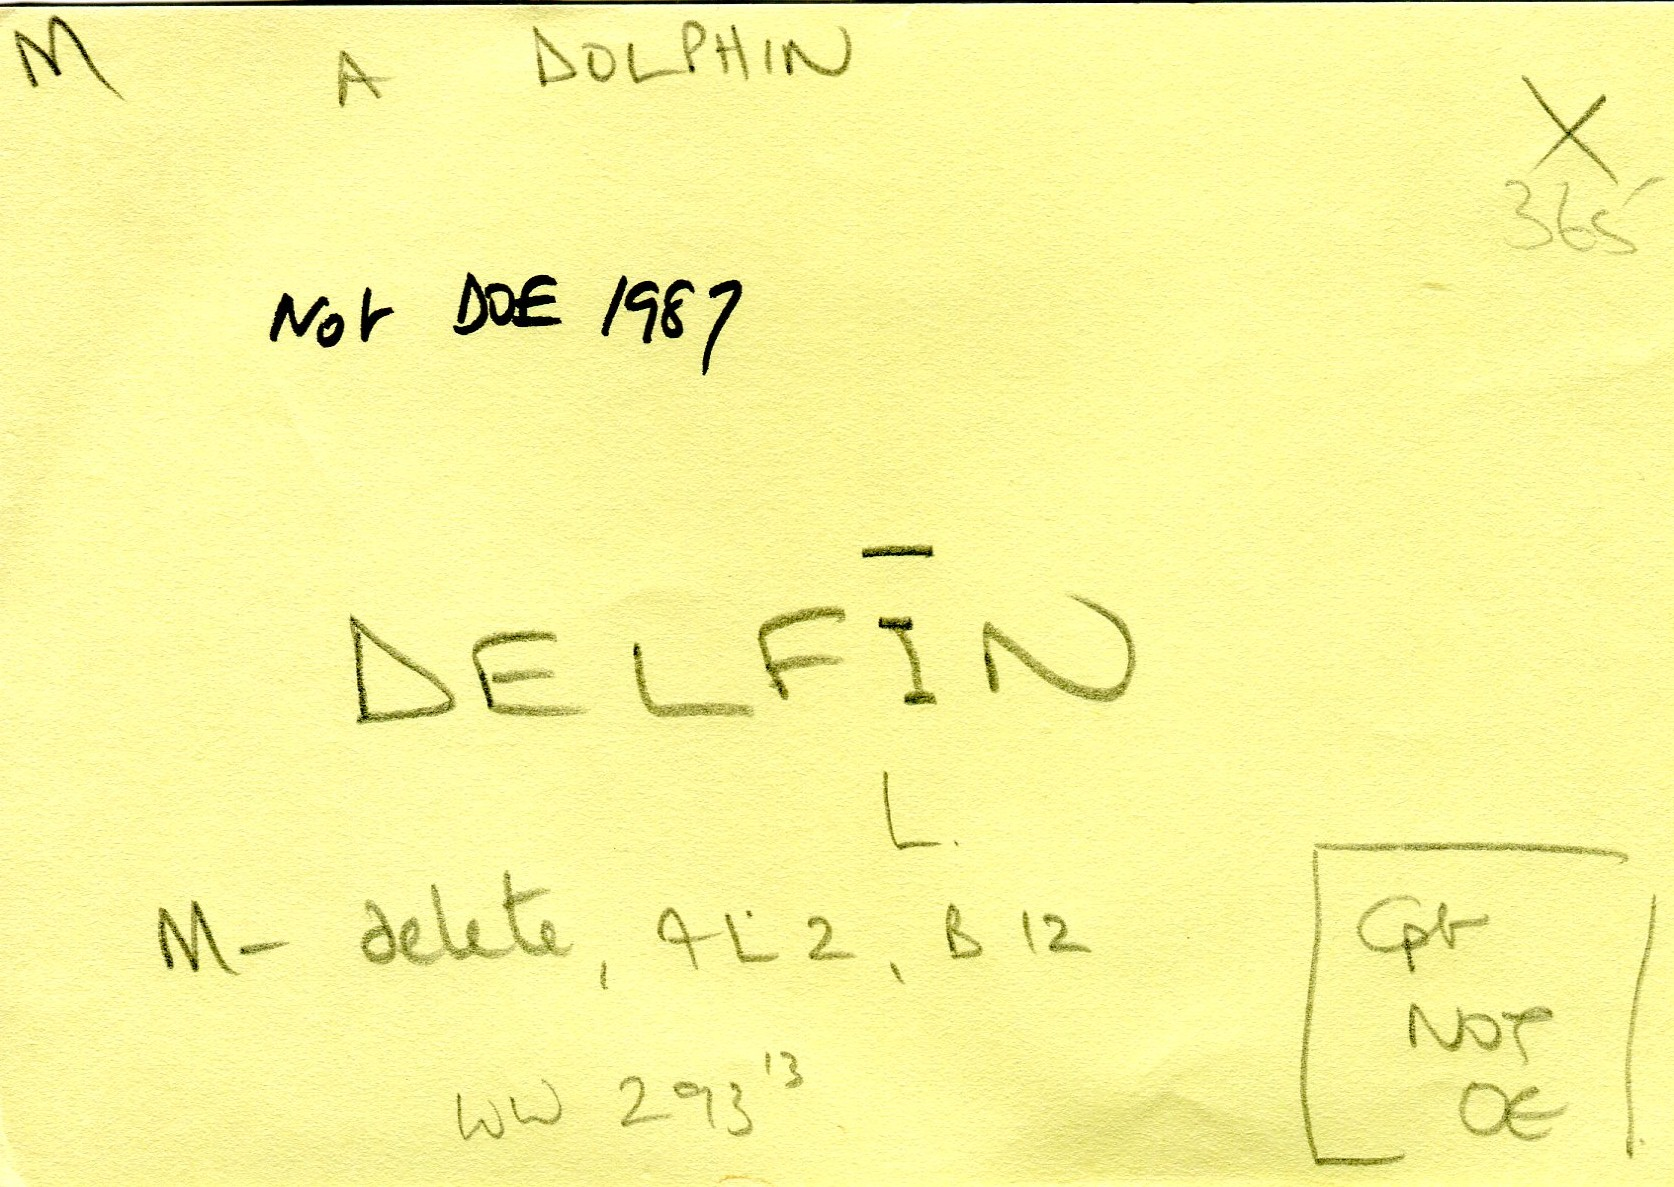
\includegraphics[width=\textwidth]{Stolk2021x/fig/Roberts-slip.jpg}
	\caption[]{\label{fig:Stolk2021x:Roberts-fig1} Yellow slip for \textit{delfin}.}
\end{minipage}
\begin{minipage}{.04\textwidth}\end{minipage}
\begin{minipage}{.48\textwidth}
  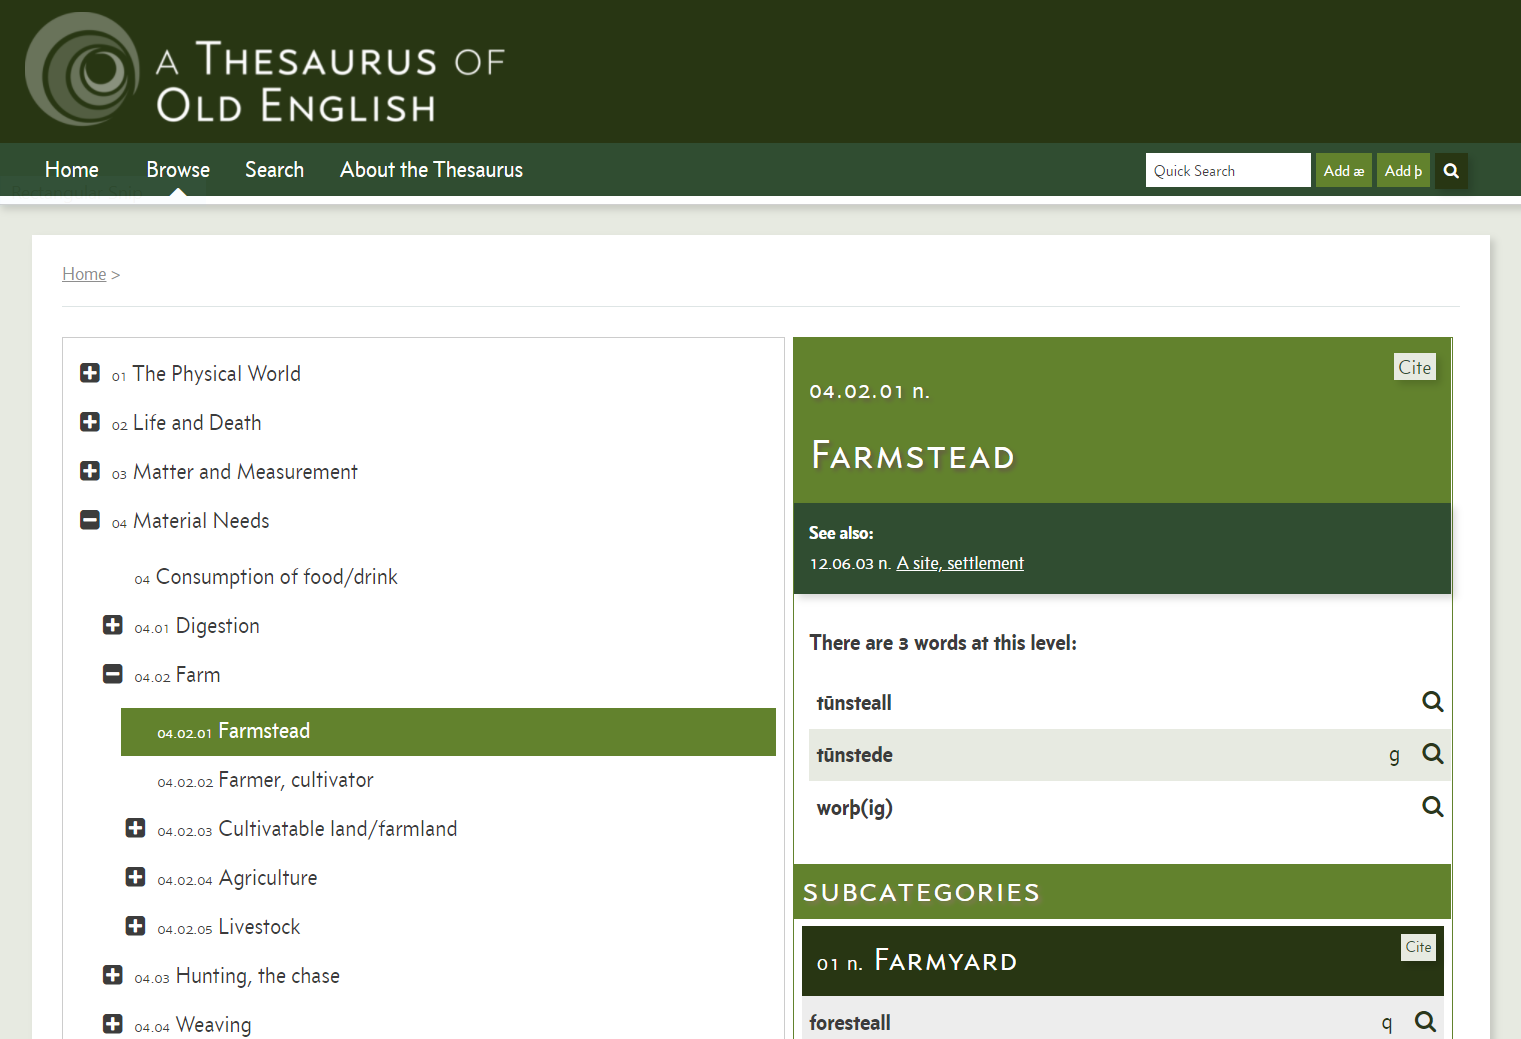
\includegraphics[width=\textwidth]{Stolk2021x/fig/Roberts-toe-online.png}
	\caption[]{\label{fig:Stolk2021x:Roberts-fig2} \textit{TOE} website hosted by the University of Glasgow.}
\end{minipage}
\end{figure}

Concluding her article, Roberts suggests a number of future ways in which scholars might interact with the \textit{TOE} data through the supplementation of additional information on individual words (e.g., dialects, origins, distribution across the corpus) and subsequent analysis of this information within the semantic hierarchy of \textit{TOE}. These research opportunities are facilitated by the web application Evoke, developed by Sander Stolk, whose contribution logically follows that of Roberts within the special issue.



\section{Evoke}

Approaching the \textit{TOE} from a digital humanities perspective, Sander Stolk describes how Evoke was created in response to various research needs, including user-friendly navigation, viewing, extension, linking, and analysis of thesaurus content (see Figure \ref{fig:Stolk2021x:Stolk-fig1} and \ref{fig:Stolk2021x:Stolk-fig2}) \cite{doi:10.1163/18756719-12340235}. Using Semantic Web technologies in order to make thesaurus content available in Linguistic Linked Data form, Evoke enables researchers to supplement existing thesauri, such as \textit{TOE}, without altering original datasets. 

\begin{figure}[htbp]
\centering
\begin{minipage}{.48\textwidth}
  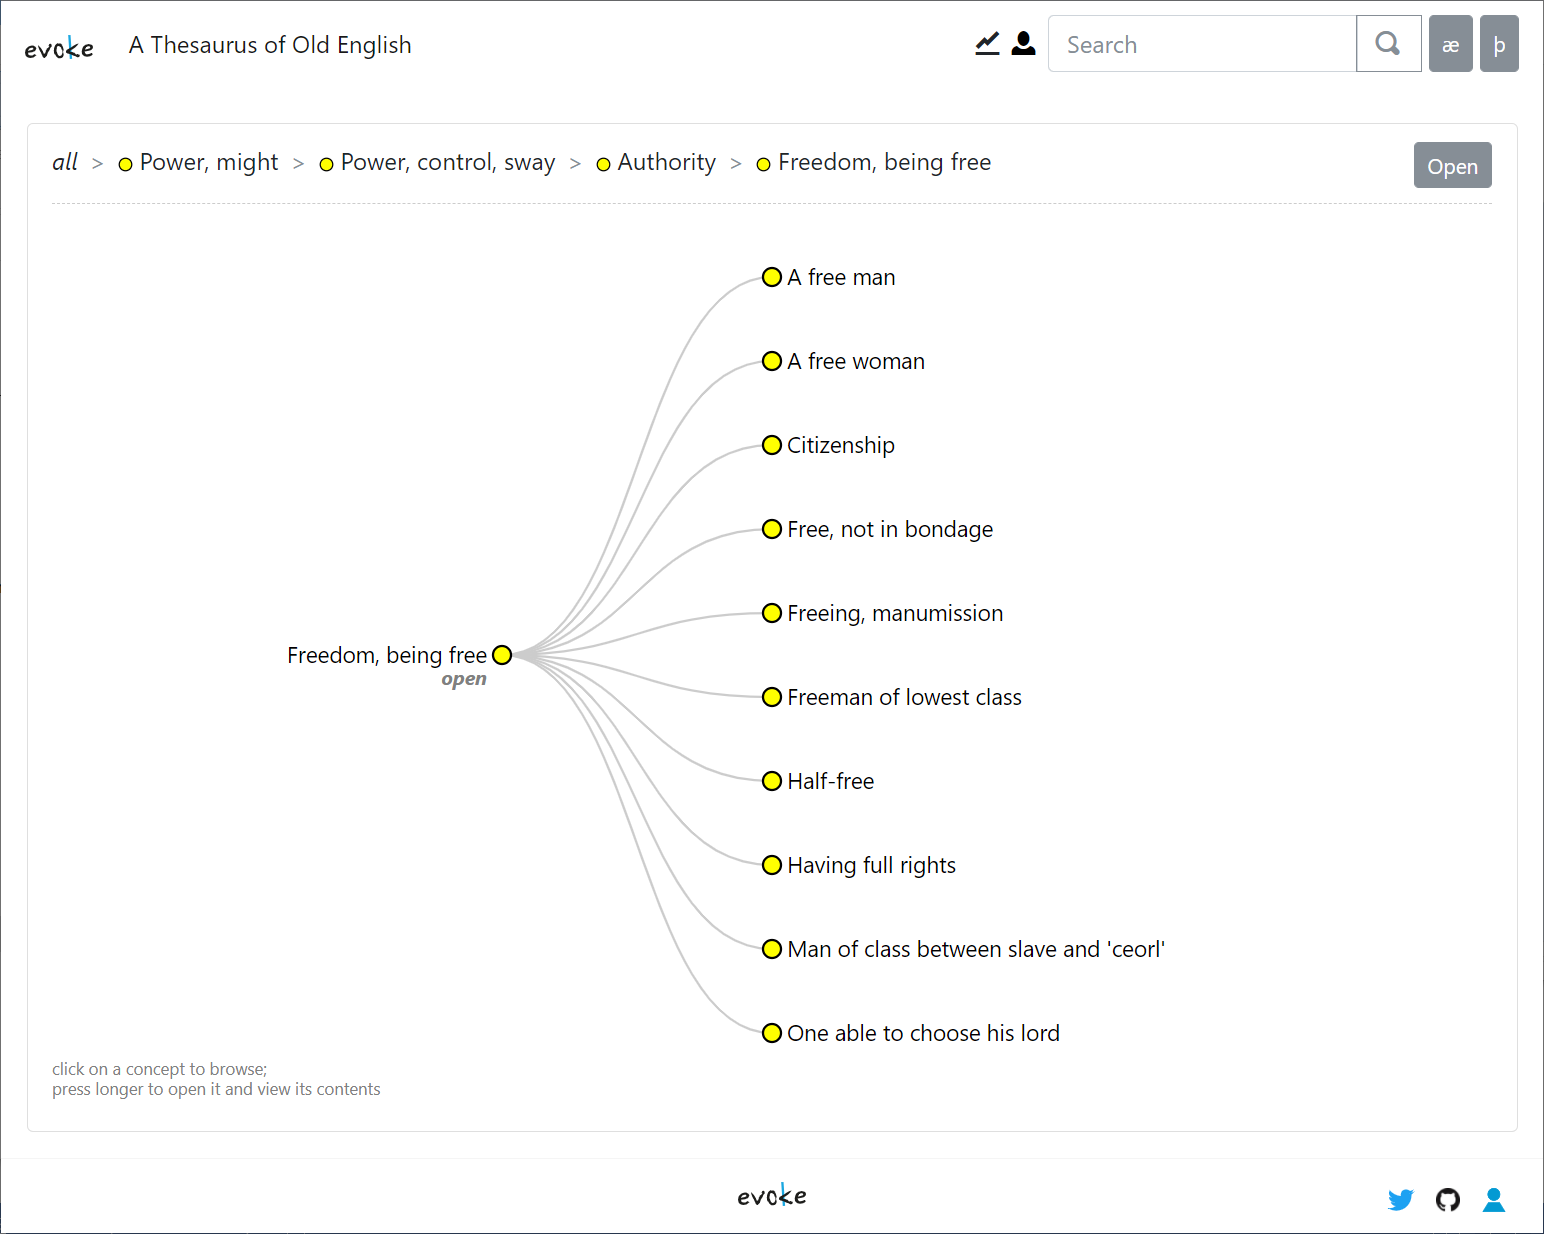
\includegraphics[width=\textwidth]{Stolk2021x/fig/Stolk-hierarchy.png}
	\caption[]{\label{fig:Stolk2021x:Stolk-fig1}Navigation of the \textit{TOE} semantic hierarchy in Evoke.}
\end{minipage}
\begin{minipage}{.04\textwidth}\end{minipage}
\begin{minipage}{.48\textwidth}
  \raggedleft
  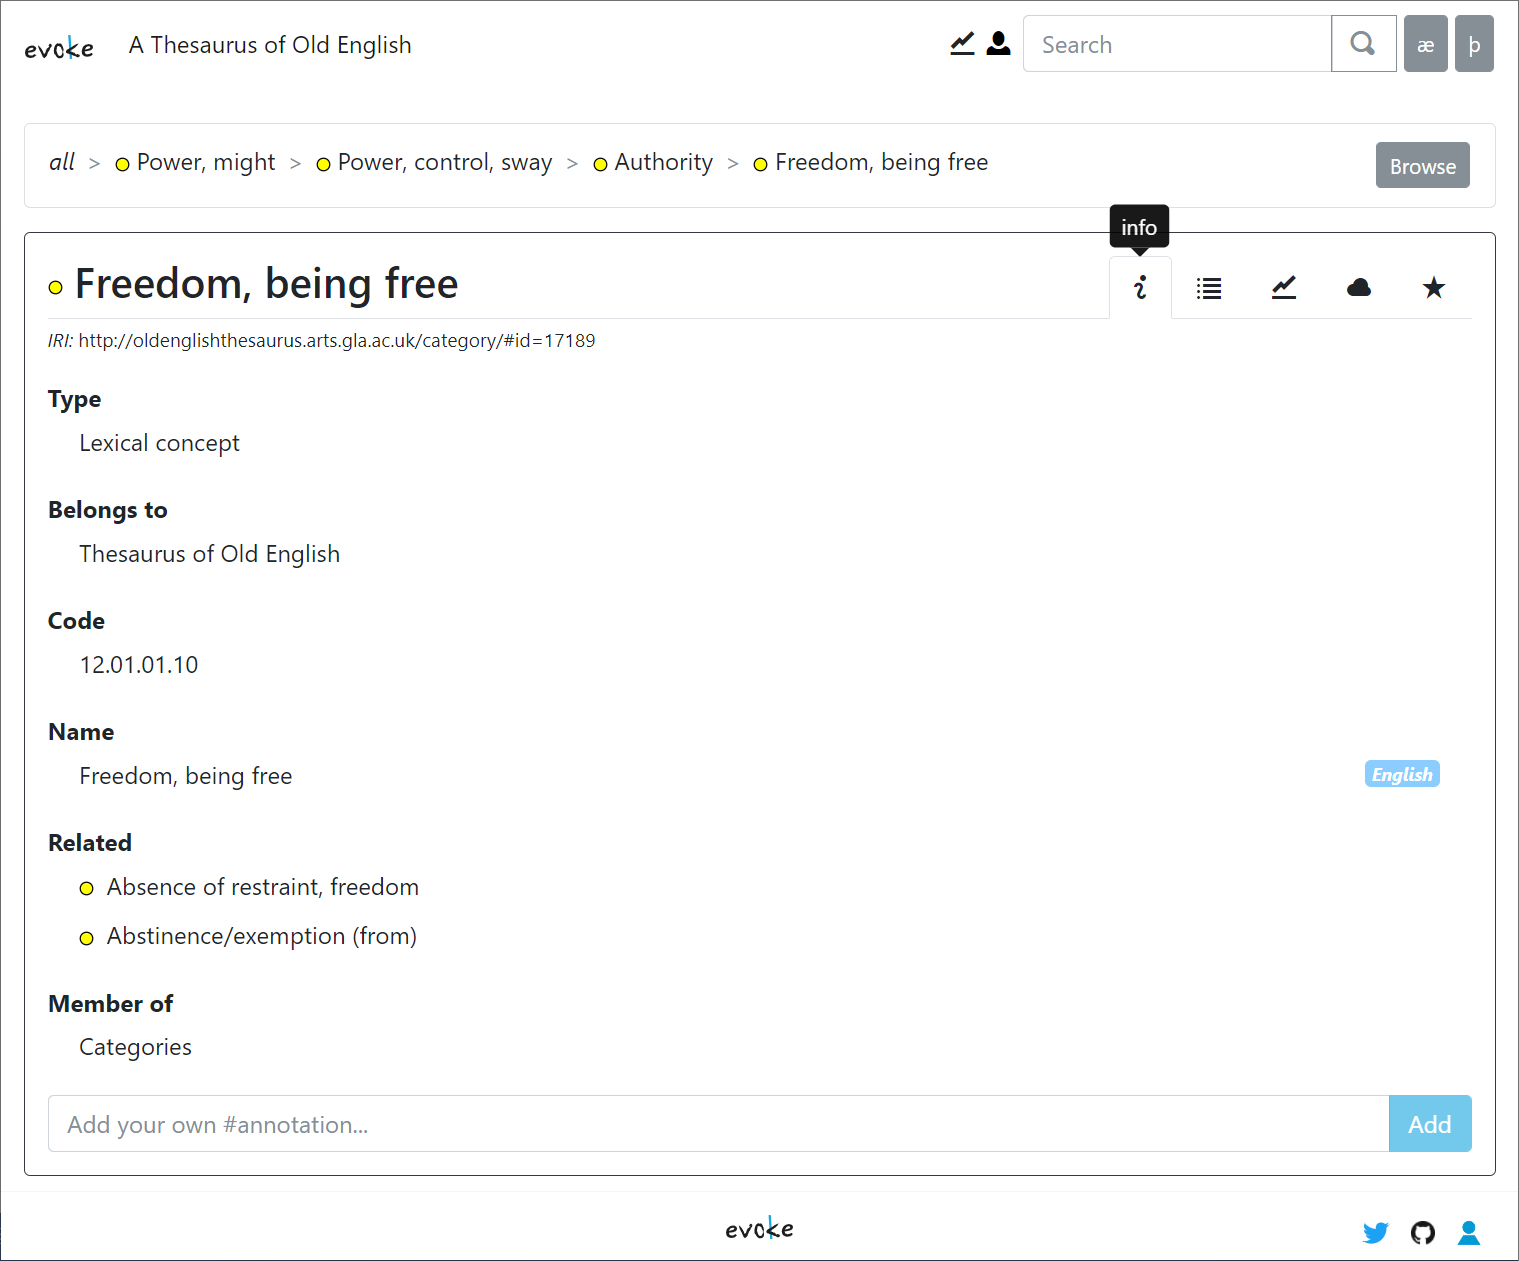
\includegraphics[width=\textwidth]{Stolk2021x/fig/Stolk-info.png}
	\caption[]{\label{fig:Stolk2021x:Stolk-fig2}Information on the \textit{TOE} category ``Freedom, being free'' in Evoke.}
\end{minipage}
\end{figure}

Stolk's contribution outlines how Evoke and a Linguistic Linked Data version of \textit{TOE} create new opportunities for research. All subsequent contributions to this special issue demonstrate the potential of Evoke to impact the study of Old English and, more broadly, the ways in which digital approaches, like Evoke, may affect the future of lexicography and onomasiology.\footnote{Note that the article in its entirety is included in this dissertation, preceding the current chapter.}
\end{comment}



\section{History of Old English lexicography}
\label{sect:Stolk2021x:cs-lexicog}

Several dictionaries of Old English have been published since the early modern period. The first was William Somner's \textit{Dictionarium Saxonico-Latino-Anglicum}, which appeared in 1659. Almost two centuries later, Joseph Bosworth published his \textit{A Dictionary of the Anglo-Saxon Language} in 1838. Fifty-six years later, John R. Clark Hall issued his \textit{A Concise Anglo-Saxon Dictionary for the Use of Students} in 1894. Both Bosworth's and Clark Hall's dictionary were further developed and expanded, which resulted in publications of supplements and revisions in the late nineteenth and the twentieth century.\footnote{In 1898, Thomas N. Toller published a revised edition of Bosworth's dictionary under the title `An Anglo-Saxon Dictionary'. A supplement became available in 1921 and an edition with ``enlarged addenda and corrigenda'', by the hand of Alistair Campbell, appeared in 1972. Clark Hall's dictionary exists in four editions, of which the last published in 1960.} 
%, followed closely by a revision of Bosworth's dictionary, published in 1898, developed by Thomas N. Toller. Work on both dictionaries continued: the second edition of Clark Hall's was published in 1916, a supplement to Bosworth-Toller became available in 1921, and an edition with ``enlarged addenda and corrigenda'' of Bosworth-Toller, by the hand of Alistair Campbell, appeared in 1972. 
\textit{TOE}, alongside University of Toronto's \textit{Dictionary of Old English}, is one of the more recent, major lexicographical works of Old English that is still being updated. %In her case study, Rachel Fletcher demonstrates that 
Developments in Old English lexicography can be scrutinised through the semantic domains available in \textit{TOE}, as demonstrated by the case study below.


\subsection{Charting lexicographic developments}

In her case study, Rachel Fletcher posited that Evoke and the Linguistic Linked Data version of \textit{TOE} enable investigations into the representation of the Old English lexicon throughout the history of Old English lexicography.\footnote{Rachel Fletcher presented the case study in a paper titled `Evoke and the History of Old English Lexicography: Preliminary Explorations' at the second EEMEE workshop (see Appendix \hyperref[Appendix8.B]{8.B}).} 
%As mentioned in section \ref{sect:Stolk2021x:toe},
As mentioned in the previous section, 
\textit{TOE} presents a filtered image of the early medieval English lexicon: it is based on the surviving texts, interpreted by scholars, and on prior dictionaries. Each lexicographic work reflects its aim, target audience, the knowledge of the lexis at that particular point in time, and the editorial choices inherent in lexicography. Utilizing Evoke, Fletcher's case study explored how the representation of the Old English lexicon in \textit{TOE} compares to its representation in earlier dictionaries, aiming to ``shed light not only on the subjectivity of the \textit{Thesaurus of Old English} (of which users should be aware) but on changing attitudes towards Old English and early mediaeval English culture over the history of scholarship''.\footnote{Citation taken from the paper abstract submitted to the workshop.}

%The Evoke platform allows users to interact with Thesaurus of Old English data in new ways, opening up possibilities for the study of Old English semantics. However, to make effective use of this tool, we need to be aware of the nature of the Thesaurus of Old English dataset. A Thesaurus of Old English is based on ‘the inherited wisdom of Anglo-Saxon scholarship’ and specifically on the Bosworth and Toller Anglo-Saxon Dictionary, Toller’s Supplement, Campbell’s Addenda, and the Clark Hall and Meritt Concise Anglo-Saxon Dictionary.  Therefore, it is appropriate to consider it in the context of the wider tradition of the lexicography of Old English, which reaches back to the sixteenth century. 


%In this paper, I will briefly describe how the Thesaurus of Old English and the Evoke platform fit into the tradition of Old English lexicography, before moving on to present some preliminary reflections on how data from older dictionaries could be integrated into Evoke. The results of a small proof of concept study, focused on a limited semantic field, will illustrate the potential applications of such an approach and how Evoke features might be used to scale up this kind of investigation.

The case study investigated five dictionaries alongside \textit{TOE}, including the two principal dictionaries on which \textit{TOE} is based. The five dictionaries are listed below in order of publication date. 
%
\begin{itemize}
\begin{comment}
\item 1659. \textit{Dictionarium Saxonico-Latino-Anglicum}. William Somner. Oxford: excudebat Guliel. Hall, pro authore.
\item 1772. \textit{Dictionarium Saxonico et Gothico-Latinum}. Edward Lye \& Owen Manning. London: excudebat Edm. Allen.
\item 1838. \textit{A Dictionary of the Anglo-Saxon Language}. Joseph Bosworth. London: Longman, Rees, Orme, Brown, Green \& Longman.
\item 1882-98. \textit{An Anglo-Saxon Dictionary}. Joseph Bosworth \& T. Northcote Toller. Oxford: Clarendon Press. (+ later supplements)
\item 1960. \textit{A Concise Anglo-Saxon Dictionary}, 4th edn. J. R. Clark Hall and H. D. Merritt. Cambridge: CUP.
\end{comment}

\item
W. Somner, \textit{Dictionarium Saxonico-Latino-Anglicum} (Oxford, 1659).
% excudebat Guliel. Hall, pro authore.

\item
E. Lye, \textit{Dictionarium Saxonico et Gothico-Latinum} (London, 1772).
% edidit (= published/circulated): Owen Manning
% excudebat Edm. Allen.

\item
J. Bosworth, \textit{A Dictionary of the Anglo-Saxon Language} (London, 1838).

\item
J. Bosworth and T. N. Toller, \textit{An Anglo-Saxon Dictionary Based on the Manuscript Collections of the Late Joseph Bosworth} (London, 1898), \textit{Supplement} by T. N. Toller (Oxford, 1921), with \textit{Enlarged Addenda and Corrigenda} by A. Campbell (Oxford, 1972).

\item
J. R. Clark Hall, \textit{A Concise Anglo-Saxon Dictionary}, 4th edn, with a supplement by H. D. Meritt (Cambridge, 1960).

\end{itemize}
%
Custom labels were created to identify each dictionary (`Som', `LM', `Bos', `BT', `HM') and used to mark \textit{TOE} word senses in Evoke to reveal which were recorded in the aforementioned dictionaries, thereby facilitating comparisons per semantic domain. 

In her case study, Fletcher focused on two \textit{TOE} categories: ``13.02.10.01.01 A warrior, fighter'' and ``14.01.04 A legal right''. Figure \ref{fig:Stolk2021x:Fletcher-fig1} shows an overview of Old English words denoting the former, including the established custom labels as assigned to each. A diachronic visualization of these findings is shown in Figure \ref{fig:Stolk2021x:Fletcher-fig2}. 
The results foreground that, compared to the current state of Old English lexicography, a disproportionate number of words denoting ``A warrior, fighter'' were not yet included in earlier dictionaries of Old English. Notably absent in these dictionaries are so-called kennings and other compounds found in poetic diction (e.g., \textit{scildwiga} [lit. ``shield warrior''] and \textit{heoruwulf} [lit. ``sword wolf'']). Fletcher posited that these findings reflect the historical interest in Old English lexicography, which focused initially on legal and historical sources (e.g., laws, chronicles) and expanded later to poetic texts.\footnote{Fletcher indicated there are various reasons why the poetic lexicon received less attention in early scholarship, including the inaccessibility of some poetic texts (e.g., Vercelli MS was only rediscovered in the nineteenth century) and a higher difficulty in interpreting them (due to their freedom in syntax, lack of Latin parallel texts, and, importantly, use of hapax legomena, words that occur in only a single text throughout the corpus).} %Although word variety found in poetry was not reflected in early dictionaries, knowledge on the meaning of these words may not have been lacking, since the various components of these kennings were often included as separate entries. 
In the future, Fletcher concluded, further developments in Old English lexicography may change this picture. Ongoing work on Toronto's \textit{Dictionary of Old English}, is improving scholarly understanding, and surfacing of new material will influence how researchers perceive and study Old English language and culture. %Lexicography on Old English remains a work in progress.

\begin{figure}[h]
\centering
\begin{minipage}{.48\textwidth}
  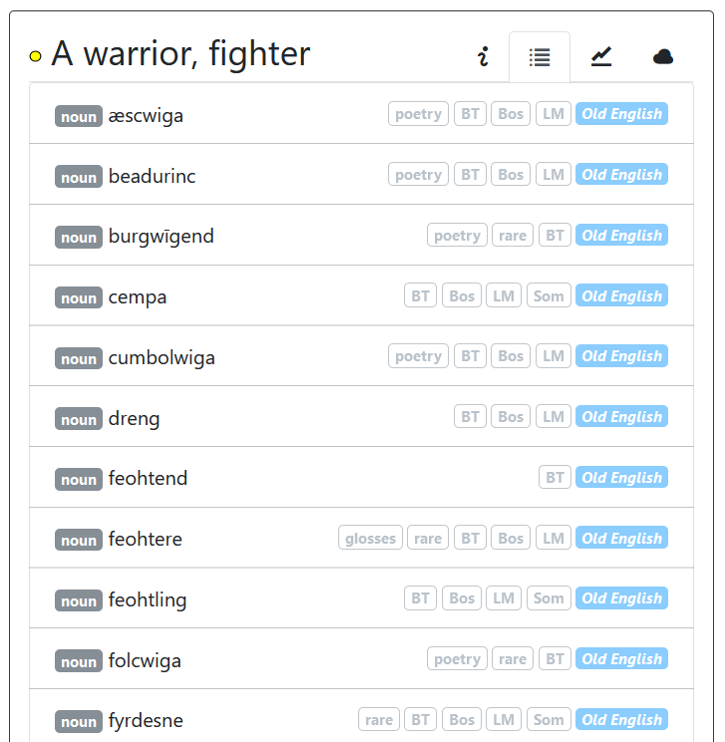
\includegraphics[width=\textwidth]{Stolk2021x/fig/Fletcher-warrior.png}
	\caption[]{\label{fig:Stolk2021x:Fletcher-fig1}List in Evoke of Old English words denoting ``A warrior, fighter'', annotated with custom labels indicating dictionaries in which each word has been recorded.}
\end{minipage}
\begin{minipage}{.04\textwidth}\end{minipage}
\begin{minipage}{.48\textwidth}
  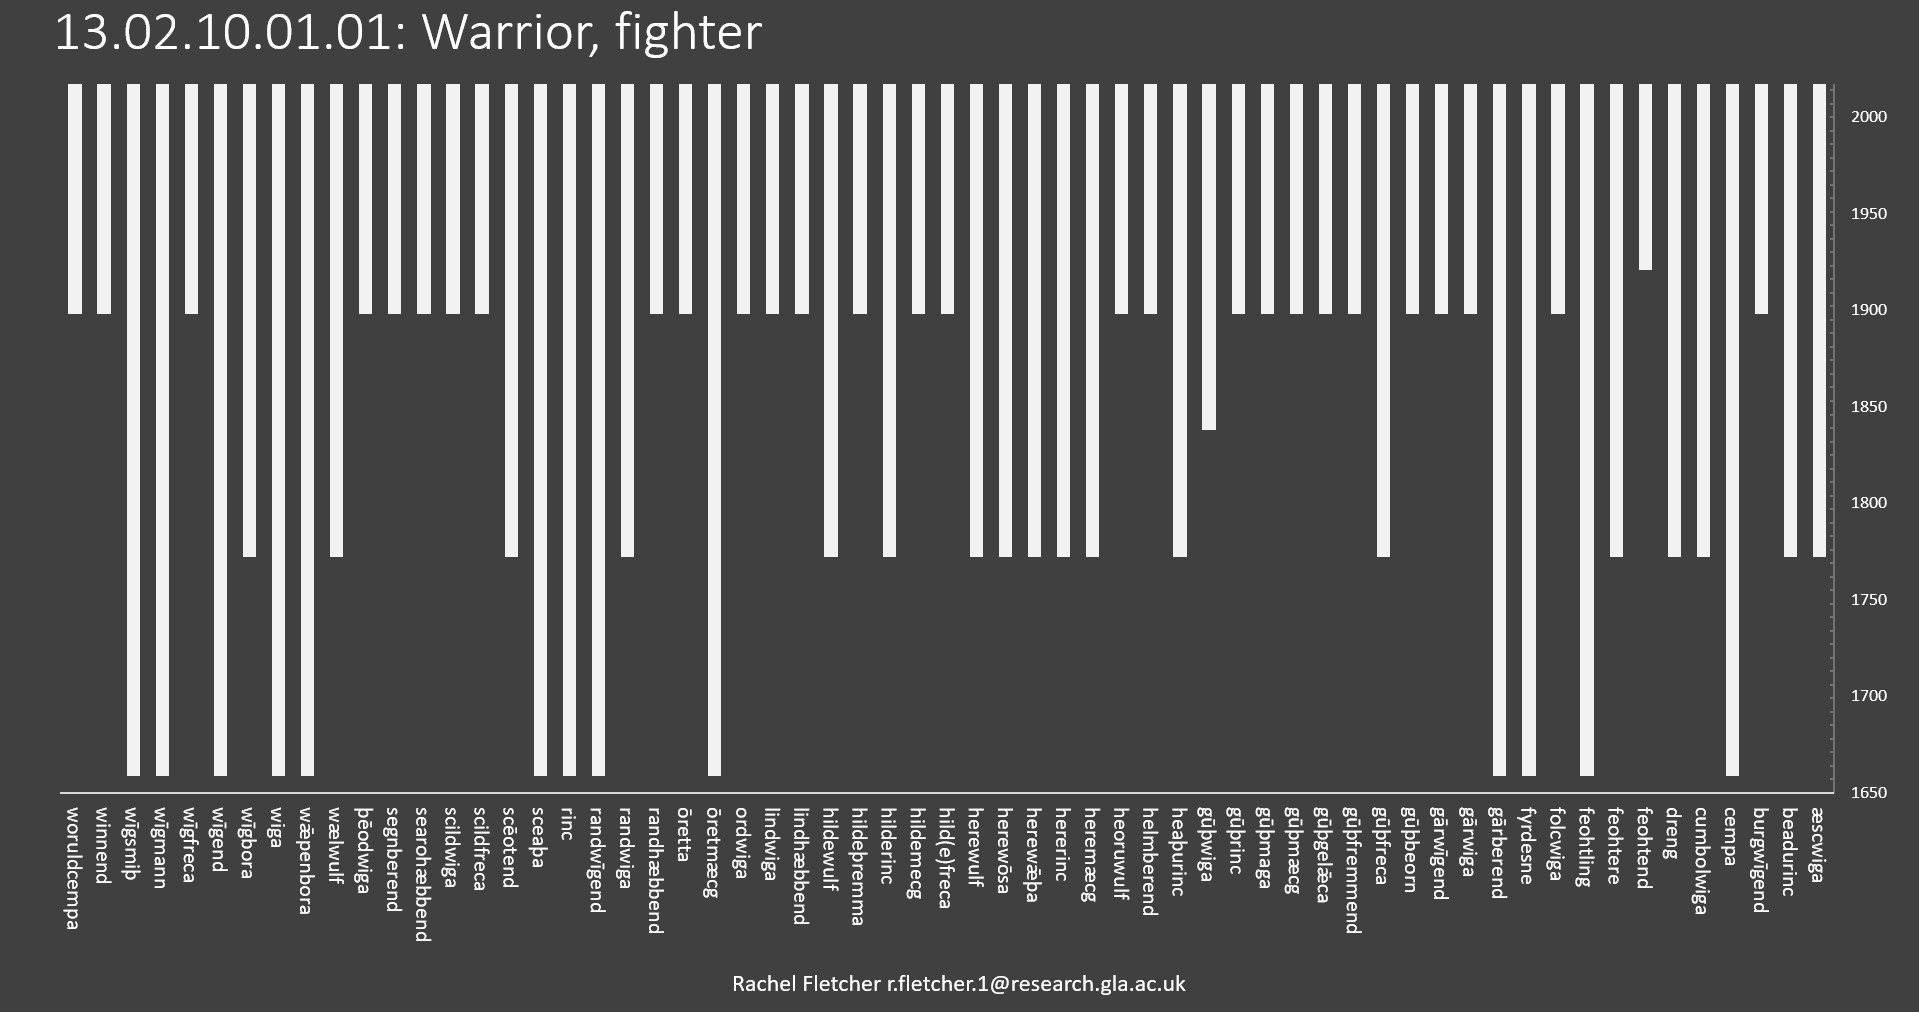
\includegraphics[width=\textwidth]{Stolk2021x/fig/Fletcher-warrior-barcode.png}
	\caption[]{\label{fig:Stolk2021x:Fletcher-fig2}Bar chart of Old English words denoting ``A warrior, fighter'' and the dates from which they were first recorded in an Old English dictionary.}
\end{minipage}
\end{figure}

Fletcher's work foregrounds the value of custom labels for exploring aspects besides stylistics or diachronic developments of a language. 
Her case study illustrates the use of thesauri for the study of lexicographic practices, although such explorations are not without challenges. Variation in spelling amongst the dictionaries, differences in the granularity of sense definitions, and reinterpretation of words as belonging to another semantic domain %entirely 
can hamper straightforward application of labels and alter what can be deduced from subsequent analysis. Even so, Fletcher's case study demonstrated that \textit{TOE} can provide a semantic framework under which concepts and entire domains can be scrutinized in terms of their lexicographic developments. Annotation functionality in Evoke enables viewing and sharing such findings. The chart in Figure \ref{fig:Stolk2021x:Fletcher-fig2} indicates a need for further visualizations beyond those currently available in Evoke, and potentially including temporal information, that may inform future development of the web application. %Similar to lexicography on Old English, advances in functionality offered for research remain welcome.

\begin{comment}
\textcolor{red}{
\subsection{Sandor Chardonnens - what would we know without the discovery of a given text / how did it impact our understanding of OE?}
\begin{itemize}
\item 	i.e., filter all words marked Beowulf and flagged ``o''
\item 	what remains ought to be everything not just found in Beowulf but also elsewhere
\end{itemize}
}
\end{comment}




\section{Stylistics of Old English writing}
\label{sect:Stolk2021x:cs-stylistics}

Historical language thesauri can also be valuable resources for exploring stylistics of specific texts, authors from the historical period, or entire genres. Two EEMEE case studies demonstrated this avenue of research for the Old English context through enrichment of the \textit{TOE} dataset with custom labels. Their subsequent analyses in Evoke have led to new insights into the language use in specific texts (\textit{Beowulf}, \textit{Andreas}, the \textit{Old English Martyrology}) or by a specific author (Ælfric of Eynsham). These case studies are discussed in separate subsections below.

%The stylistics of Old English texts, certain authors of the period, or entire genres can thus be examined. Two case studies within EEMEE explore this avenue of research, each of which discussed in a separate subsection below.

\subsection{Onomasiological profiles of Old English texts}

%Enriching the \textit{TOE} dataset with custom labels, through Evoke, can lead to new insights into the language use by specific authors or in specific contexts. 
In his case study, Thijs Porck demonstrated how Evoke can be used to investigate the lexis used in individual Old English texts.\footnote{Porck, `Onomasiological Profiles of Old English Texts'.} %\cite{doi:10.1163/18756719-12340236}
By tagging all words that occur in \textit{Beowulf}, \textit{Andreas}, and the \textit{Old English Martyrology}, Porck expanded the Linguistic Linked Data version of \textit{TOE} with information that allows users to navigate the vocabulary in these specific texts through the semantic hierarchy of the thesaurus. In effect, this process has created three workable prototypes of thesauri, specific to the selected texts, which have been made publicly available in Evoke for anyone to browse and analyse (see Appendix \hyperref[Appendix8.A]{8.A}).

By combining the \textit{TOE} dataset in Evoke with additional information on individual texts, Porck was able to navigate and analyse the vocabulary use in these medieval texts. Figure \ref{fig:Stolk2021x:Porck-fig1}, for example, lists Old English words denoting ``A man, warrior'' and the labels assigned to them. Overviews such as these allow differences in word use between Old English texts to be discerned. The word \textit{ceorl}, for instance, was shown to occur in the poem \textit{Beowulf} but not in \textit{Andreas} or the \textit{Old English Martyrology}, whereas \textit{þegn} occurs in all three texts. 

\begin{figure}[htbp]
\centering
\begin{minipage}{.48\textwidth}
  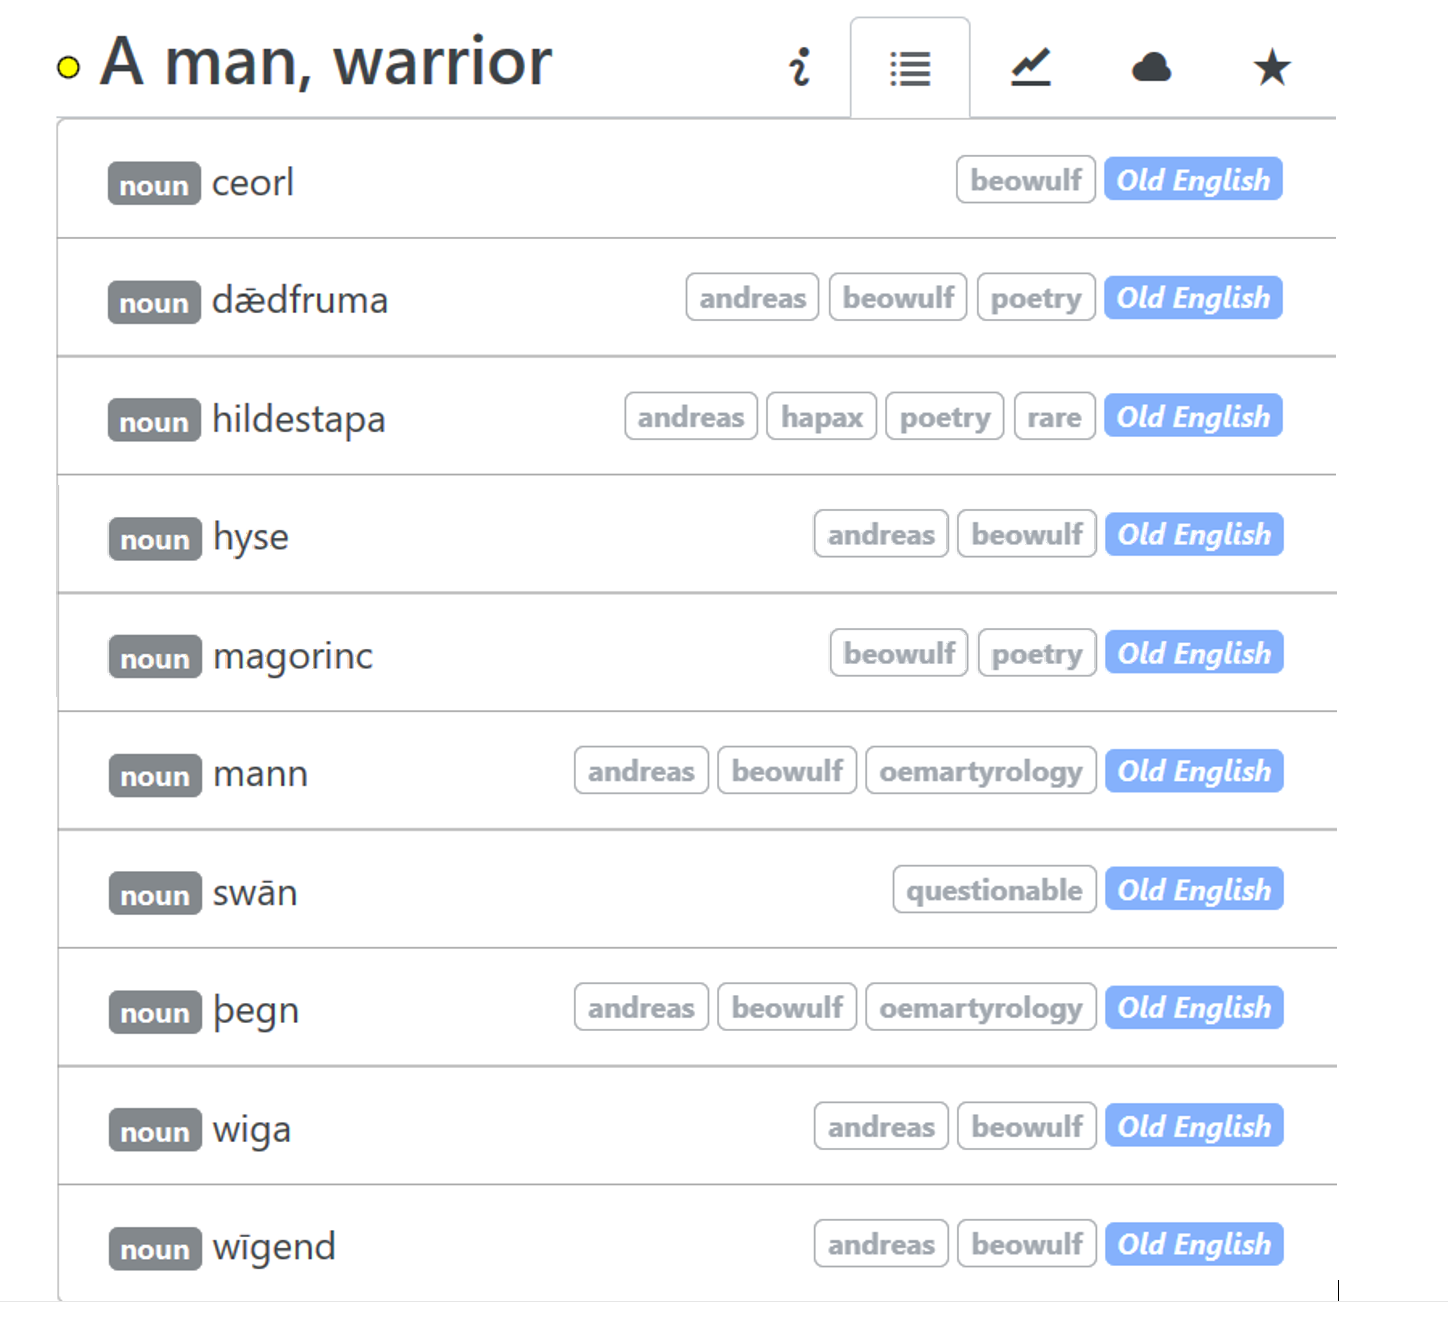
\includegraphics[width=\textwidth]{Stolk2021x/fig/Porck-warrior.png}
	\caption[]{\label{fig:Stolk2021x:Porck-fig1}List in Evoke of Old English words (and their labels) denoting ``A man, warrior''.}
\end{minipage}
\begin{minipage}{.04\textwidth}\end{minipage}
\begin{minipage}{.48\textwidth}
  \raggedleft
  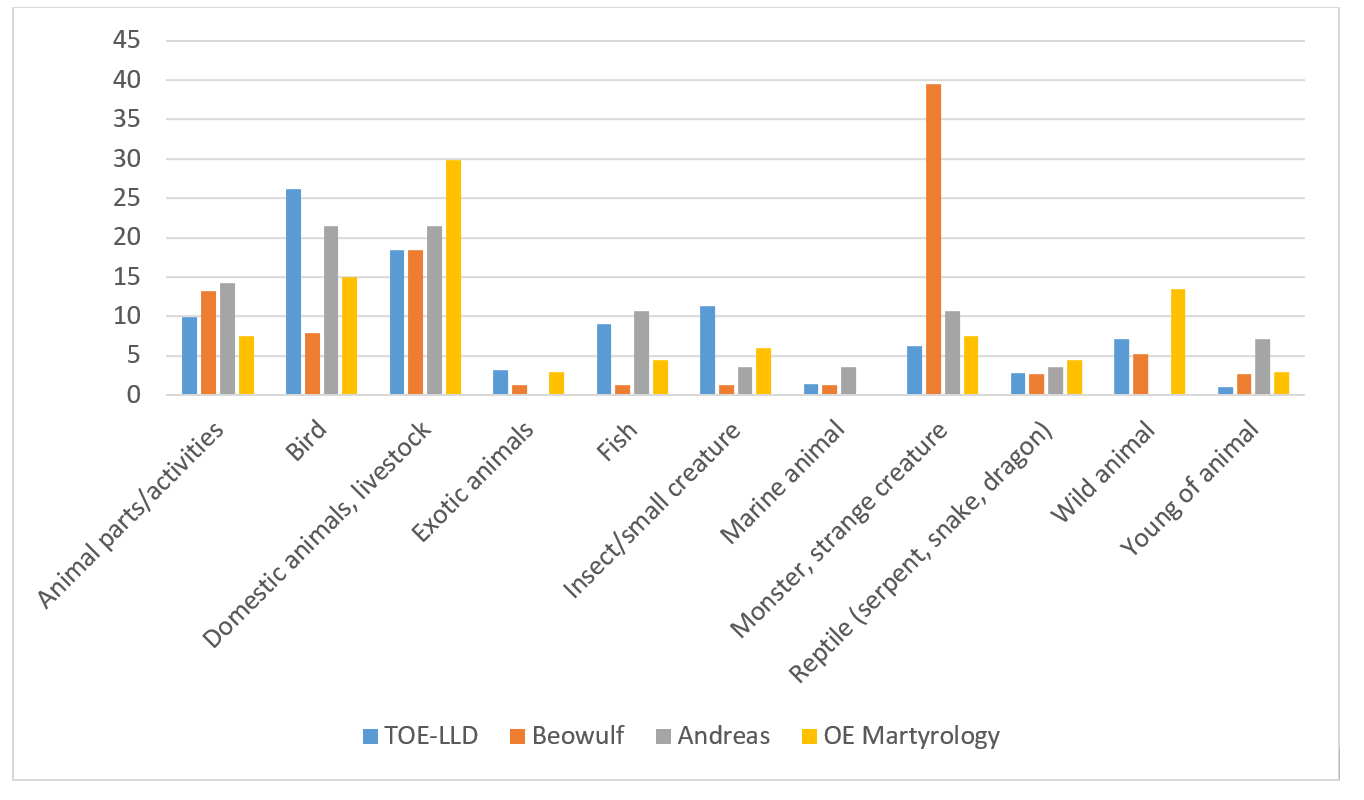
\includegraphics[width=\textwidth]{Stolk2021x/fig/Porck-animals.png}
	\caption[]{\label{fig:Stolk2021x:Porck-fig2}Onomasiological profiles of various Old English texts for the semantic field of ``Animal''.}
\end{minipage}
\end{figure}

Additionally, the combined information in this case study can be used to create semantic fingerprints, or `onomasiological profiles', of individual Old English texts through the statistics provided by the interface of Evoke. In contrasting such profiles for individual Old English texts, Porck showed how new and distinctive patterns of vocabulary use can be brought to light. To illustrate, Figure \ref{fig:Stolk2021x:Porck-fig2} captures vocabulary use in the semantic field of ``Animal'' across the entire corpus of Old English and within the three different Old English texts, specifically. Each text, Porck argues, ``shows distinctive patterns of vocabulary use that can be related to the roles that animals play in the individual texts''.\footnote{Ibid., p. 378.} For instance, most of the words used in the \textit{Old English Martyrology} within this semantic field are found in the categories of ``Domestic animals, livestock'', ``Bird'' and ``Wild animal'', which matches scholarly observations on medieval hagiography. As Porck explains, ``typically, saints are served by domestic animals and birds, while wild animals either miraculously come to their aid or represent devils in disguise''.\footnote{Ibid., p. 379.} \textit{Beowulf} displays a vastly different picture. By far, the category of ``Monster, strange creature'' contains the majority of the words used within this field, which is unsurprising given the prominent role of monsters within the poem.

On a higher, more abstract level, Porck employed onomasiological profiles of the three Old English texts to obtain insights into aspects that include their poetic characterization and degree of ambiguity. On the first aspect, Porck remarks that the ``lexicon of \textit{Beowulf} consists of more entries exclusively found in poetic contexts (30.66\%) than that of \textit{Andreas} (20.60\%), while the lexicon of the prose \textit{Old English Martyrology} is, naturally, devoid of poetic vocabulary''.\footnote{Ibid., p. 370.} On the degree of ambiguity found in the texts, which is based on the number of polysemous senses attributed to each lexical entry, he notes that texts marked with a higher level of words found solely in poetic contexts (i.e., \textit{Beowulf} and \textit{Andreas}) are more likely to be low in polysemous senses than other texts (i.e., the \textit{Old English Martyrology}) and yield a lower degree of ambiguity.\footnote{Ibid., pp. 371-2.}

Porck's use of Evoke and \textit{TOE} exemplifies the value of linking resources and how combining sets of information allows researchers to obtain a picture hitherto unavailable. In fact, an onomasiological analysis of these Old English texts would not go amiss in the introductions to their respective scholarly editions. A case in point is the fourth edition of \textit{Klaeber's Beowulf}, which contains information on, amongst others, the diction, orthographic characteristics, and narrative structure. This material positions the poem in its literary and linguistic context --- a positioning which would benefit from insights into the semantic domains present in this text. Contrasts with contemporary texts, across genres, and diachronic developments could, over time, be added to such sections on onomasiological characteristics. Indeed, much remains to be explored. Only a few selected fields have been scrutinized, thus far, using the analysis functionality of Evoke. The textual thesauri fashioned by Porck, publicly available in Evoke, will undoubtedly lead to a deeper understanding of these and other texts in the future.



\subsection{Exploring `Ælfrician' vocabulary}

Amos van Baalen used Evoke in a manner similar to that of Porck.\footnote{Van Baalen, `Identifying, Categorising and Exploring ``Ælfrician'' Vocabulary using the \textit{Dictionary of Old English}, \textit{A Thesaurus of Old English} and Evoke'.} %\cite{doi:10.1163/18756719-12340237}
However, rather than creating onomasiological profiles of texts, van Baalen fashioned one for an individual author: Ælfric of Eynsham (c.955x957–c.1010). This abbot was one of the most prominent and prolific writers of the period. His vocabulary -- and its influence on the surviving Old English lexis -- is therefore important for our understanding of the language and culture of early medieval England. In researching Ælfric's vocabulary, van Baalen employed the \textit{Dictionary of Old English} and prior scholarship to identify and categorize the lexis that is characteristic for the works of Ælfric. The results were used to establish an onomasiological profile in Evoke of the abbot's characteristic vocabulary.

Rather than tagging all words known to have been used by Ælfric, van Baalen first established and categorized those words that had been identified as being representative of `Ælfrician' vocabulary. Words that are predominantly used by Ælfric (such as \textit{cāsus} `case' and \textit{forþearle} `very much, greatly') were marked in Evoke and subsequently analysed in order to create an onomasiological profile, which allowed van Baalen to comment on such aspects as the ambiguity, synonymy, specificity, and semantic distribution of the words characteristic of Ælfric's writing (see Figure \ref{fig:Stolk2021x:VanBaalen-fig1} and \ref{fig:Stolk2021x:VanBaalen-fig2}).\footnote{A list of all words found to be typical of Ælfric's writings, listed under the various categories established in this case study, is included as an appendix to the article by van Baalen.} The use of custom labels in Evoke ensured that the various categories established by van Baalen could be represented that convey the frequency of a word's use by Ælfric, as recorded in \textit{DOEC}, compared to its frequency in surviving Old English texts by other authors.

\begin{figure}[htbp]
\centering
\begin{minipage}{.48\textwidth}
  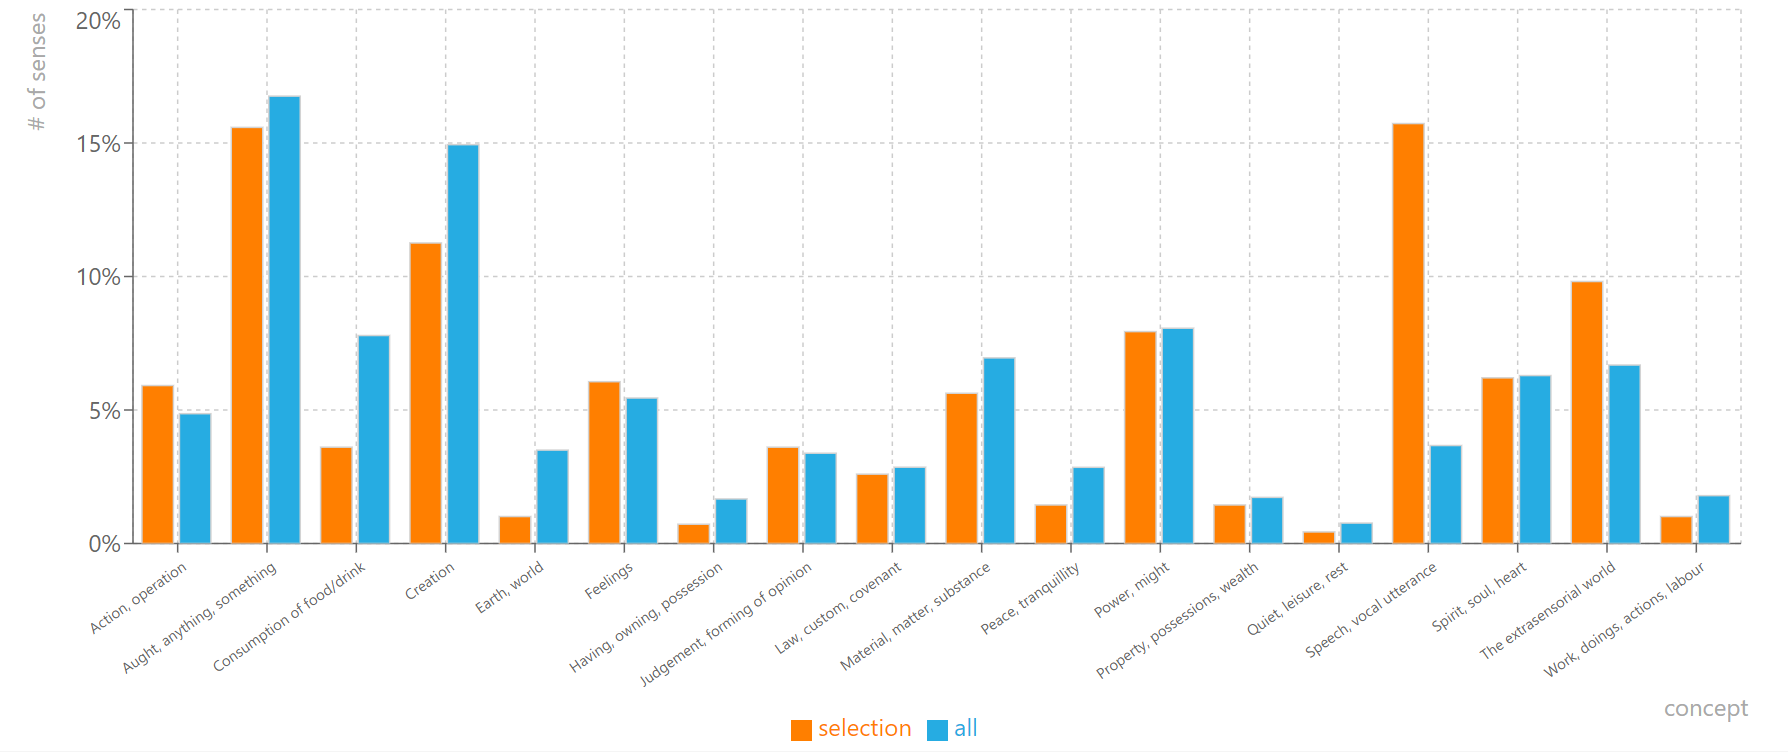
\includegraphics[width=\textwidth]{Stolk2021x/fig/VanBaalen-categories.png}
	\caption[]{\label{fig:Stolk2021x:VanBaalen-fig1}Semantic distribution of Ælfrician vocabulary contrasted with that of all Old English lexis.}
\end{minipage}
\begin{minipage}{.04\textwidth}\end{minipage}
\begin{minipage}{.48\textwidth}
  \raggedleft
  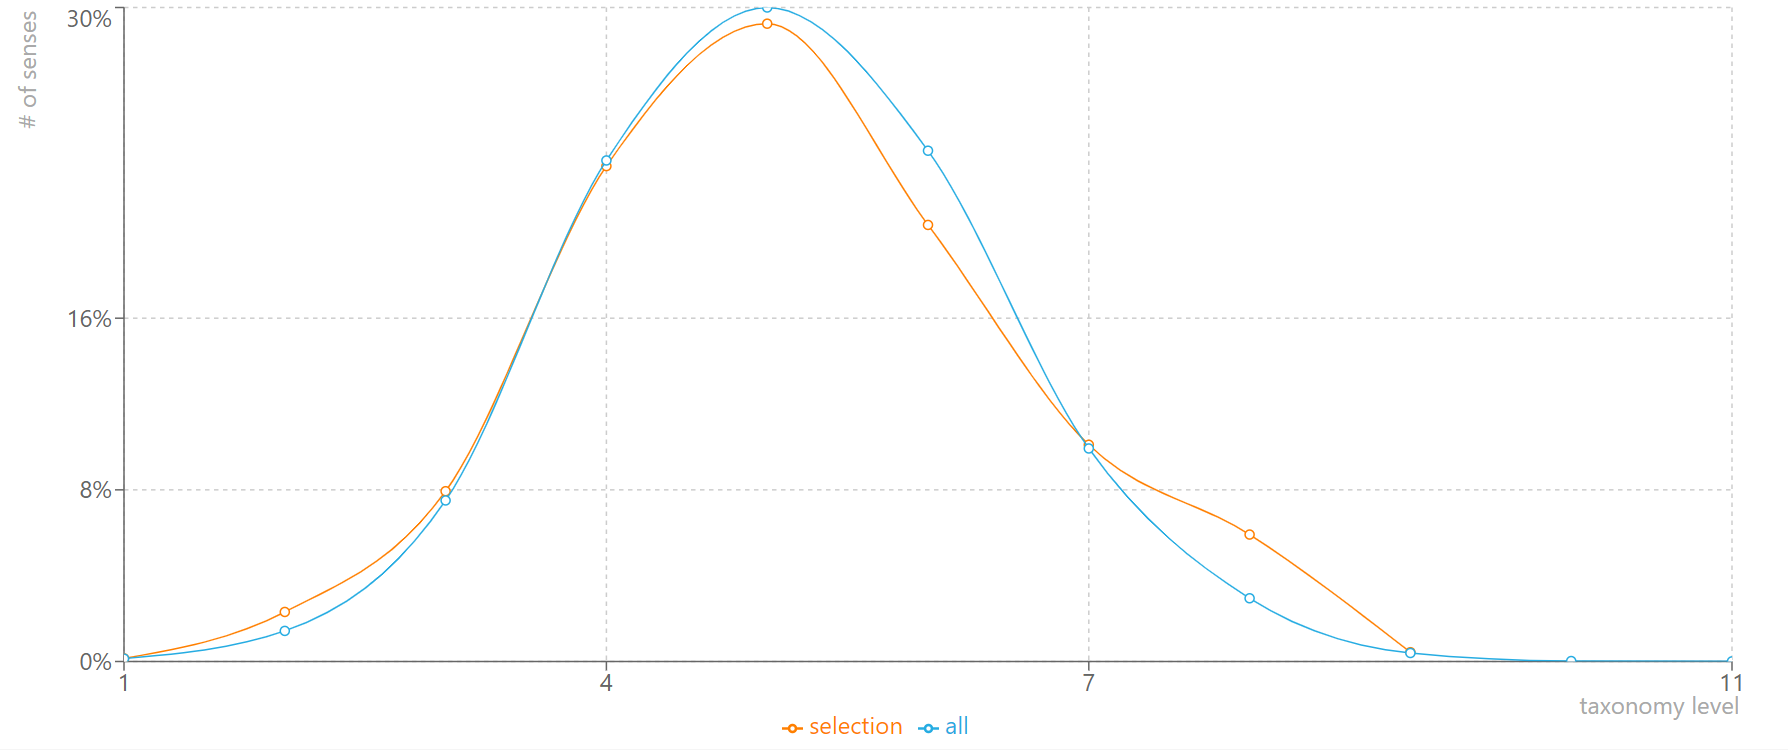
\includegraphics[width=\textwidth]{Stolk2021x/fig/VanBaalen-specificity.png}
	\caption[]{\label{fig:Stolk2021x:VanBaalen-fig2}Specificity of Ælfrician vocabulary contrasted with that of all Old English lexis.}
\end{minipage}
\end{figure}

Van Baalen's work with Evoke establishes a working method to quantify and pinpoint distinctive authorial preferences within semantic domains. His approach demonstrates that the annotation system of Evoke is an effective means for scholars to add information to a thesaurus and to view as well as query the results. An exciting aspect of this case study is that the categorizations for Ælfrician vocabulary, added by the scholar as labels to the lexis recorded in \textit{TOE}, hint towards future directions in which thesauri and corpora are more closely integrated. Once word attestations are linked to their corresponding entries in thesauri, onomasiological profiles can consider matters of frequency and predominant usage.\footnote{Standardizing the modelling of frequency and attestations in Linguistic Linked Data is currently being pursued (Chiarcos et al., `Modelling Frequency and Attestations for OntoLex-Lemon').} %\cite{chiarcos-etal-2020-modelling}.
Moreover, such an integration would, effectively, allow onomasiological profiles to be generated for authorial preferences, specific texts, and even entire genres.


\begin{comment}
\textcolor{red}{
\section{Semantic field and connotations and pragmatics}
\subsection{Porck - A thesaurus of the human life cycle}
\begin{itemize}
\item 	Tagging `old age'  (i.e., relevant words… or potentially relevant)
\item 	Tagging `[has been applied to] human'  (i.e., as opposed to animals)
\item 	Tagging `decrepitude', `grief', `authority', `wisdom', etc.   (i.e., connotations)
\item 	Marking ghost words
\item 	Marking words not related to old age, but falsely categorized as such
\end{itemize}
}
\end{comment}


\section{Diachronic developments of Old English}
\label{sect:Stolk2021x:cs-diachronic}

%Since \textit{TOE} records the earliest variant of English, the lexicographic work 
%\textit{TOE} may be employed to research language change in the earliest variant of English. Even so, the thesaurus content by itself lacks temporal distinctions necessary to draw any conclusions on the matter. As Richard Dance points out, 
In its current, traditional form, \textit{TOE} does not allow researchers to study changes across the Old English period, since, as Richard Dance points out, the thesaurus treats its items as ``a single geographically and temporally indistinguishable mass'', ignoring diachronic differences between, e.g., Early West Saxon and Late West Saxon.\footnote{Dance, Review of \textit{TOE1} (p. 313).} However, Evoke's functionality to add custom labels to words does allow for diachronic investigations by incorporating such distinctions. %The Linguistic Linked Data form of \textit{TOE} facilitates expanding the thesaurus to incorporate such distinctions in the Old English lexis. 
Information on the origins of words can be added, too, in a similar manner. Jane Roberts 
%, in her reflection on the creation of \textit{TOE},
asserts that such practice, e.g., flagging Latin loan words or those with an Old Norse origin, ``could lead to the examination of loan translation and word formation, dialect vocabulary, etc.; and Evoke provides a welcome platform for such undertakings''.\footnote{Roberts, `\textit{A Thesaurus of Old English}: The Pilot Study for the Glasgow Historical Thesaurus', p. 312.} The following subsection discusses one approach towards diachronic investigations, undertaken by Khan et al., who have mapped conceptual variation in \textit{TOE} through the web application Evoke.

\begin{comment}    
\textcolor{red}{
\subsection{Etymology and dating of words and word senses}
\begin{itemize}
\item (e.g., Roberts: indicate origins as Latin, Old Norse, etc.)
\item (e.g., Amos: 10th , 11th and 12th century texts)
\item (e.g., Sandor: relative dating, trace development of word and meaning)
\end{itemize}
FROM CHAPTER 1.
Explicit diachronic information that further subdivides the period treated, however, is not available in every historical language thesaurus. \textit{TOE}, in fact, treats its items as “a single geographically and temporally indistinguishable mass”, ignoring diachronic differences between, e.g., Early West Saxon and Late West Saxon.\footnote{Dance, Review of \textit{TOE1} (p. 313).}
adding distinctions would make for an interesting project
}
\end{comment}


\subsection{Mapping conceptual variation and diachronic changes}

%Turning to the field of Emotion studies, 
The case study by Khan et al. explored how Evoke may be used to visualize, navigate, and investigate conceptual mappings within the Old English vocabulary of \textsc{shame}.\footnote{Khan et al., `Mapping Conceptual Variation through \textit{A Thesaurus of Old English} and Evoke'.} %\cite{doi:10.1163/18756719-12340238} 
The authors, after having established a list of 28 words and expressions for \textsc{shame} based on \textit{TOE} and other lexicographic resources, charted conceptual variation in this vocabulary through two classifications. Firstly, each word or expression was classified as a metaphorical mapping. For instance, the verb \textit{ārēodian} (``to blush, be ashamed'', lit. ``to turn red'') belongs to the mapping \textsc{emotion is redness in the face}. Secondly, the development of each word or expression for \textsc{shame} was classified into one of four diachronic scenarios based on whether or not a sense shift must have taken place between Proto-Germanic and Old English.

The results of their classifications were captured in Evoke using its annotation system. The Old English \textsc{shame} words and expressions in \textit{TOE} were tagged with their metaphor mapping (including their source and target) and the diachronic scenario to which they belong (see Figure \ref{fig:Stolk2021x:Khan-fig1}). Khan et al. showed that these annotations facilitate the discoverability and further analysis of conceptual variation in Old English figurative language. The web application generated overviews of entire mappings or specific diachronic developments on demand (see Figure \ref{fig:Stolk2021x:Khan-fig2}). The authors indicated that they intend to explore these research avenues further in future work.

\begin{figure}[h]
\centering
\begin{minipage}{.48\textwidth}
  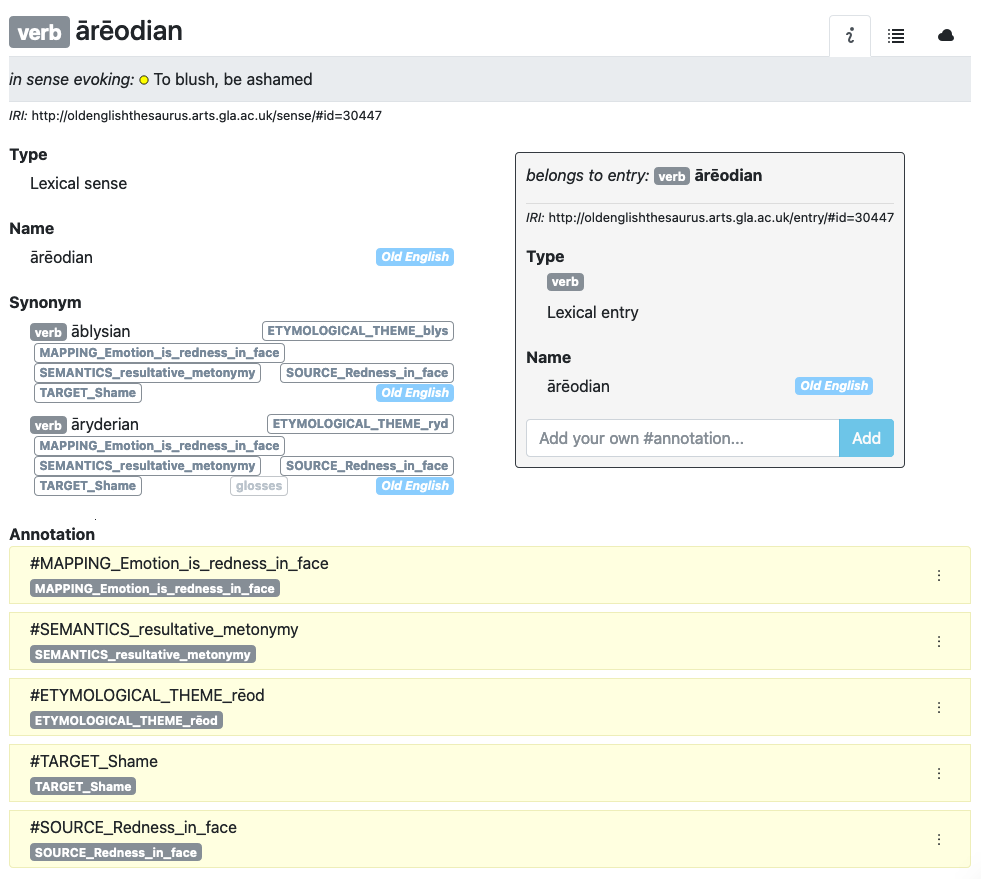
\includegraphics[width=\textwidth]{Stolk2021x/fig/Khan-areodian.png}
	\caption[]{\label{fig:Stolk2021x:Khan-fig1}A lexical sense annotated in Evoke with semantic mappings.}
\end{minipage}
\begin{minipage}{.04\textwidth}\end{minipage}
\begin{minipage}{.48\textwidth}
  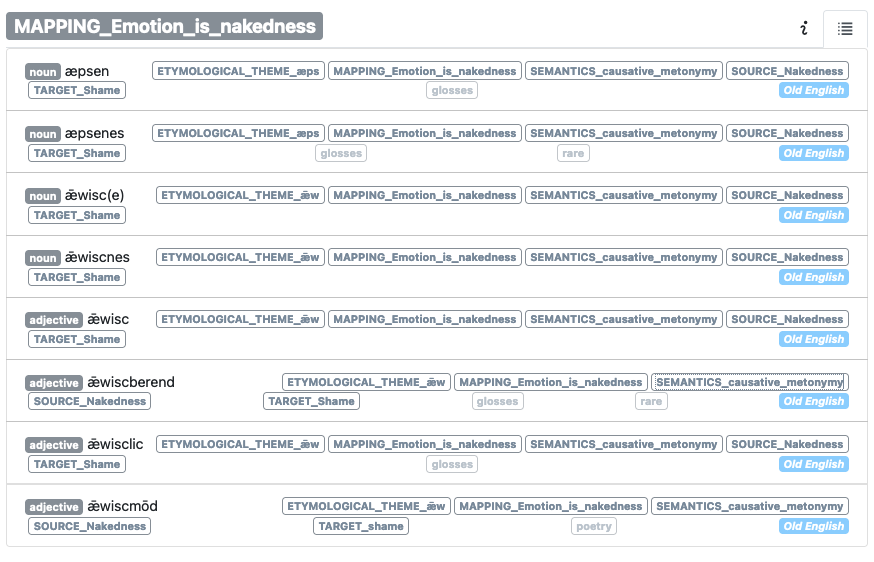
\includegraphics[width=\textwidth]{Stolk2021x/fig/Khan-metaphor-mapping.png}
	\caption[]{\label{fig:Stolk2021x:Khan-fig2}Overview in Evoke of senses with the metaphorical use \textsc{emotion is nakedness}.}
\end{minipage}
\end{figure}

As Khan et al. have demonstrated, thesauri are valuable resources for research on metaphors. Indeed, the value of these lexicographic resources for identifying and charting metaphorical relations between semantic fields has been reported in other research projects, too.\footnote{\textit{Mapping English Metaphor through Time}.} %\cite{MappingEnglishMetaphorThroughTime}. 
Additionally, Khan et al. revealed advantages to their having used Evoke. The annotation system of the application and the overviews generated offered the means to interact more closely with the source material. A thesaurus edition can thus not only be a source of information but %, instead of being completely separated from one's data management for research purposes, 
also act as a canvas for information produced. Such interaction with lexicographic resources may well facilitate feedback loops to provide the original editors with useful comments and suggestions that can be incorporated in revisions.





\section{Comparative analyses of Old Germanic languages}
\label{sect:Stolk2021x:cs-multilingual}

Two further EEMEE case studies demonstrated the value of thesauri for comparative analyses of related languages. The first, by Rita van de Poel and Sander Stolk, linked Old Frisian lexis with that of Old English captured in the \textit{TOE} dataset. The second case study, by Katrien Depuydt and Jesse de Does, connected Old Dutch to Old English. The resulting data connections provide an avenue of research for contrasting kindred languages through the overarching, onomasiological framework of the thesaurus. Thus, commonalities and differences between languages can emerge based on their %composition
representation of specific semantic fields.

\subsection{Old Frisian and Old English KINSHIP}
\label{sect:Stolk2021x:OldFrisianKinship}

The case study by Rita van de Poel and Sander Stolk used Evoke to link Old Frisian to Old English words captured by the \textit{TOE} dataset.\footnote{Van de Poel and Stolk, `A Case of Kinship'. The article in its entirety is included in this dissertation and follows the current chapter.} %\cite{doi:10.1163/18756719-12340239}.
In their work, the authors focused on the semantic field of \textsc{kinship} in the two related languages. In connecting Old Frisian lexis, drawn from a dictionary of Old Frisian, to the overarching structure of \textit{TOE}, the researchers created a dataset that positions Old English and Old Frisian lexis in the same semantic framework. The connected resources were shared and analysed using Evoke (see Figure \ref{fig:Stolk2021x:VanDePoel-fig1}).

\begin{figure}[h]
\centering
\begin{minipage}{.48\textwidth}
  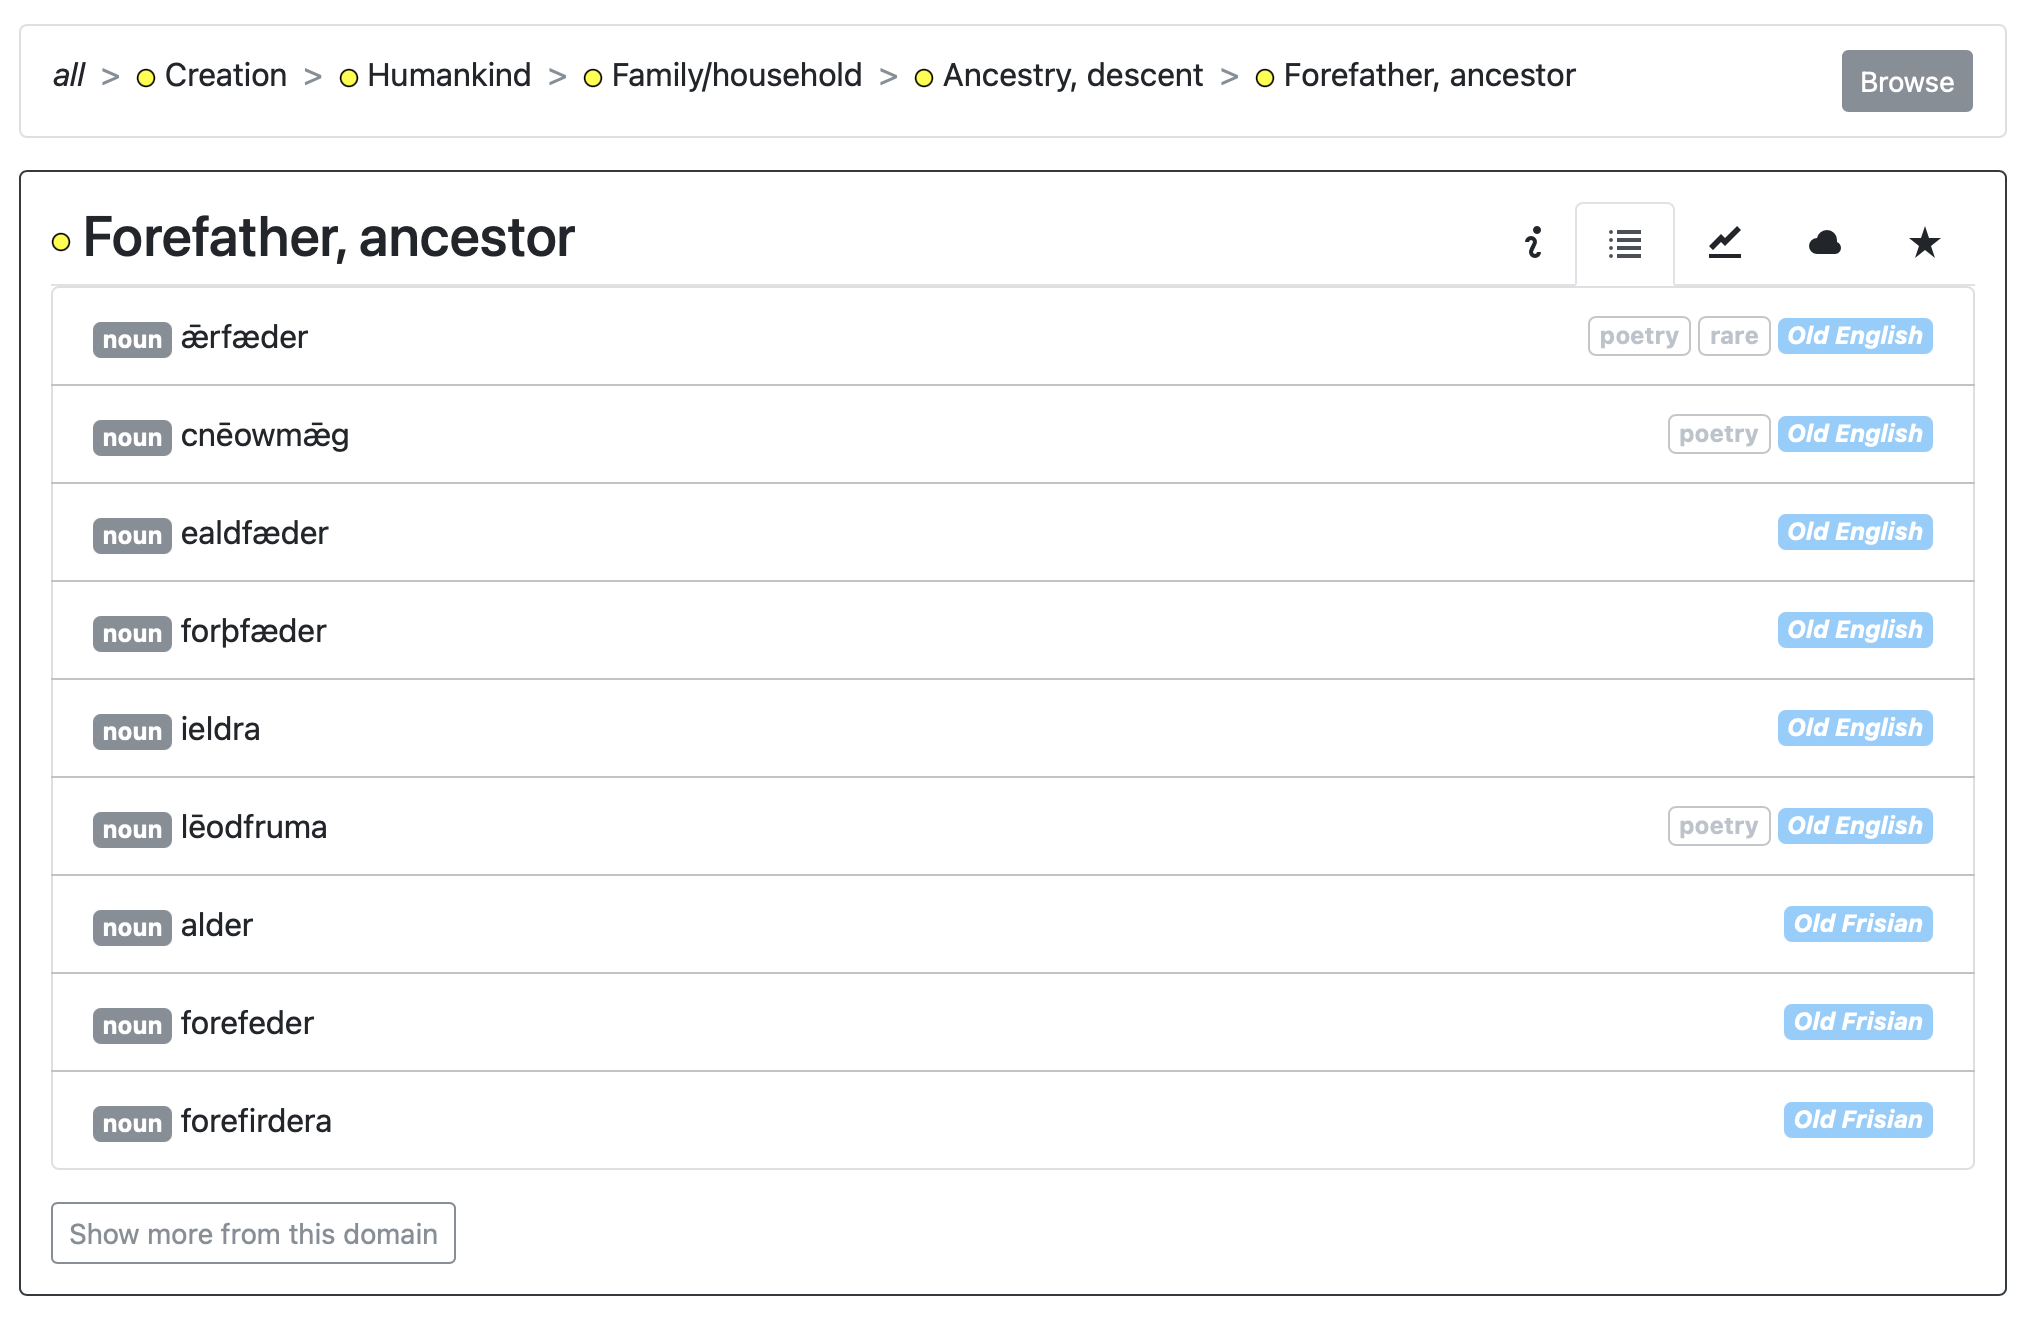
\includegraphics[width=\textwidth]{Stolk2021x/fig/VanDePoel-forefather.png}
	\caption[]{\label{fig:Stolk2021x:VanDePoel-fig1}An overview in Evoke of Old English and Old Frisian words denoting ``Forefather, ancestor''.}
\end{minipage}
\begin{minipage}{.04\textwidth}\end{minipage}
\begin{minipage}{.48\textwidth}
  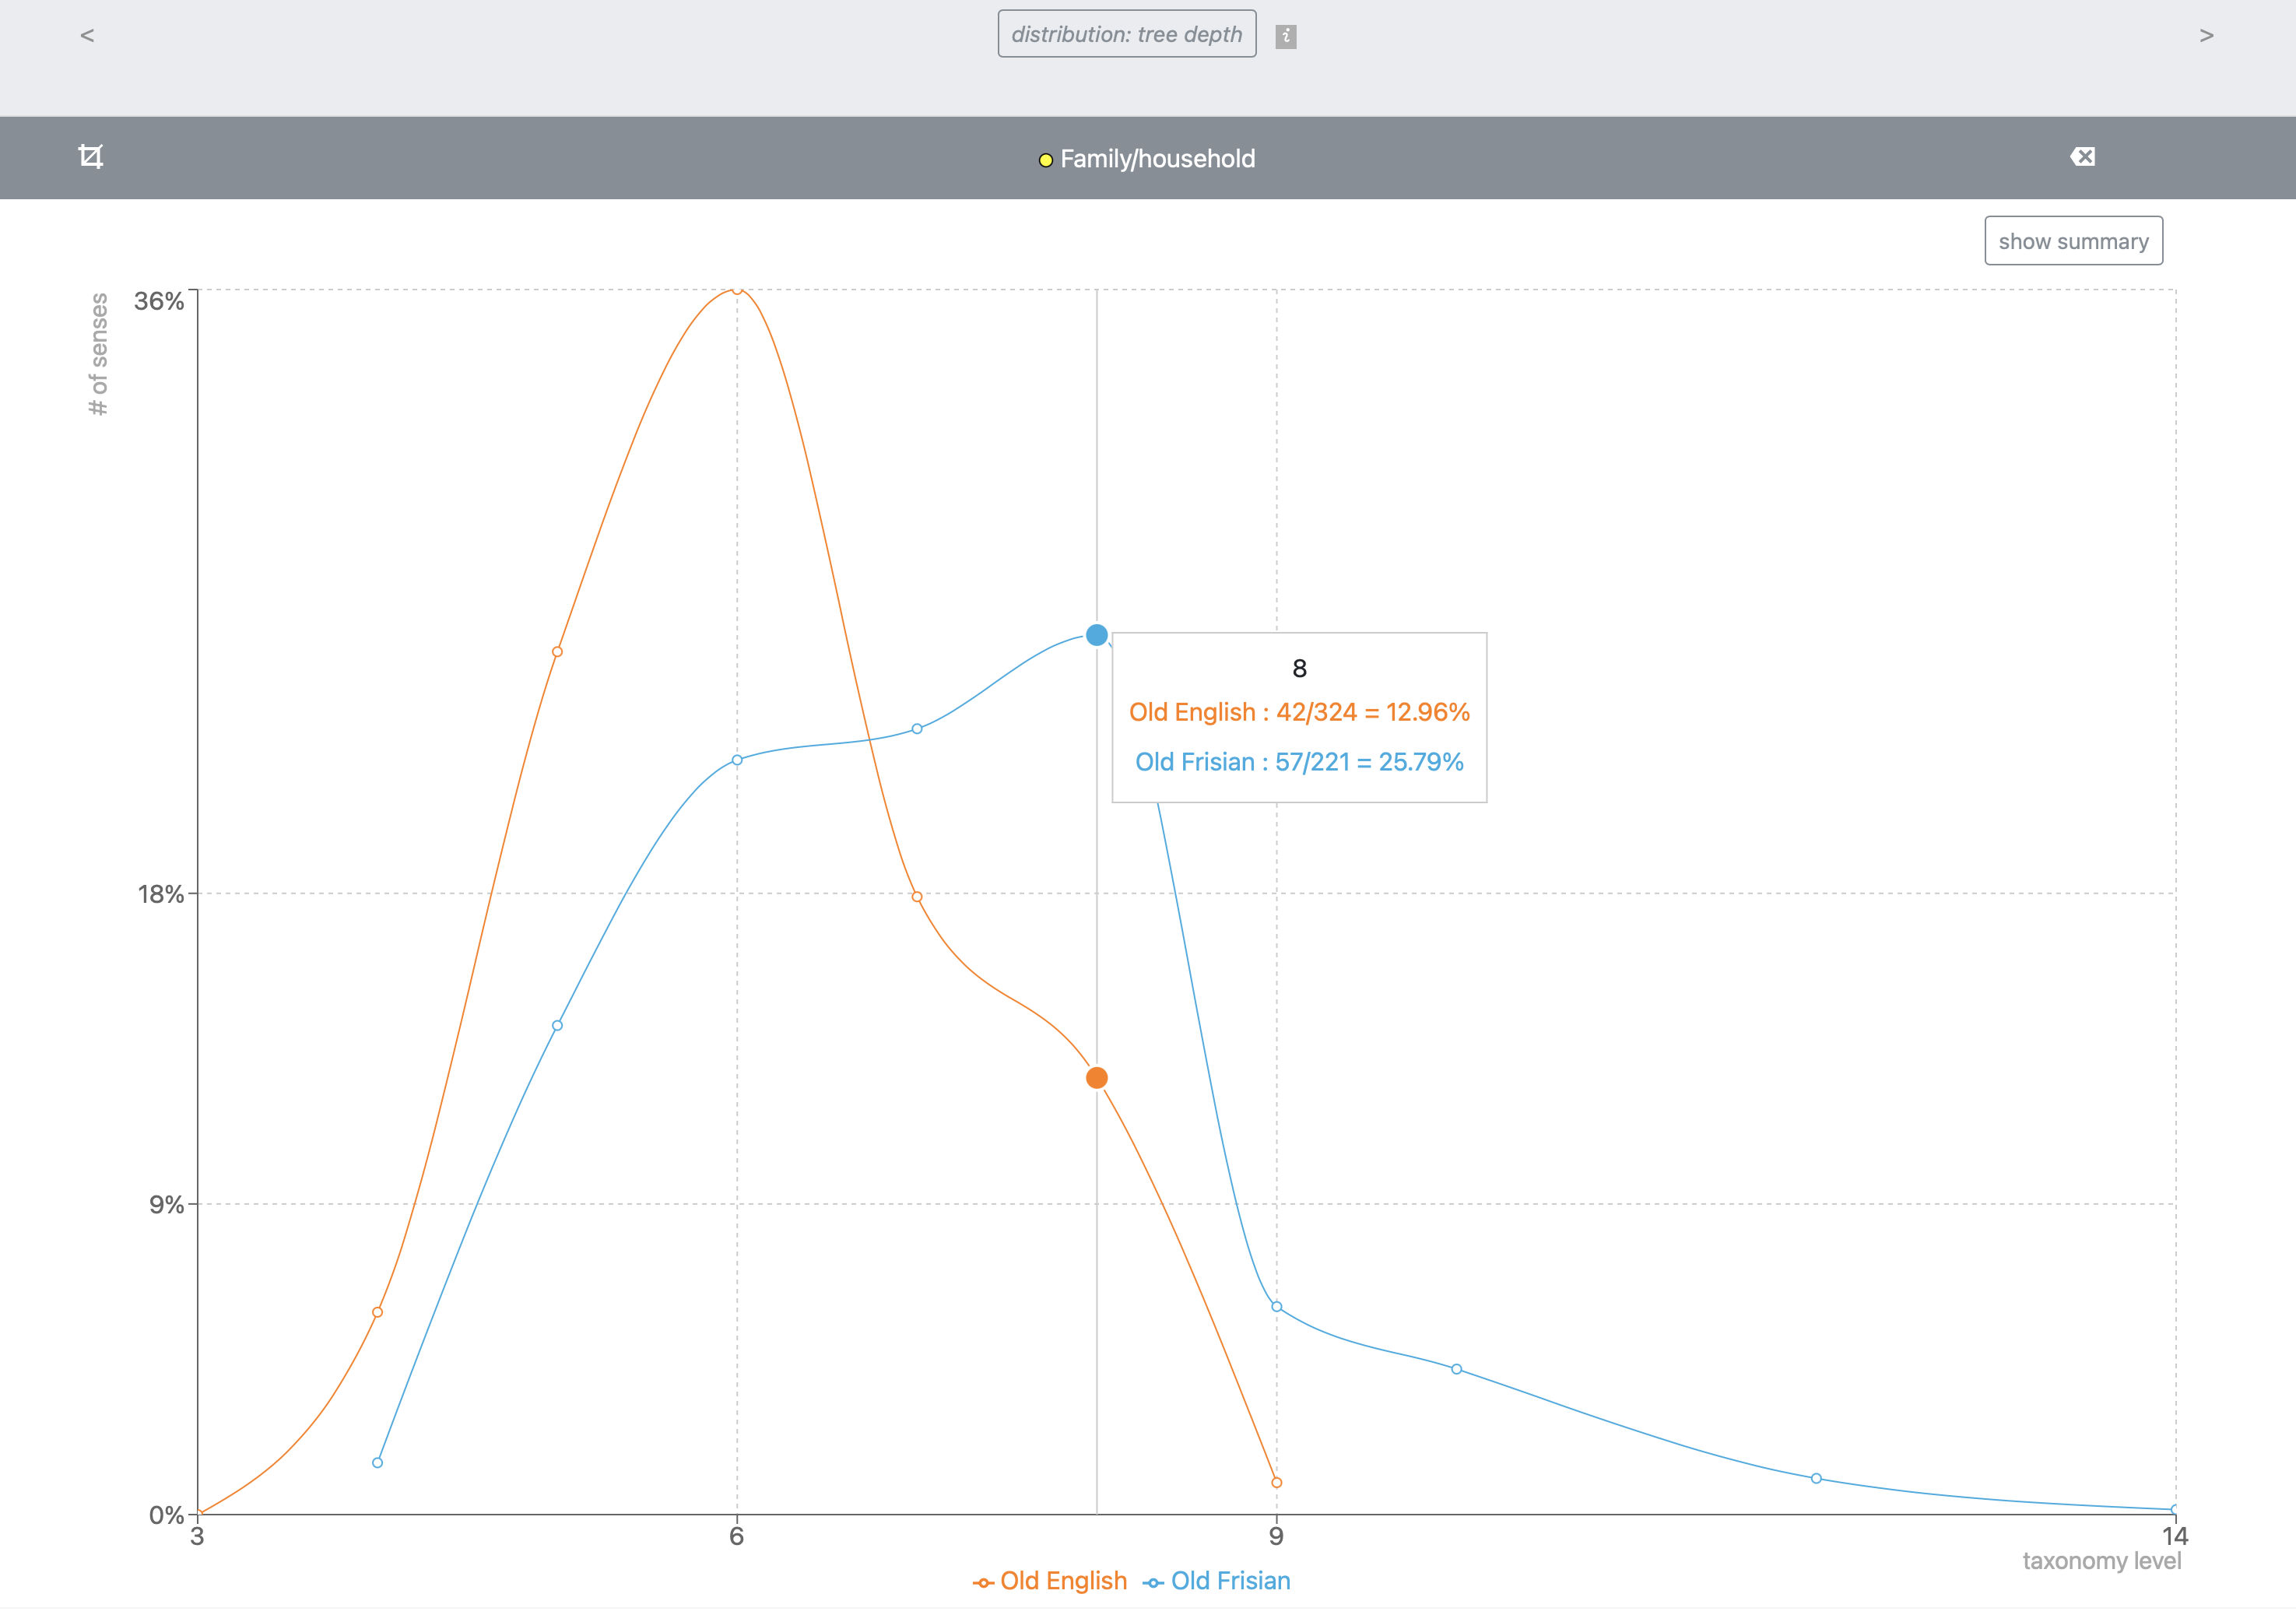
\includegraphics[width=\textwidth]{Stolk2021x/fig/VanDePoel-specificity.png}
	\caption[]{\label{fig:Stolk2021x:VanDePoel-fig2}Levels of specificity for Old Frisian and Old English \textsc{kinship}.}
\end{minipage}
\end{figure}

Van de Poel and Stolk demonstrated how Evoke facilitates comparative analyses between the two languages and argue that onomasiological analyses (such as shown in Figure \ref{fig:Stolk2021x:VanDePoel-fig2}) can uncover new linguistic and cultural insights. Their case study revealed how the two language communities conceptualized aspects relating to family, ancestry, descent, and adoption.\footnote{To illustrate, ``Adoption'' lacks Old Frisian senses entirely, whereas the concept of ``Siblings'' is lexicalized in this language but not in Old English (Ibid., p. 475).} 
Additionally, van de Poel and Stolk signaled that new thesauri can be created through adoption (and expansion) of the taxonomy of an existing thesaurus of a kindred language --- one semantic field at a time. 
Evoke and the Linguistic Linked Data paradigms support such endeavours, as they allow researchers to access and extend \textit{TOE} data whilst abiding by the license of the thesaurus, which restricts users from extracting or downloading substantial portions of the dataset.

In addition to presenting their findings, van de Poel and Stolk shed light on the major hurdles and limitations in connecting material from two lexicographic resources and analysing the results.\footnote{Ibid., p. 477.} 
Comparisons such as theirs, they note, are influenced by differences in lexicographic practices and editorial choices. The editors of \textit{TOE} and those of the dictionary of Old Frisian will have had, or worked with, different approaches towards the granularity of word senses to include.\footnote{The practice of maintaining only generic word senses is not uncommonly referred to as lumping, whereas distinguishing fine-grained senses is termed splitting (see Fontenelle, `Bilingual Dictionaries', pp. 45-6; Kay and Alexander, `Diachronic and Synchronic Thesauruses', p. 370).} Additionally, positioning the Old Frisian lexis in \textit{TOE} categories was complicated by the use of different languages for the sense definitions (i.e., English in \textit{TOE} versus German for the Old Frisian lexis). Nevertheless, the researchers found ways to overcome these issues and succeeded in aligning the two lexicographic resources, thereby adopting the overarching structure of \textit{TOE} as a comparative framework for the two related historical languages. Thus, the scholars could avoid fashioning an onomasiological structure for Old Frisian from the ground up and subsequently, prior to analysis, attempting to reconcile it with that of \textit{TOE}. The resulting, combined dataset allows researchers of both Old Frisian and Old English to adopt the same structure and to identify and discuss notable differences in conceptualizations between the kindred languages through shared semantic domains. 

\subsection{Linking Old Dutch to Old English}

Katrien Depuydt and Jesse de Does took a more technical route than Rita van de Poel and Sander Stolk towards linking lexis from another language to \textit{TOE}.\footnote{Depuydt and de Does, `Linking the \textit{Dictionary of Old Dutch} to \textit{A Thesaurus of Old English}'.} In their case study, they reflected on their experiments with manual and automatic techniques in order to establish connections between entries from the \textit{Dictionary of Old Dutch} and the \textit{TOE} dataset available in Evoke. In doing so, they investigated whether the existing macrostructure of \textit{TOE} can be reused to create a thesaurus of Old Dutch. %Depuydt and De Does outline the possibilities and potential pitfalls involved in such an endeavour.

Their research compared two approaches to linking the two lexicographic resources. The first approach was a manual one, in which the tool Lex'it was used to view entries of Old Dutch words and record appropriate categories from the \textit{TOE} hierarchy for their registered senses (see Figure \ref{fig:Stolk2021x:Depuydt-fig1}). Additional matches were obtained by drawing on cognate information. Cognate relations of Old Dutch entries were traversed to Old Frisian ones that had already been linked to \textit{TOE} categories (based on the work by van de Poel and Stolk described in section \ref{sect:Stolk2021x:OldFrisianKinship}). The second approach explored by the authors was semi-automated linking, where five different matching algorithms were contrasted and evaluated. Depuydt and de Does concluded that further directions for linking such lexicographical resources may be found in improving automated linking techniques, crowdsourcing part of the process, and improving visualization of candidate links for verification purposes.

\begin{figure}[h]
    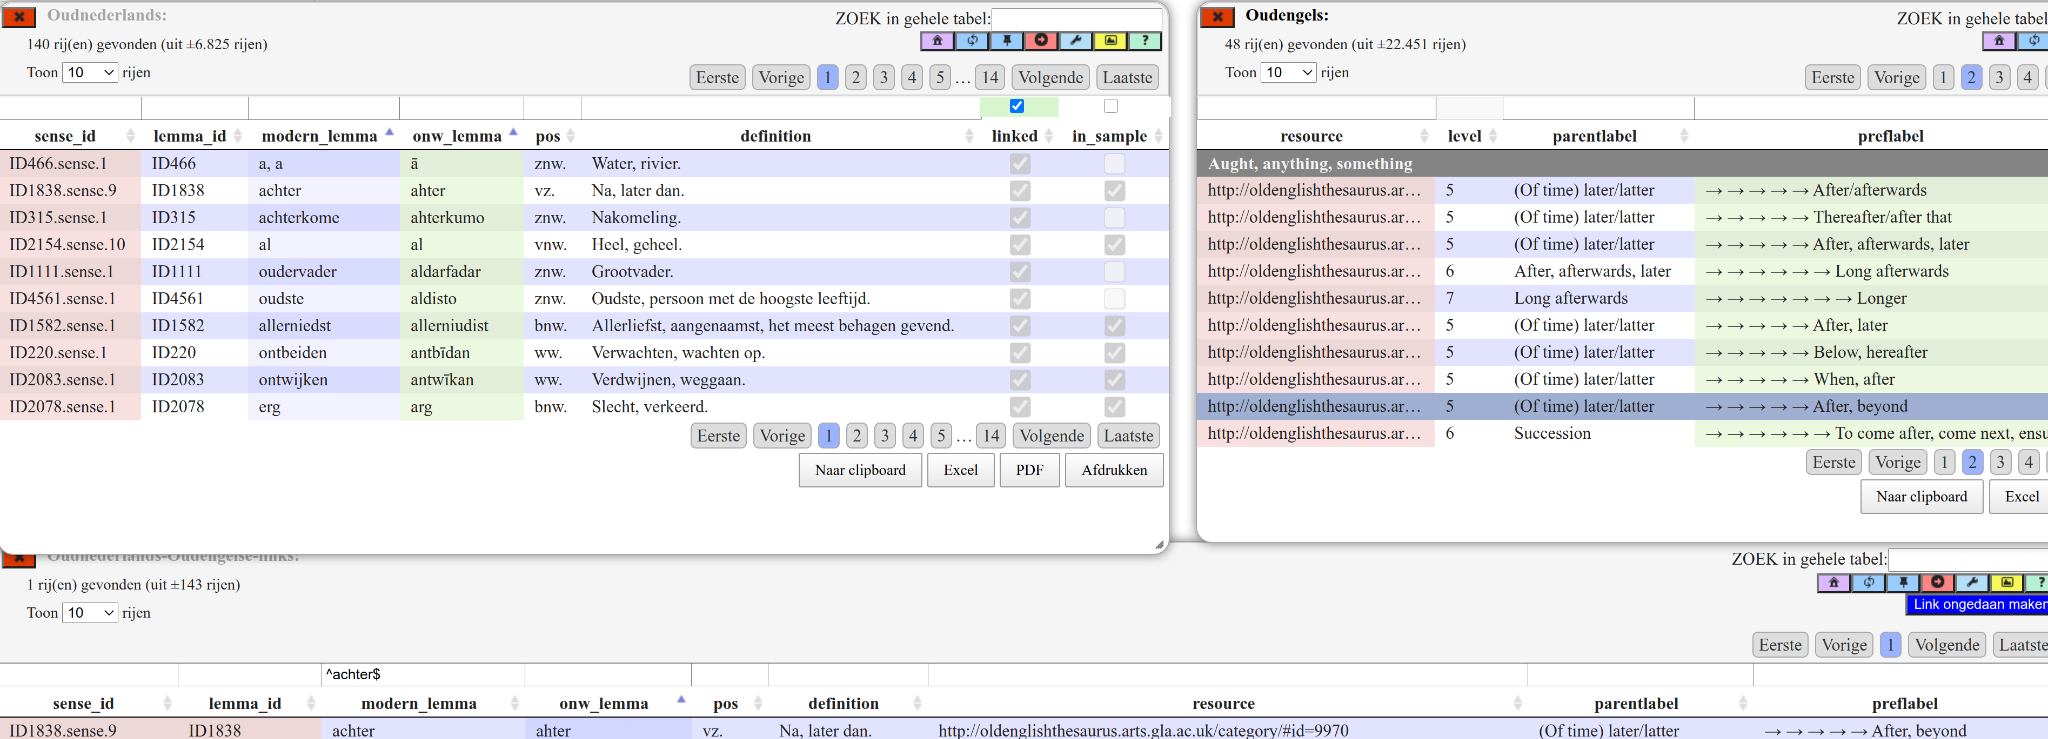
\includegraphics[width=\textwidth]{Stolk2021x/fig/Depuydt-lexit-b.png}
	\caption[]{\label{fig:Stolk2021x:Depuydt-fig1}The Lex'it-based linking tool; linking the entry for Old Dutch \textit{ahter} to the \textit{TOE} category ``05.11.07.04.02|13 (Of time) later/latter: After, beyond''.}
\end{figure}

The case study demonstrated two key advantages of the Linguistic Linked Data form in which \textit{TOE} has been made available. Firstly, connections between Old Dutch lexis and \textit{TOE} categories could be established and stored separately from the \textit{TOE} dataset. This possibility ensures that researchers other than the editors of \textit{TOE} can extend the semantic framework formed by the thesaurus, even when they do not have direct access to the raw data of the thesaurus or to the database in which it is stored. Secondly, information linked in previous research could be queried alongside the original thesaurus material and, thus, drawn on for analyses. In this case, the Old Frisian lexis for \textsc{kinship}, positioned in thesaurus categories by van de Poel and Stolk (see \ref{sect:Stolk2021x:OldFrisianKinship}), could be combined with cognate information and leveraged for positioning Old Dutch lexis within the onomasiological structure of the thesaurus.

% TP: Yes, OK, but these are advantages of the LLD format and are not specific to the comparative analyses discussed here. If I were you, I would focus on the fact that Evoke allows an established macrostructure/onomasiological framework, such as the one established by TOE, to be RE-USED for the lexis other languages  and that using the same macrostructure/onomasiological framework facilitates important comparative research. Of course, then there is the question of whether it is unproblematic to re-use the same macrostructure, for two different languages in their entirety, to which the answer is a 'no' if we go by Depuydt and De Does, but Van de Poel and Stolk show that it can be very effective for a selected group of semantic fields?
A dataset containing the established connections between the Old Dutch dictionary material and \textit{TOE} has been made available on a webpage dedicated to the case study.\footnote{\url{https://ivdnt.org/corpora-lexica/diamant/onw-toe-linking/}} The availability of this dataset enables researchers to perform comparative analyses of Old Dutch and Old English. In their article, Depuydt and de Does do not yet include such an analysis. Their insights on the reuse of an existing onomasiological framework -- i.e., that of \textit{TOE} -- are therefore limited to the difficulties encountered in creating suitable connections. The language-specific nature of \textit{TOE}, built as it was for ``fitting the intricacies of Old English lexis'', is one of the reasons the authors put forward for the complexity of matching items from other languages.\footnote{Depuydt and de Does, `Linking the \textit{Dictionary of Old Dutch} to \textit{A Thesaurus of Old English}', p. 509.} Additionally, an unfamiliarity with the structure of the thesaurus can impede locating the categories that are of interest. Indeed, Depuydt and de Does indicate that manually assigning Old Dutch lexis to suitable categories within the onomasiological structure of \textit{TOE} was hampered for this reason.\footnote{Ibid., p. 510.} %hindered the process of manually locating suitable categories within that structure to which Old Dutch lexis ought to be assigned.
Therefore, studies that are sizable in scope may warrant gaining an intimacy with the topical system of a thesaurus before adopting it for other languages and comparative analyses.



\section{Teaching Old English language and culture}
\label{sect:Stolk2021x:cs-teaching}

The last aspect of historical language thesauri explored in EEMEE was their didactic potential. Kees Dekker, at University of Groningen, and Thijs Porck and Sander Stolk, at Leiden University, employed \textit{TOE} and Evoke to introduce students to notable aspects of Old English language and culture. In both cases, Bachelor students were asked to discern nuances within semantic domains and theorize as to how these might reflect the culture of the Anglo-Saxons. The outcome of the experiment was that students were shown to benefit from extensive use of these resources throughout a course, as is the case with University of Groningen, but also from more concentrated use, such as in workshops at Leiden University. Experiences of the two universities are treated below in separate sections.

\subsection{The Old English classroom at University of Groningen}

%The last contribution to this special issue looks at the didactic potential of \textit{TOE} and Evoke.
In his case study, Kees Dekker employed \textit{TOE} and Evoke in a classroom context through a series of increasingly complicated search assignments.\footnote{Dekker, `Evoke and \textit{A Thesaurus of Old English} in the Old English classroom'.} %\cite{doi:10.1163/18756719-12340241} 
These assignments, intended to interest, challenge, and instruct students, were preceded by an introduction into lexical semantics to inform students of such notions as semantic fields, hyponymy, and synonymy --- notions at the core of \textit{TOE} and other thesauri. 
During a seven-week module, students received assignments on \textit{TOE} and Evoke that were related to the Old English texts they were asked to read and translate. The assignments ranged from, at the start of the module, navigating the thesaurus to take note of the lexis and distinctions available for bodies of water (see Figure \ref{fig:Stolk2021x:Dekker-fig1}) to, at a more advanced stage, questioning the notion of `foreign' in Old English (see Figure \ref{fig:Stolk2021x:Dekker-fig2}) by discerning what the early medieval speakers of this language considered foreign and what connotations their words for this concept had. Through his discussion of both the assignments for students and their responses, Dekker demonstrated that Evoke is a valuable addition to a teacher's tool set, as it invites students and researchers alike to explore Old English in novel and interesting ways.

\begin{figure}[h]
\centering
\begin{minipage}{.48\textwidth}
  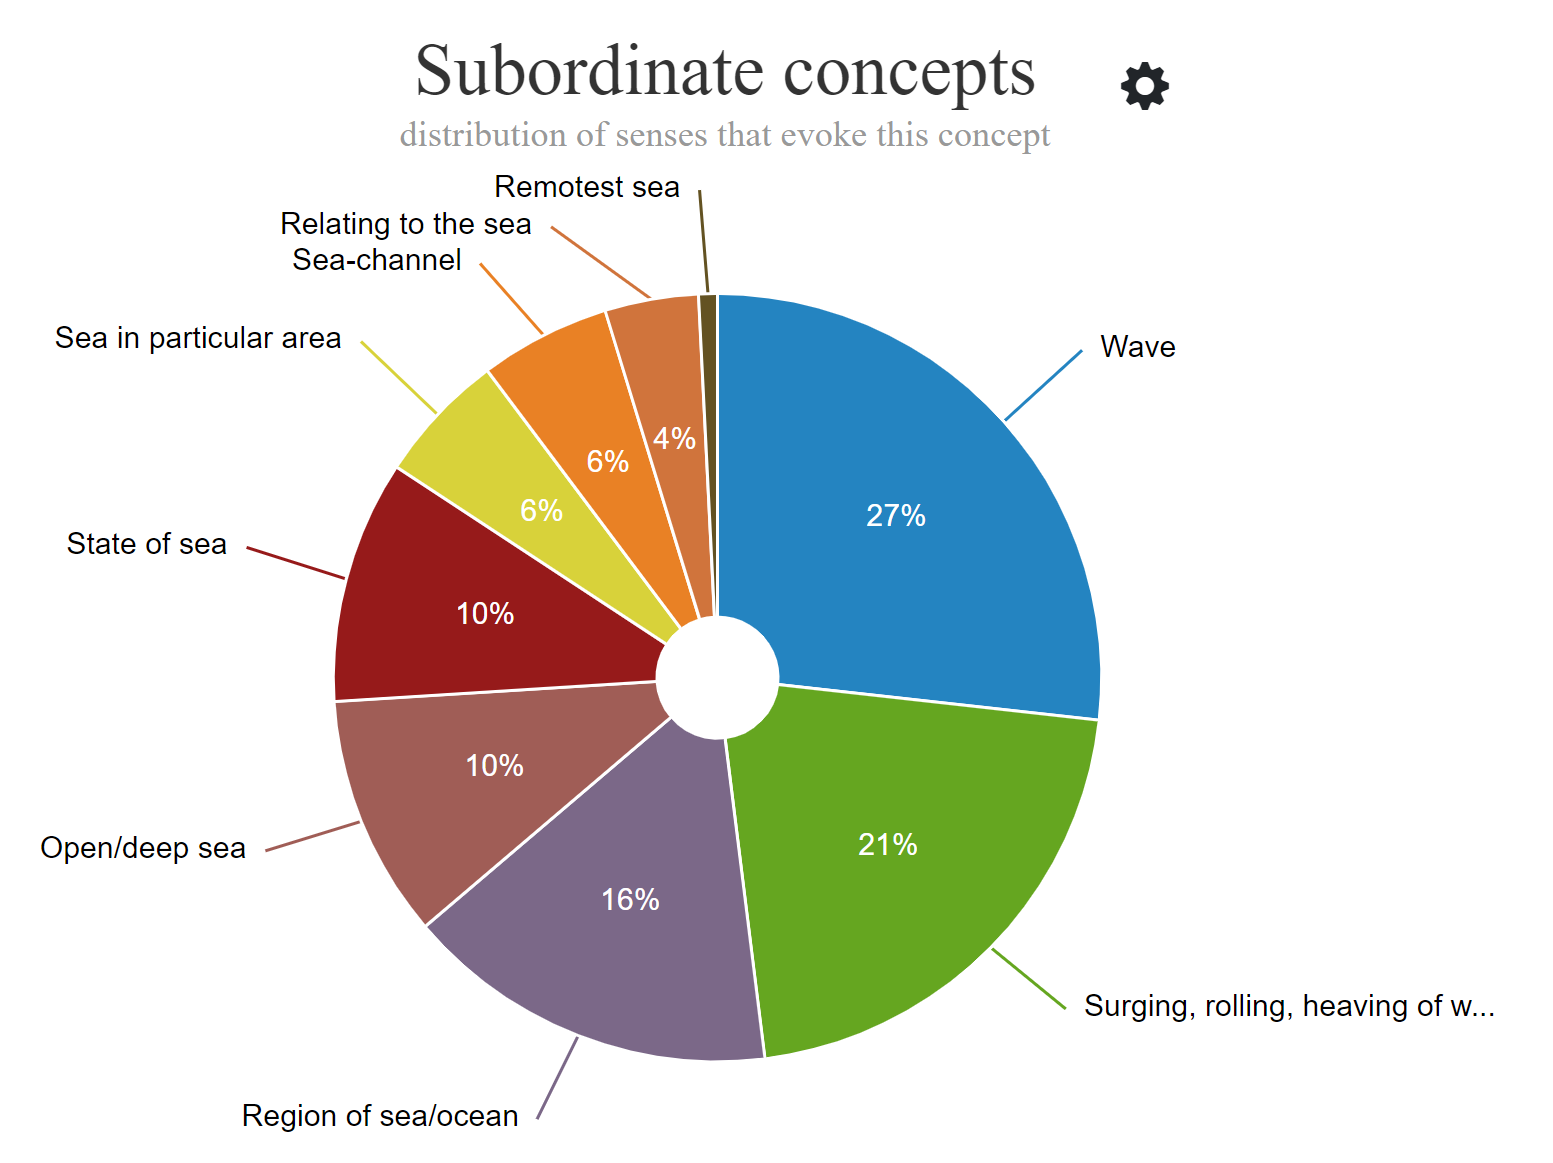
\includegraphics[width=\textwidth]{Stolk2021x/fig/Dekker-sea-ocean.png}
	\caption[]{\label{fig:Stolk2021x:Dekker-fig1}Pie chart in Evoke showing the distribution across the subordinate concepts of the \textit{TOE} category ``Sea/ocean''.}
\end{minipage}
\begin{minipage}{.04\textwidth}\end{minipage}
\begin{minipage}{.48\textwidth}
  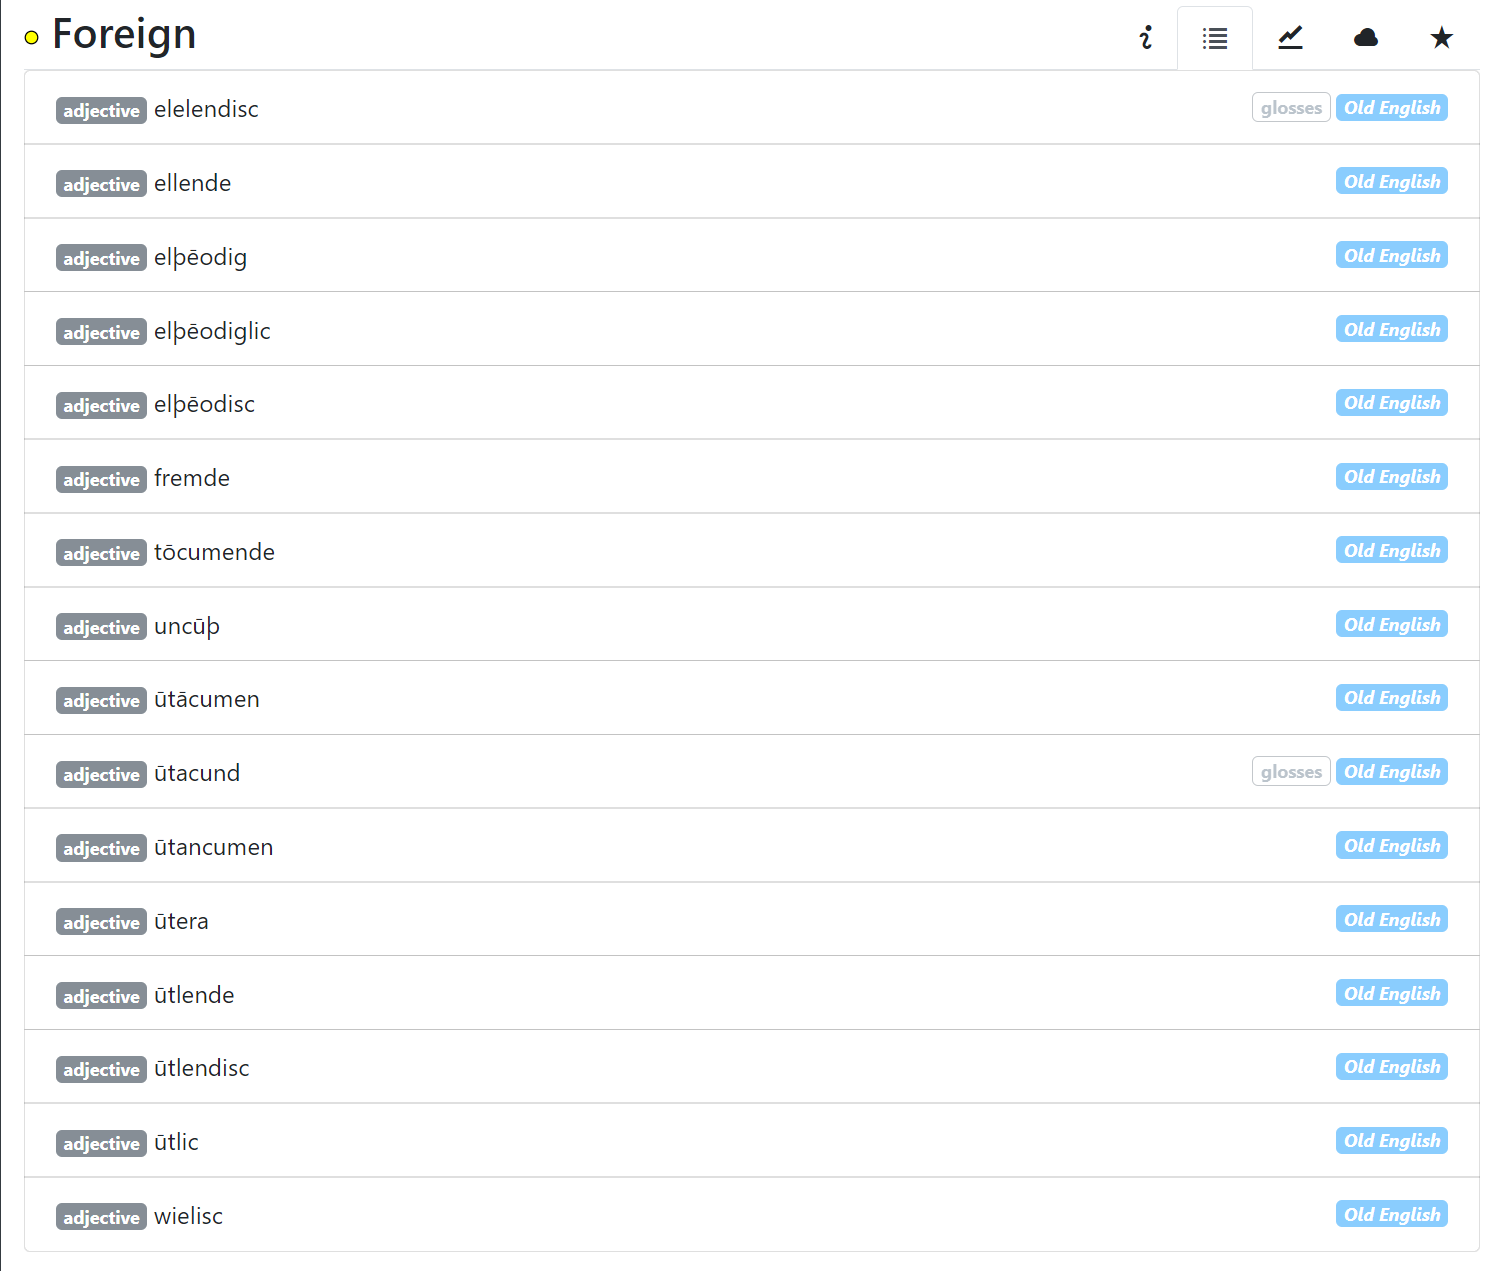
\includegraphics[width=\textwidth]{Stolk2021x/fig/Dekker-foreign.png}
	\caption[]{\label{fig:Stolk2021x:Dekker-fig2}List of Old English words in Evoke denoting ``foreign''.}
\end{minipage}
\end{figure}

Although the requirements for Evoke were formulated to support research first and foremost,\footnote{Stolk, `Evoke'.} %\cite{doi:10.1163/18756719-12340235}
Dekker's article demonstrates that the design of the web application enables students, too, to explore a thesaurus and engage with the lexical material presented. The functionality to navigate and view thesaurus material supports users without expertise or prior knowledge of Linguistic Linked Data or thesauri. Moreover, the many visualizations included in Evoke allow students to engage with the material in a playful manner: Next to pie charts, which provide statistics beneficial to research, wordcloud visualizations of entire semantic fields (see Figure \ref{fig:Stolk2021x:Evoke-wc}) have led to students calling Evoke ``fun'' as well as ``useful'' (see Appendix \hyperref[Appendix8.C]{8.C}, Table \ref{table:Stolk2021x:eval:Evoke-overall}). 

\begin{figure}[h]
\centering
\begin{minipage}{.48\textwidth}
  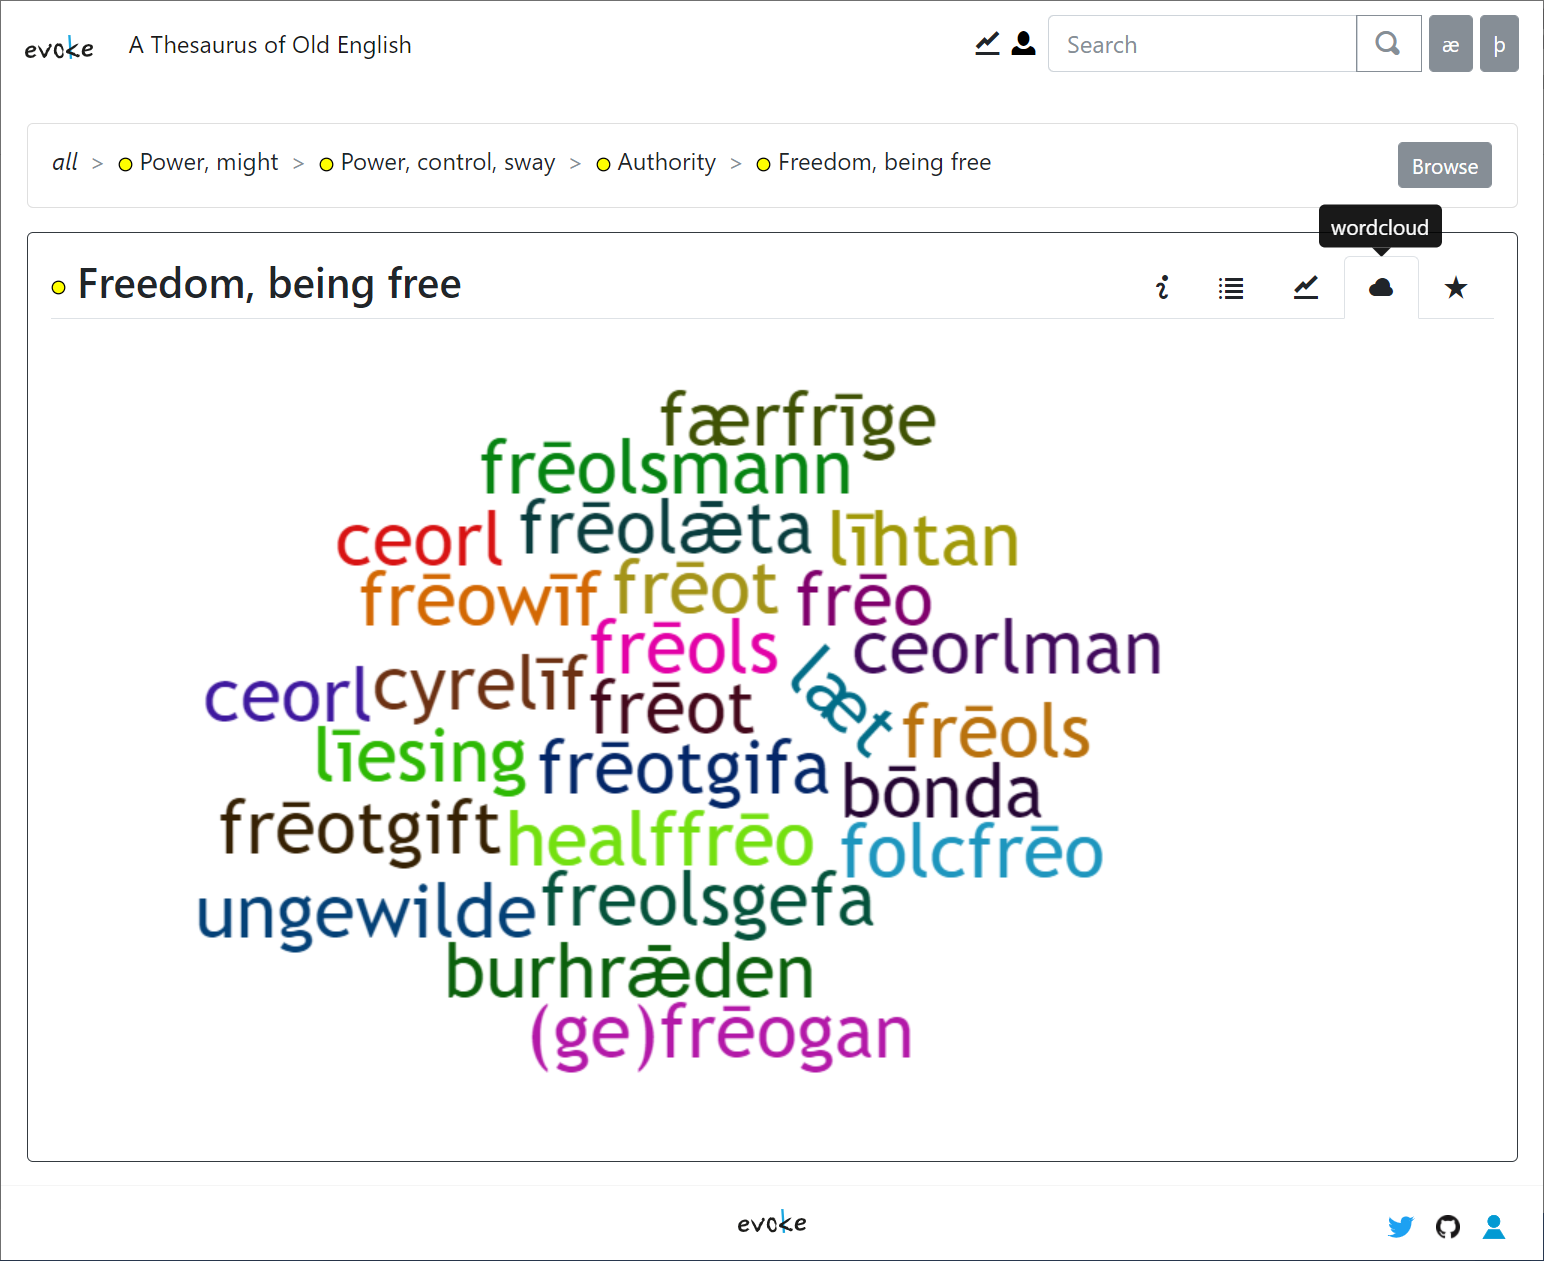
\includegraphics[width=\textwidth]{Stolk2021x/fig/Stolk-wordcloud.png}
	\caption[]{\label{fig:Stolk2021x:Evoke-wc}Wordcloud in Evoke for ``Freedom, being free''.}
\end{minipage}
\begin{minipage}{.04\textwidth}\end{minipage}
\begin{minipage}{.48\textwidth}
  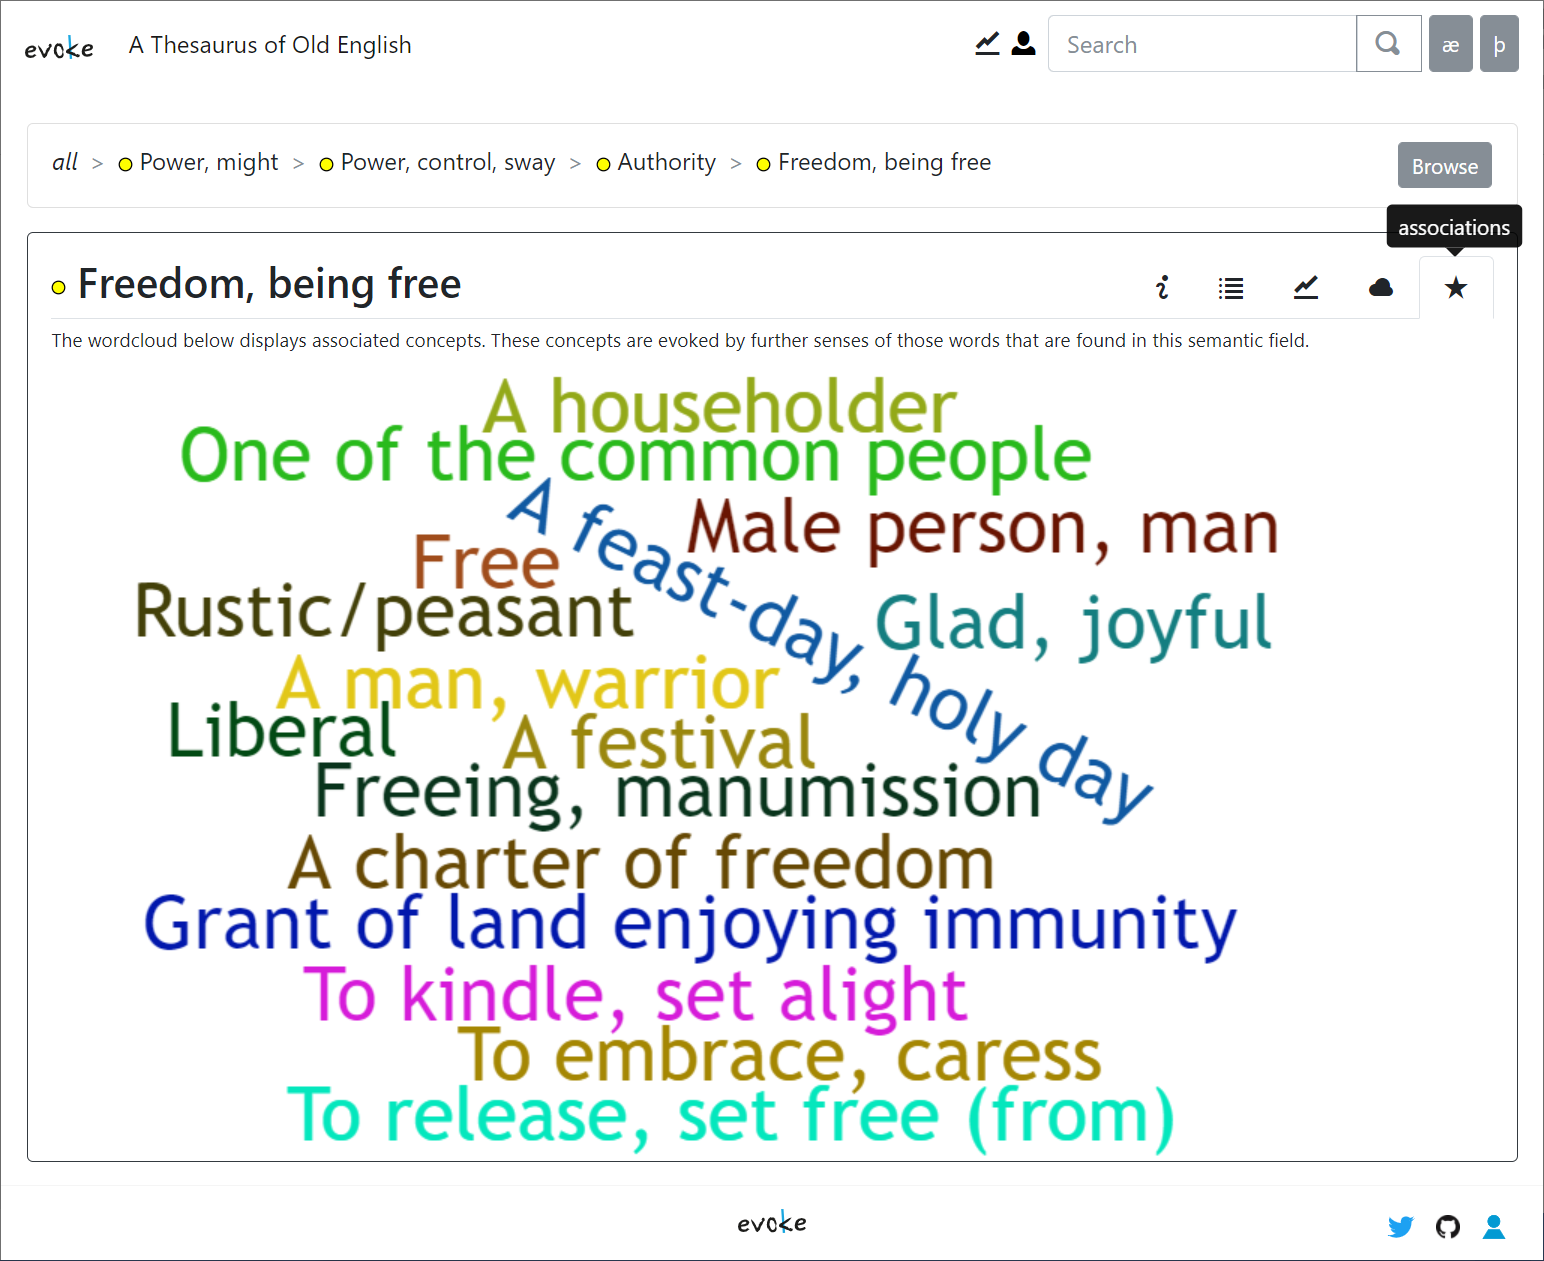
\includegraphics[width=\textwidth]{Stolk2021x/fig/Stolk-associations.png}
	\caption[]{\label{fig:Stolk2021x:Evoke-assoc}Associations in Evoke for ``Freedom, being free''.}
\end{minipage}
\end{figure}


For future use of Evoke in educational settings, Dekker points out that, although already valuable, the web application could be improved by incorporating ``a repository of questions and assignments shared by instructors interested in the use of Evoke for curricular and research purposes''.\footnote{Dekker, ‘Evoke and A Thesaurus of Old English in the Old English classroom’, p. 526.} Such an addition is indeed already planned. Existing teaching material will be incorporated in the Evoke website. Preliminary work has been done towards its realisation. By courtesy of Prof. Carole Hough (University of Glasgow), the exercises will include units from the module \textit{Learning with the Online Thesaurus of Old English}.%\cite{LearningWithTOE}.


\subsection{Workshops on Old English resources at Leiden University}

Dekker's findings on the use of Evoke in education are reinforced by those at Leiden University, where the web application has been used in a classroom setting, annually, since 2018. Third-year Bachelor students perform a number of assignments in Evoke during a 2-hour workshop on digital tools and resources for studying Old English, led by Thijs Porck and Sander Stolk. The first of these workshops, which took place on 13 November 2018, included an evaluation by students of the application (see Appendix \hyperref[Appendix8.C]{8.C}). Students considered navigation in Evoke to be ``clear'' and ``easy'' to understand. Moreover, views and analyses offered by the application enabled them to obtain results to the following questions, amongst others, in an ``efficient'' manner:
\begin{quote}
    How many words does Old English have for Hell and its subcategories? How about for Heaven?
\end{quote}
\noindent The statistics tab in Evoke provides exactly such figures at a glance, avoiding the need for students and researchers to manually count the words listed under various categories.

A recurring element in assignments for students at both Leiden University and University of Groningen has been to establish connotations of words or semantic fields in their entirety. A case in point is the following illustrative question: 
\begin{quote}
    The \textit{TOE} lists several words for old age, including \textit{gelefed} `old', \textit{har} `old' and \textit{frod} `old'. Find out what else these words mean. Search for ``gelefed'', ``har'' and ``frod''. What, according to your findings, did the Anglo-Saxons associate with old age?
\end{quote}
\noindent Students viewed each word listed separately to ascertain their various senses and, thus, indications of connotations of words used in a certain meaning. During the second EEMEE workshop, it became clear that obtaining connotations of an entire semantic field is deemed valuable for education purposes but, with the then available functionality of Evoke, still required students to engage with content in this piecemeal fashion. A new visualization was therefore introduced. The `associations' wordcloud, available since version 1.4.1 of Evoke, provides an overview of all senses in a semantic field related through polysemy (see Figure \ref{fig:Stolk2021x:Evoke-assoc}). In short, feedback on the use of Evoke and \textit{TOE} in education has been valuable in informing the development of Evoke.


\section{Discussion}
\label{sect:Stolk2021x:discussion}

This section discusses the usefulness of the digital resources at the heart of the case studies presented above: 
%The case studies presented in this chapter warrant a discussion on the usefulness of the digital resources at their heart: 
the Linguistic Linked Data form of \textit{TOE} and the web application Evoke. Both resources have been developed specifically for facilitating research, which raises the question in what manner, if any, they have enabled new lines of scholarly enquiry compared to existing editions of historical language thesauri. %This section will discuss each resource separately, starting with the new digital form in which \textit{TOE} has been captured.

\subsection{\textit{A Thesaurus of Old English} as Linguistic Linked Data}

The Linguistic Linked Data form of \textit{TOE} (or \textit{TOE}-LLD), as made available in Evoke, enabled researchers to extend the original dataset of the thesaurus with information salient to their inquiries. In contrast to many existing editions of historical language thesauri of Scots and English, this digital form includes unique identifiers (IRIs) for lexical items as well as categories.\footnote{To illustrate, \textit{HTE} does not issue IRIs for a specific lexical sense. The search hit \textit{strength} as found at category ``02.02.06.01|06 (n.) Strength of evidence'', for example, refers to the following subpath on the \textit{HTE} website: \url{/category/?id=123117&qsearch=strength}. This web address indicates that  category 123117 is to be shown, i.e., ``Strength of evidence'', whilst highlighting any text that matches the string `strength'. The web address is therefore not an exact reference to the specific item requested, but a visual aid that potentially foregrounds other entries, too, that include the aforementioned string. For further information on IRIs, see Chapter 3.} These identifiers have facilitated explicit references and, in the case of \textit{TOE}-LLD, are unaffected by potential modifications to the spelling of the headword. Being able to reference, view, and link information to lexical items has proven valuable for research in the case studies described above. Moreover, the inclusion of lexical entries in \textit{TOE}-LLD allows researchers to mark items of interest more broadly than per individual lexical sense (cf. the case study by Thijs Porck). 
These entries, deduced automatically from contextual information available in the original \textit{TOE} dataset, may still need manual revision in places: some homonyms have been lumped together and senses of lexemes remain ungrouped when their headwords use inconsistent spelling or grammatical forms.\footnote{See Porck, `Onomasiological Profiles of Old English Texts', p.366.} To eliminate the inherent caveats of such an automated process, thesaurus editors may wish to maintain lexical entries explicitly in order to facilitate these research needs.

Another important advantage in adopting IRIs is that their use simplified extending \textit{TOE} content without having access to the raw data of the thesaurus. Scholars were able to capture knowledge and, in their data, include explicit references to information found in \textit{TOE}-LLD. This capability is advantageous for research, since the license of \textit{TOE} prohibits users from downloading large amounts of thesaurus data.\footnote{See \textit{TOE4}, section `Copyright and Conditions of Use'.} Licenses that restrict access in such a manner are not uncommon for lexicographic resources available on the Web.\footnote{See, for instance, \textit{Oxford English Dictionary Online}, \textit{HTE}, and the historical Dutch dictionaries part of the \textit{Geïntegreerde Taalbank}.} The \textit{TOE}-LLD version thus lowers the barrier for scholars to engage with the available material.

\begin{comment}
Perceived benefits in using this data form are mentioned by Christian Chiarcos et al.\footnote{Chiarcos et al., `Towards Open Data for Linguistics: Lexical Linked Data'.} One of these benefits is the ability to merge different datasets, or relate different perspectives and conceptualizations of similar data, in order to obtain a combined set of data that is validly formatted. Thus, thesauri and sets of data elaborating on them can be queried in unison.\footnote{This capability facilitates extending original thesaurus content (see requirement R3 in Chapter 2).} A second benefit is an increased level of interoperability. Using standardized terminology in describing linguistic data increases a shared understanding of that data and facilitates their interpretation by software. Moreover, the use of IRIs as identifiers ensures data can be linked without the need for duplication of information from one set into another. The ability to link (or reference) in such a manner is valuable for historical language thesauri, too, since some of these resources are subject to licenses meant for viewing only, stipulating that users are not allowed to copy or download a substantial portion of their content (e.g., \textit{TOE} and \textit{HTE}). By adopting IRIs in published thesauri, their users should be able to explore and extend these resources, engaging with the content offered, without infringing on such licenses.
\end{comment}

In addition to the usefulness of IRIs for linking data, even when restrictive licenses are in place, Christian Chiarcos et al. claim two further benefits to use of Linguistic Linked Data.\footnote{Chiarcos et al., `Towards Open Data for Linguistics: Lexical Linked Data'.} The first is an increased level of interoperability owing to the reuse of established data vocabularies (i.e., Lemon-OntoLex and SKOS).\footnote{See Chapter 3.} Improved interoperability manifests itself in the shape of software other than Evoke being able to operate on the same data and/or data form. Examples of tools used in the various case studies include custom alignment tools, Microsoft Excel, and Lex'it.\footnote{These tools are described in Chapter 6, section 4.3.2, `Linking Data'. The \hyperref[fm:sourcecode]{`List of source code'} in the back matter of the dissertation includes relevant links to code developed for software applications and data transformations, which includes the custom alignment tools.} 
%To illustrate by means of the case studies presented here: Porck employed a custom alignment tool to enrich \textit{TOE}-LLD; Van de Poel and Stolk employed OpenRefine to transform content in Excel spreadsheets to Linguistic Linked Data; and Depuydt and De Does utilized the tool Lex'it.\footnote{The first two tools are described in Chapter 6, section 4.3.2, `Linking Data'. The List of Source Code in the front matter of the dissertation includes relevant links to code developed for software applications and data transformations. Lex'it is described more fully in the article by Depuydt and De Does referred to in this chapter.} 
Compatible software beyond those employed in the case studies exists, too. Cases in point are VocBench 3 and LexO, with which users can fashion and maintain such data.\footnote{Stellato et al., `VocBench 3'; Bellandi and Giovannetti, `Involving Lexicographers in the LLOD Cloud with LexO'.} Current endeavours with Linguistic Linked Data suggest an uptake of this digital form and tools that can operate on it over the next few years. These include the H2020 projects ELEXIS (2018–22), Prêt-à-LLOD (2019–22), and the COST Action NexusLinguarum (2019–23).\footnote{ELEXIS: \url{https://cordis.europa.eu/project/id/731015}, 2018–2022; Prêt-à-LLOD: \url{https://cordis.europa.eu/project/id/825182}, 2019–2022; NexusLingarum: \url{https://www.cost.eu/actions/CA18209, 2019–2023}.} Moreover, the form should allow thesauri other than \textit{TOE} (and its extensions) to be made accessible in Evoke in the future without reconfiguration of the database or alterations to the source code to accommodate the new thesaurus. %Indeed, EEMEE case studies incorporated data elements not found in the original \textit{TOE} database, such as other languages and annotations. LLD provided flexibility to add these and further data elements (or capture new types of relations between them) without having necessitated adjustments to the Web-based storage.

The second advantage of LLD over traditional Web-based storage, Chiarcos et al., argue, is the ability to merge distinct datasets and thereby obtain a validly formatted, combined set of information. The characteristic of LLD in merging data, thus, allows for complementary data to be queried in unison or different perspectives to be related. The case studies above displayed the use of this functionality in complementing \textit{TOE} with Old Frisian lexis and cultural concepts (see van de Poel and Stolk) or Old Dutch lexis (see Depuydt and De Does). Similarly, annotations and labels can exist in a dataset separate from \textit{TOE} and nonetheless be viewed and analysed cohesively (see Porck; van Baalen). Achieving these ends with the traditional database of \textit{TOE} would be possible too, albeit with a higher effort. Modifications to the database structure can add support for other languages, annotations, and custom labels, but such changes will need to be %agreed upon and
integrated into the source code underlying the presentation. 
In short, the proclaimed advantages of LLD have facilitated the case studies described in this chapter and may benefit future studies in a similar manner. 

% Cornetto available in 3 diff (LD)shapes, in order to provide diff perspectives on the data.

%* include 'effectiveness' TOE as LLD. I.e., could already be done w/ MySQL by using IRIs for everything (incl. senses and labels) and implementing the Evoke API. (But would effectively standardize the API rather than the data form, and the API is specific to Evoke.)

%* state that 'versioning' is part mostly of the digital form and that in LD it can be achieved by adding separate graphs per version?

The advantages of the LLD form of \textit{TOE} notwithstanding, use of this resource for research is not necessarily unproblematic. The EEMEE case studies revealed a number of hurdles in connecting additional data to \textit{TOE}. Firstly, differences can be expected between the lexicographic choices that underlie the thesaurus and additional data stemming from another lexicographic resource.\footnote{E.g., Porck, `Onomasiological Profiles', pp. 364-9; van de Poel and Stolk, `A Case of Kinship', pp. 477-8.} Secondly, \textit{TOE} contains conceptualisations, in the form of categories positioned in its topical system, which may work well for the Old English lexis for which the thesaurus has been built from the ground up, but may not be wholly adequate for organizing material from other languages: Concepts required for the additional material may be absent in the existing onomasiological framework (e.g., ``Siblings'' in the case of Old Frisian) or structured differently from what the additional material would find most useful.\footnote{Ibid.} Lastly, even when an appropriate category is available in which to position lexis, locating that category is not always straightforward when one is not intimate with the thesaurus structure.\footnote{Depuydt and de Does, ‘Linking the Dictionary of Old Dutch to A Thesaurus of Old English’, pp. 509-10.} Although automation of aligning such resources may help speed up the process, existing techniques thereto are not perfect.\footnote{Ibid., p. 508.} These challenges are, of course, not brought about by the use of LLD as digital form of historical language thesauri, but are nonetheless relevant for employing \textit{TOE}-LLD for research.% facilitated by this form.

%ONTOLOGY WORK: PROPERTY+VALUE!!! KHAN ET AL




\subsection{Evoke and its functionalities}

Chapter 2 identified functionalities for editions of historical language thesauri that would benefit research. Some of these functionalities -- i.e., mostly those surrounding navigation and resource views -- could already be found in existing editions of thesauri of Scots and English. In contrast, nearly all functionality geared towards extension of original thesaurus content, statistical analyses, and data management is novel.\footnote{Only functionality for basic analyses was provided by some editions of historical language thesauri (see Chapter 2).} All five groups of functionality were employed in the case studies reviewed in this chapter. The prospect of novel features becoming available to them encouraged researchers to formulate new lines of questions, ones that hinged on either the ability to insert custom labels or the means to position lexis from languages other than Old English in \textit{TOE}. A suite of advanced analysis options, which utilize the topical structure of the thesaurus, provided researchers with insights on their own information complementing the original thesaurus content, effectively creating onomasiological profiles.

Not all functionality listed in Chapter 2 is currently available in Evoke. Most notably, the ability to filter words when browsing, based on user-specified word features, has not been implemented yet. Such functionality would bring about focused views of subthesauri, including the `Beowulf Thesaurus', `Ælfrician Vocabulary' and `Old Frisian: Kinship'. Users of these datasets (created in the case studies by Porck, van Baalen, and van de Poel and Stolk) would benefit from not having to inspect the characteristics of words found at a specific category (e.g., their labels or language) in order to determine whether they belong to the subthesaurus in question. 

Additionally, exploration of thesaurus content could be enhanced further. To illustrate, a top 10 of categories containing lexical items conforming to a selection of features salient to the user would facilitate localizing points of interest in the thesaurus structure. Similarly, graphs generated by analyses in Evoke could be supplemented with samples of words or word senses that constitute the figures presented in that graph, thereby making results more tangible and assisting the user in identifying inclusion of any undesired material that warrants refinement of the initial query. 

Beyond improvements for exploration, the case study by van Baalen demonstrates another future direction for work on thesaurus editions. Vocabulary characteristic of Ælfric could be identified with higher precision by linking attestations of lexical items in corpora and determining their frequency of occurrence. 
Such insights would, of course, not be advantageous solely in the context of Ælfric's writings. A selection of single texts or entire genres would be made possible, too. 
Previous research has explored how such links between \textit{TOE} and the corpus \textit{DOEC} can be represented as Linguistic Linked Data.\footnote{Chiarcos et al., `Modelling Frequency and Attestations for OntoLex-Lemon', pp. 7-8.} 
With the availability of such links, analyses that traverse them and obtain relevant figures would be possible to realize. 

The set of functionality identified in Chapter 2, alongside the features put forward in the previous two paragraphs, is by no means exhaustive. Additional workshops and case studies, increasing the diversity of disciplines and interests represented, are likely to elicit further functionality desired for research and education. 
Digital Humanities analyses of historical sources could, for example, be given more attention in future research programmes involving thesauri such as \textit{TOE}. 
Through iterations of software use and development, tools available to researchers can improve incrementally and expedite expansion of our knowledge of historical languages and cultures.

\begin{comment}
\textcolor{red}{
functionality...
to improve:
- missing functionality (subthesaurus etc)
- statistics: download of csv/Excel and screenshot
- searching/filtering: also items \_without\_ a certain label (and OR searches, etc.)
- statistics: examples of items in results (to understand graph better), or as separate "look into this data point" follow-up query
}
\end{comment}
% textual frequency, corpus frequency
% tagging senses rather than words/entries
% By offering statistical analyses utilizing the semantic hierarchy of these lexicographic resources, and by allowing researchers to link additional information to thesaurus content, Evoke grants new, meaningful insights into a language and the use of its vocabulary in cultural expressions (e.g., individual texts or entire oeuvres). The functionality available offers results that, as a number of researchers point out in this special issue, provides additional knowledge, but may also raise new questions that warrant a closer inspection of the social context (e.g., textual, historical, socio-economic). Evoke, therefore, is firmly rooted in Digital Humanities, and provides the means to explore Humanities-based questions through digital tools that complement, but not supplant, knowledge and expertise of scholars.





\section{Conclusion}
\label{sect:Stolk2021x:conclusion}

This chapter has provided an overview of case studies, in research and education, that take advantage of the Linguistic Linked Data form of \textit{A Thesaurus of Old English} and the web application Evoke. The combination of these resources %has been demonstrated to 
facilitates enrichment of the original \textit{TOE} dataset with information regarding, amongst others, lexicographical history, stylistics, diachronic developments, and kindred languages. Onomasiological analyses, possible through the user interface of Evoke, have led to new insights into Old English language and culture for both students and researchers. 
This is not to say that all research possible with \textit{TOE} would benefit equally from the Linguistic Linked Data format and the functionality identified in Chapter 2. Smaller scale studies that focus on a single category, for instance, may not directly benefit from the availability of features that perform advanced analyses over the entire thesaurus. Functionality already covered by existing software may necessitate resorting to other, supported data formats. 
More importantly, the case studies and the resulting materials discussed in this chapter show that the development of digital research tools for historical language thesauri can be a powerful impetus for future research. 
The new resources at the centre of these studies -- \textit{TOE}-LLD and Evoke -- have introduced new instruments, embraced by researchers and students participating in EEMEE, that should prove useful beyond the scope of this research project.




\section*{References}

\begin{list}{}%
{\leftmargin=0.5in \itemindent=-0.5in}
\setlength{\itemsep}{0pt}
\setlength{\parskip}{0pt}
\setlength{\parsep}{0pt}


\item % CITED IN CHAPTER
`About the Dictionary of Old English', \textit{The Dictionary of Old English}, ed. C. Monahan (Toronto, 2022). \url{https://doe.artsci.utoronto.ca/?page_id=11}.

\item % CITED IN CHAPTER
Bellandi, A. and E. Giovannetti, `Involving Lexicographers in the LLOD Cloud with LexO, an Easy-to-Use Editor of Lemon Lexical Resources', Proceedings of the 7th Workshop on Linked Data in Linguistics, Marseille, 22-3 June 2020, pp. 70–4. \url{https://aclanthology.org/2020.ldl-1.10.pdf}.

\item % CITED IN APPENDIX
Benedek, J. and T. Miner, `Measuring Desirability: New Methods for Evaluating Desirability in a Usability Lab Setting', Proceedings of Usability Professionals Association 2002, Orlando, 8-12 July 2002, pp. 8–12.

\item
Bosworth, J., \textit{A Dictionary of the Anglo-Saxon Language} (London, 1838).

\item
Bosworth, J. and T. N. Toller, \textit{An Anglo-Saxon Dictionary Based on the Manuscript Collections of the Late Joseph Bosworth} (London, 1898), \textit{Supplement} by T. N. Toller (Oxford, 1921), with \textit{Enlarged Addenda and Corrigenda} by A. Campbell (Oxford, 1972).

\item % CITED IN CHAPTER
Bouwer, H., \textit{Studien zum Wortfeld um} eald \textit{und} niwe \textit{im Altenglischen} (Heidelberg, 2004).

\item % CITED IN CHAPTER
Bremmer Jr, R. H., `Treasure Digging in the Old English Lexicon', Review of \textit{TOE2}, \textit{NOWELE} 40 (2002), 109–14.

\item % CITED IN CHAPTER
Bremmer Jr, R. H., `Old English ``Cross'' Words', in \textit{Cross and Cruciform in the Anglo-Saxon World: Studies to Honor the Memory of Timothy Reuter}, eds. S. Larratt Keefer, K. L. Jolly, and C. E. Karkov, Medieval European Studies XI (Morgantown, 2010), 204-32.

\item % CITED IN CHAPTER
Chiarcos, C. et al., `Towards Open Data for Linguistics: Lexical Linked Data', in \textit{New Trends of Research in Ontologies and Lexical Resources: Ideas, Projects, Systems}, eds. A. Oltramari, P. Vossen, L. Qin, and E. Hovy (Heidelberg, 2013), pp. 7–25.

\item % CITED IN CHAPTER
Chiarcos, C. et al., `Modelling Frequency and Attestations for OntoLex-Lemon', Proceedings of the 2020 Globalex Workshop on Linked Lexicography, Marseille, 20 June 2020, pp. 1–9. \url{https://aclanthology.org/2020.globalex-1.1.pdf}.

\item
Clark Hall, J. R., \textit{A Concise Anglo-Saxon Dictionary for the Use of Students} (London, 1894).

\item
Clark Hall, J. R., \textit{A Concise Anglo-Saxon Dictionary}, 4th edn, with a supplement by H. D. Meritt (Cambridge, 1960).

\item % CITED IN CHAPTER
Dance, R., Review of \textit{TOE1}, \textit{Medium Ævum} 66.2 (1997), 312–13.

\item % CITED IN CHAPTER
David, A. and J. Simpson, `The Middle Ages to ca. 1485: Introduction’, \textit{Norton Anthology of English Literature}, ed. S. Greenblatt, 2 vols, 8th edn (London, 2006), I, 1–21.

\item % CITED IN CHAPTER
Dekker, K., `Evoke and \textit{A Thesaurus of Old English} in the Old English classroom', \textit{Amsterdamer Beiträge zur älteren Germanistik} 81.3-4 (2021), 514–29. doi: \href{https://doi.org/10.1163/18756719-12340241}{\url{10.1163/18756719-12340241}}.

\item % CITED IN CHAPTER
Depuydt, K. and J. de Does, `Linking the \textit{Dictionary of Old Dutch} to \textit{A Thesaurus of Old English}: A First Exploration', \textit{Amsterdamer Beiträge zur älteren Germanistik} 81.3-4 (2021), 493–513. doi: \href{https://doi.org/10.1163/18756719-12340240}{\url{10.1163/18756719-12340240}}.

\item % CITED IN CHAPTER
\textit{DOE} = \textit{Dictionary of Old English: A to I Online}, eds. A. Cameron et al. (Toronto, 2018). \url{https://tapor.library.utoronto.ca/doe/}.

\item % CITED IN CHAPTER
\textit{DOEC} = \textit{Dictionary of Old English Web Corpus}, eds. A. diPaolo Healey et al. (Toronto, 2009). \url{https://tapor.library.utoronto.ca/doecorpus/}.

\item % CITED IN CHAPTER
`Europeana Impact Playbook', \textit{Europeana}. \url{https://pro.europeana.eu/page/europeana-impact-playbook}.

\item % CITED IN CHAPTER
Fontenelle, T., `Bilignual Dictionaries: History and Development; Current Issues', in \textit{The Oxford Handbook of Lexicography}, ed. P. Durkin (Oxford, 2016), pp. 44–61.

\item % CITED IN CHAPTER
\textit{Geïntegreerde Taalbank} (Leiden, 2018). \url{https://gtb.ivdnt.org}.

\item % CITED IN CHAPTER
Görlach, M., Review of \textit{TOE1}, \textit{Anglia} 116.3 (1998), 398–401.

\item % CITED IN CHAPTER
Hall, A., \textit{Elves in Anglo-Saxon England: Matters of Belief, Health, Gender and Identity},
Anglo-Saxon Studies 8 (Woodbridge, 2007).

\item % CITED IN CHAPTER
\textit{HTE} = \textit{The Historical Thesaurus of English}, eds. C. Kay et al. (Glasgow, 2014). \url{http://historicalthesaurus.arts.gla.ac.uk}.

\item % CITED IN CHAPTER
Kay, C. and M. Alexander, `Diachronic and Synchronic Thesauruses', in \textit{The Oxford Handbook of Lexicography}, ed. P. Durkin (Oxford, 2016), pp. 367–80.

\item % CITED IN CHAPTER
Kestemont, M. et al., 
%F. Karsdorp, E. de Bruijn, M. scoll, K. Kapitan, P. Ó Macháin, D. Sawyer, R. Sleiderink, and A. Chao, 
`Forgotten Books: The Application of Unseen Species Models to the Survival of Culture', \textit{Science} 375.6582 (2022),
765–9.

\item % CITED IN CHAPTER
Khan, F. et al, `Mapping Conceptual Variation through \textit{A Thesaurus of Old English} and Evoke: Towards a Topical Thesaurus of Old English Emotional Expressions', \textit{Amsterdamer Beiträge zur älteren Germanistik} 81.3-4 (2021), 442–56. doi: \href{https://doi.org/10.1163/18756719-12340238}{\url{10.1163/18756719-12340238}}.

\item % CITED IN CHAPTER
\textit{Learning with the Online Thesaurus of Old English (TOE)}, eds. C. Hough and C. Kay (Glasgow, 2017). \url{http://oldenglishteaching.arts.gla.ac.uk/}.

\item
Lye, E., \textit{Dictionarium Saxonico et Gothico-Latinum} (London, 1772).
% edidit (= published/circulated): Owen Manning
% excudebat Edm. Allen.

\item % CITED IN CHAPTER
\textit{Mapping English Metaphor through Time}, eds. W. Anderson, E. Bramwell, and C. Hough, (Oxford, 2016).

\item % CITED IN CHAPTER
Moriyama, H., `Synonyms and Synonymous Expressions in the Old English Semantic Field ``Hospitality, Harbouring, and Entertaining''', \textit{Waseda Global Forum} 7 (2010), 163-92.

\item % CITED IN CHAPTER
\textit{Oxford English Dictionary Online} (Oxford, 2000). \url{http://www.oed.com/}.

\item % CITED IN CHAPTER
Porck, T., `Onomasiological Profiles of Old English Texts: Analysing the Vocabulary of \textit{Beowulf}, \textit{Andreas} and the \textit{Old English Martyrology} through Linguistic Linked Data', \textit{Amsterdamer Beiträge zur älteren Germanistik} 81.3-4 (2021), 359–83. doi: \href{https://doi.org/10.1163/18756719-12340236}{\url{10.1163/18756719-12340236}}.

\item % CITED IN CHAPTER
Roberts, J., `The Old English Vocabulary of Nobility', in \textit{Nobles and Nobility}, ed. A. J. Duggan (Cambridge, 2000), pp. 69-84.

\item % CITED IN CHAPTER
Roberts, J., `\textit{A Thesaurus of Old English}: The Pilot Study for the Glasgow \textit{Historical Thesaurus}', \textit{Amsterdamer Beiträge zur älteren Germanistik} 81.3-4 (2021), 297–317. doi: \href{https://doi.org/10.1163/18756719-12340234}{\url{10.1163/18756719-12340234}}.

\item % CITED IN CHAPTER
\textit{ScT} = \textit{The Scots Thesaurus}, eds. I. Macleod et al. (Aberdeen, 1990).

\item % CITED IN CHAPTER
\textit{Selected Writings of Edward Sapir in Language, Culture and Personality}, ed. D. G. Mendelbaum (Berkeley, 1963).

\item % CITED IN CHAPTER
Sharifian, F., ‘Cultural Linguistics and World Englishes’, \textit{World Englishes} 34.4 (2015), 515–32.

\item
Somner, W., \textit{Dictionarium Saxonico-Latino-Anglicum} (Oxford, 1659).
% excudebat Guliel. Hall, pro authore.

\item % CITED IN CHAPTER
Stellato, A., et al., `VocBench 3: A Collaborative Semantic Web Editor for Ontologies, Thesauri and Lexicons', \textit{Semantic Web} 11.5 (2020), 855–81.

\item % CITED IN CHAPTER
Stolk, S., `Evoke: Exploring and Extending \textit{A Thesaurus of Old English} using a Linked Data Approach', \textit{Amsterdamer Beiträge zur älteren Germanistik} 81.3-4 (2021), 318–58. doi: \href{https://doi.org/10.1163/18756719-12340235}{\url{10.1163/18756719-12340235}}.

\item % CITED IN CHAPTER
\textit{TOE} = \textit{A Thesaurus of Old English}; see \textit{TOE1}, \textit{TOE2}, \textit{TOE3}, \textit{TOE4}.

\item % CITED IN CHAPTER
\textit{TOE1} =	\textit{A Thesaurus of Old English}, eds. J. Roberts et al., 2 vols., King's College London Medieval Studies XI (London, 1995). 

\item % CITED IN CHAPTER
\textit{TOE2} = \textit{A Thesaurus of Old English}, eds. J. Roberts et al., 2 vols., Costerus New Series 131, 2nd edn (Amsterdam, 2000).

\item % CITED IN CHAPTER
\textit{TOE3} = \textit{A Thesaurus of Old English}, eds. J. Roberts et al. (Glasgow, 2005). \url{http://libra.englang.arts.gla.ac.uk}. Accessed: 1 February 2013.

\item % CITED IN CHAPTER
\textit{TOE4} = \textit{A Thesaurus of Old English}, eds. J. Roberts et al. (Glasgow, 2015). \url{http://oldenglishthesaurus.arts.gla.ac.uk}. Accessed: 15 March 2022.

\item % CITED IN CHAPTER
Van Baalen, A., `Identifying, Categorising and Exploring ``Ælfrician'' Vocabulary using the \textit{Dictionary of Old English}, \textit{A Thesaurus of Old English} and Evoke', \textit{Amsterdamer Beiträge zur älteren Germanistik} 81.3-4 (2021), 384–441. doi: \href{https://doi.org/10.1163/18756719-12340237}{\url{10.1163/18756719-12340237}}.

\item % CITED IN CHAPTER
Van de Poel, R. and S. Stolk, `A Case of Kinship: Onomasiological Explorations of \textsc{kinship} in Old Frisian and Old English', \textit{Amsterdamer Beiträge zur älteren Germanistik} 81.3-4 (2021), 457–92. doi: \href{https://doi.org/10.1163/18756719-12340239}{\url{10.1163/18756719-12340239}}.

\item % CITED IN CHAPTER
Wierzbicka, A., \textit{Understanding Cultures through Their Key Words: English, Russian, Polish, German, and Japanese}, Oxford Studies in Anthropological Linguistics 8 (New York, 1997). 



\end{list}



%
% ---- Bibliography ----
%
%\bibliographystyle{IEEEtran} % IEEEtranN
%\bibliography{Stolk2021x/library}





\newpage
\section*{Appendix 8.A:\\EEMEE datasets publicly available}
\label{Appendix8.A}

\begingroup
\renewcommand{\thefigure}{8.A.\arabic{figure}}
\setcounter{figure}{0}
\renewcommand{\thetable}{8.A.\arabic{table}}
\setcounter{table}{0}

Many of the datasets created in the EEMEE research project have been made available publicly alongside the Linguistic Linked Data version of \textit{A Thesaurus of Old English}. Figure \ref{fig:Stolk2021x:Evoke-content} show the overview of content available in Evoke. Information on the new datasets, including their licenses and availability, is provided below. 

\begin{figure}[htbp]
    \centering
    \captionsetup{justification=centering,margin=2cm}
    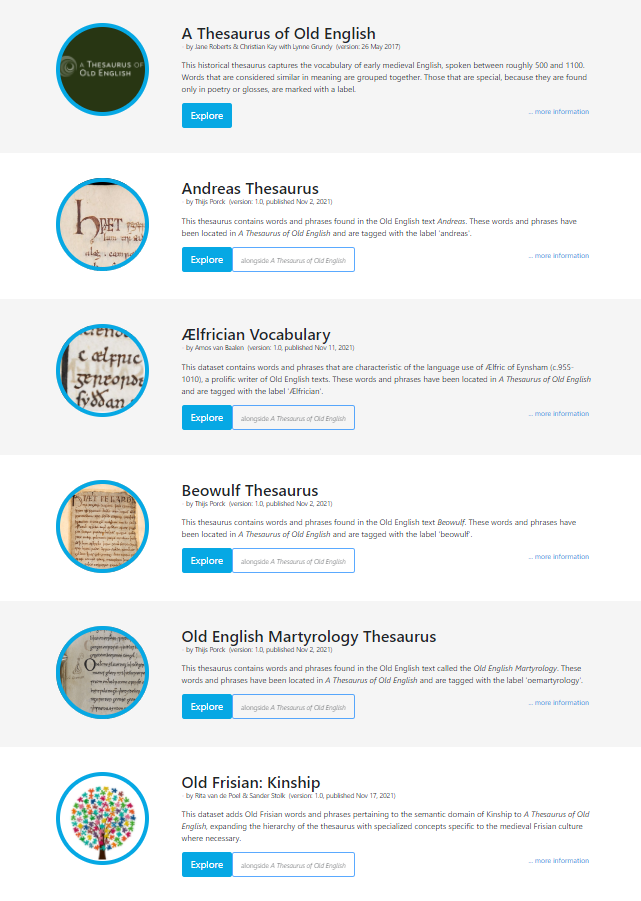
\includegraphics[width=0.75\textwidth]{Stolk2021x/fig/Evoke-content-short.png}
	\caption[]{\label{fig:Stolk2021x:Evoke-content}Overview of content available in Evoke at\\\url{http://evoke.ullet.net/content/}.}
\end{figure}

\newpage

\noindent
\textbf{Andreas Thesaurus} \\
\textit{Creator:} Thijs Porck \\
\textit{Version:} 1.0 \\
\textit{Released:} 2 November 2021 \\
\textit{License:} CC-BY-SA \\
{\textit{Availability:} 
\vspace{-\topsep}
\begin{itemize}
\setlength{\itemsep}{0pt}
\setlength{\parskip}{0pt}
\setlength{\parsep}{0pt}
\item in Evoke: \url{http://evoke.ullet.net/content/andreas/}
\item in DataverseNL: \url{https://doi.org/10.34894/IHVH0Z}
\end{itemize}}
\vspace{\baselineskip}

\noindent
\textbf{Ælfrician Vocabulary} \\
\textit{Creator:} Amos van Baalen \\
\textit{Version:} 1.0 \\
\textit{Released:} 11 November 2021 \\
\textit{License:} CC-BY-SA \\
{\textit{Availability:} 
\vspace{-\topsep}
\begin{itemize}
\setlength{\itemsep}{0pt}
\setlength{\parskip}{0pt}
\setlength{\parsep}{0pt}
\item in Evoke: \url{http://evoke.ullet.net/content/aelfric/}
\item in DataverseNL: \url{https://doi.org/10.34894/4BQ3ER}
\end{itemize}}
\vspace{\baselineskip}

\noindent
\textbf{Beowulf Thesaurus} \\
\textit{Creator:} Thijs Porck \\
\textit{Version:} 1.0 \\
\textit{Released:} 2 November 2021 \\
\textit{License:} CC-BY-SA \\
{\textit{Availability:} 
\vspace{-\topsep}
\begin{itemize}
\setlength{\itemsep}{0pt}
\setlength{\parskip}{0pt}
\setlength{\parsep}{0pt}
\item in Evoke: \url{http://evoke.ullet.net/content/beowulf/}
\item in DataverseNL: \url{https://doi.org/10.34894/TOTFGZ}
\end{itemize}}
\vspace{\baselineskip}

\noindent
\textbf{Old English Martyrology Thesaurus} \\
\textit{Creator:} Thijs Porck \\
\textit{Version:} 1.0 \\
\textit{Released:} 2 November 2021 \\
\textit{License:} CC-BY-SA \\
{\textit{Availability:} 
\vspace{-\topsep}
\begin{itemize}
\setlength{\itemsep}{0pt}
\setlength{\parskip}{0pt}
\setlength{\parsep}{0pt}
\item in Evoke: \url{http://evoke.ullet.net/content/oemartyrology/}
\item in DataverseNL: \url{https://doi.org/10.34894/QZCNW1}
\end{itemize}}
\vspace{\baselineskip}

\noindent
\textbf{Old Frisian: Kinship} \\
\textit{Creators:} Rita van de Poel and Sander Stolk \\
\textit{Version:} 1.0 \\
\textit{Released:} 17 November 2021 \\
\textit{License:} CC-BY-SA \\
{\textit{Availability:} 
\vspace{-\topsep}
\begin{itemize}
\setlength{\itemsep}{0pt}
\setlength{\parskip}{0pt}
\setlength{\parsep}{0pt}
\item in Evoke: \url{http://evoke.ullet.net/content/ofris-kinship/}
\item in DataverseNL: \url{https://doi.org/10.34894/SOLVNU}
\end{itemize}}
\vspace{\baselineskip}


\newpage
\section*{Appendix 8.B:\\Exploring Early Medieval English Eloquence workshops}
\label{Appendix8.B}

\begingroup
\renewcommand{\thefigure}{8.B.\arabic{figure}}
\setcounter{figure}{0}
\renewcommand{\thetable}{8.B.\arabic{table}}
\setcounter{table}{0}


This appendix details the three workshops within the project `Exploring Early Medieval English Eloquence' (EEMEE), initially titled `Exploring Anglo-Saxon Eloquence' (EASE). The project centred around the use of the web application Evoke and \textit{A Thesaurus of Old English} (\textit{TOE}) for use in research and education. 
%The development of Evoke has been greatly aided by the collaborative spirit of the scholars whose work is discussed in this chapter. Collegial feedback and a cooperative atmosphere helped shape everyone's efforts at the workshops in which the various case studies were developed and presented. 
Further information on the workshops and other events surrounding EEMEE and Evoke can be found at \url{http://evoke.ullet.net/events}. EEMEE was supported by the LUCAS Extra Resources Open Call-II Grant 2020, awarded by the Leiden University Centre for the Arts in Society, and the LUCDH Small Grant 2018, awarded by the Leiden University Centre for Digital Humanities.


%The functionalities listed here have been elicited in the project `Exploring Early Medieval English Eloquence', which utilizes \textit{A Thesaurus of Old English}, through dedicated stakeholder meetings, workshops, and feedback based on preliminary results in research and education.


\subsection{First workshop}

The first workshop in the series was held at Leiden University on February 1st, 2019. The full programme is shown in Figure \ref{fig:app:8.B:w1-programme}. The workshop drew attention to the web application Evoke and explored its value for various fields of research. Researchers convened to formulate potential lines of enquiry that utilise \textit{TOE} in combination with this software. The aim of the first workshop was twofold: (1) to formulate powerful and evocative case studies in research using the thesaurus, and (2) to elicit feature requests to improve the Evoke platform for research purposes. Three talks at the start of the workshop introduced participants to the two resources. 
The full programmes of the workshops are included on the last three pages of the appendix. 

After the introductory talks, the workshop continued with brainstorming on the use of the two resources in research. 
This activity was facilitated through the Change Pathway from the Europeana Impact Playbook.\footnote{See `Europeana Impact Playbook'.} This framework allowed participants to formulate lines of enquiry in terms of the intended outcomes, any resources required besides \textit{TOE} and Evoke, and the activities involved. 
Figure \ref{fig:app:8.B:w1-change} depicts the Change Pathway as filled out for Thijs Porck's proposed research concerning onomasiological profiling of the Old English text \textit{Beowulf}. During the workshop, groups of researchers reflected on each other's ideas, which were sketched in this manner, and suggested improvements. %Over the course of the EEMEE project, research ideas matured into the case studies this chapter describes. 
Subsequently, feature requests for Evoke were elicited based on these ideas. On handouts, researchers could describe functionality desired of tooling to benefit research. The results have been incorporated into the development roadmap of Evoke and can be found in Appendix \hyperref[Appendix2.A]{2.A}.

\subsection{Second workshop}

On October 17th, 2020, twelve researchers presented preliminary results of their research utilizing Evoke and \textit{TOE} in the second EEMEE workshop. Its programme is shown in Figure \ref{fig:app:8.B:w2-programme}. Old English language and culture, developments of metaphors, lexis used in specific texts or by specific authors, lexicographical practices, ways in which Old Germanic languages can be contrasted with each other, and the use of these digital resources in a classroom setting --- the great variation of these talks demonstrated the value of historical language thesauri and their potential in academic research. Discussion of the approaches and results thus far supplied participants with useful notes for refining, and advancing, their work over the next few months.

\subsection{Workshop at ICEHL-21}

A full-day workshop on working \textit{TOE} and Evoke was held at the 21st International Conference on English Historical Linguistics (ICEHL-21) on June 7th, 2021. The papers presented in this workshop demonstrated ways in which these two digital resources, at times complemented with additional data, can be used to explore exciting new aspects of Old English language and culture. Open to all ICEHL-21 attendants, the workshop discussed the results of the EEMEE case studies. The full programme is listed in Figure \ref{fig:app:8.B:w3-programme}. 

After the workshop, the majority of the case studies were developed into articles and submitted for inclusion in \textit{Amsterdamer Beiträge zur älteren Germanistik} 81.3-4. This special issue of the journal, published in November 2021, is titled `Exploring Early Medieval English Eloquence: A Digital Humanities Approach with \textit{A Thesaurus of Old English and Evoke}' and was edited by Thijs Porck and Sander Stolk.

\begin{figure}[h!]
\centering
\noindent\fbox{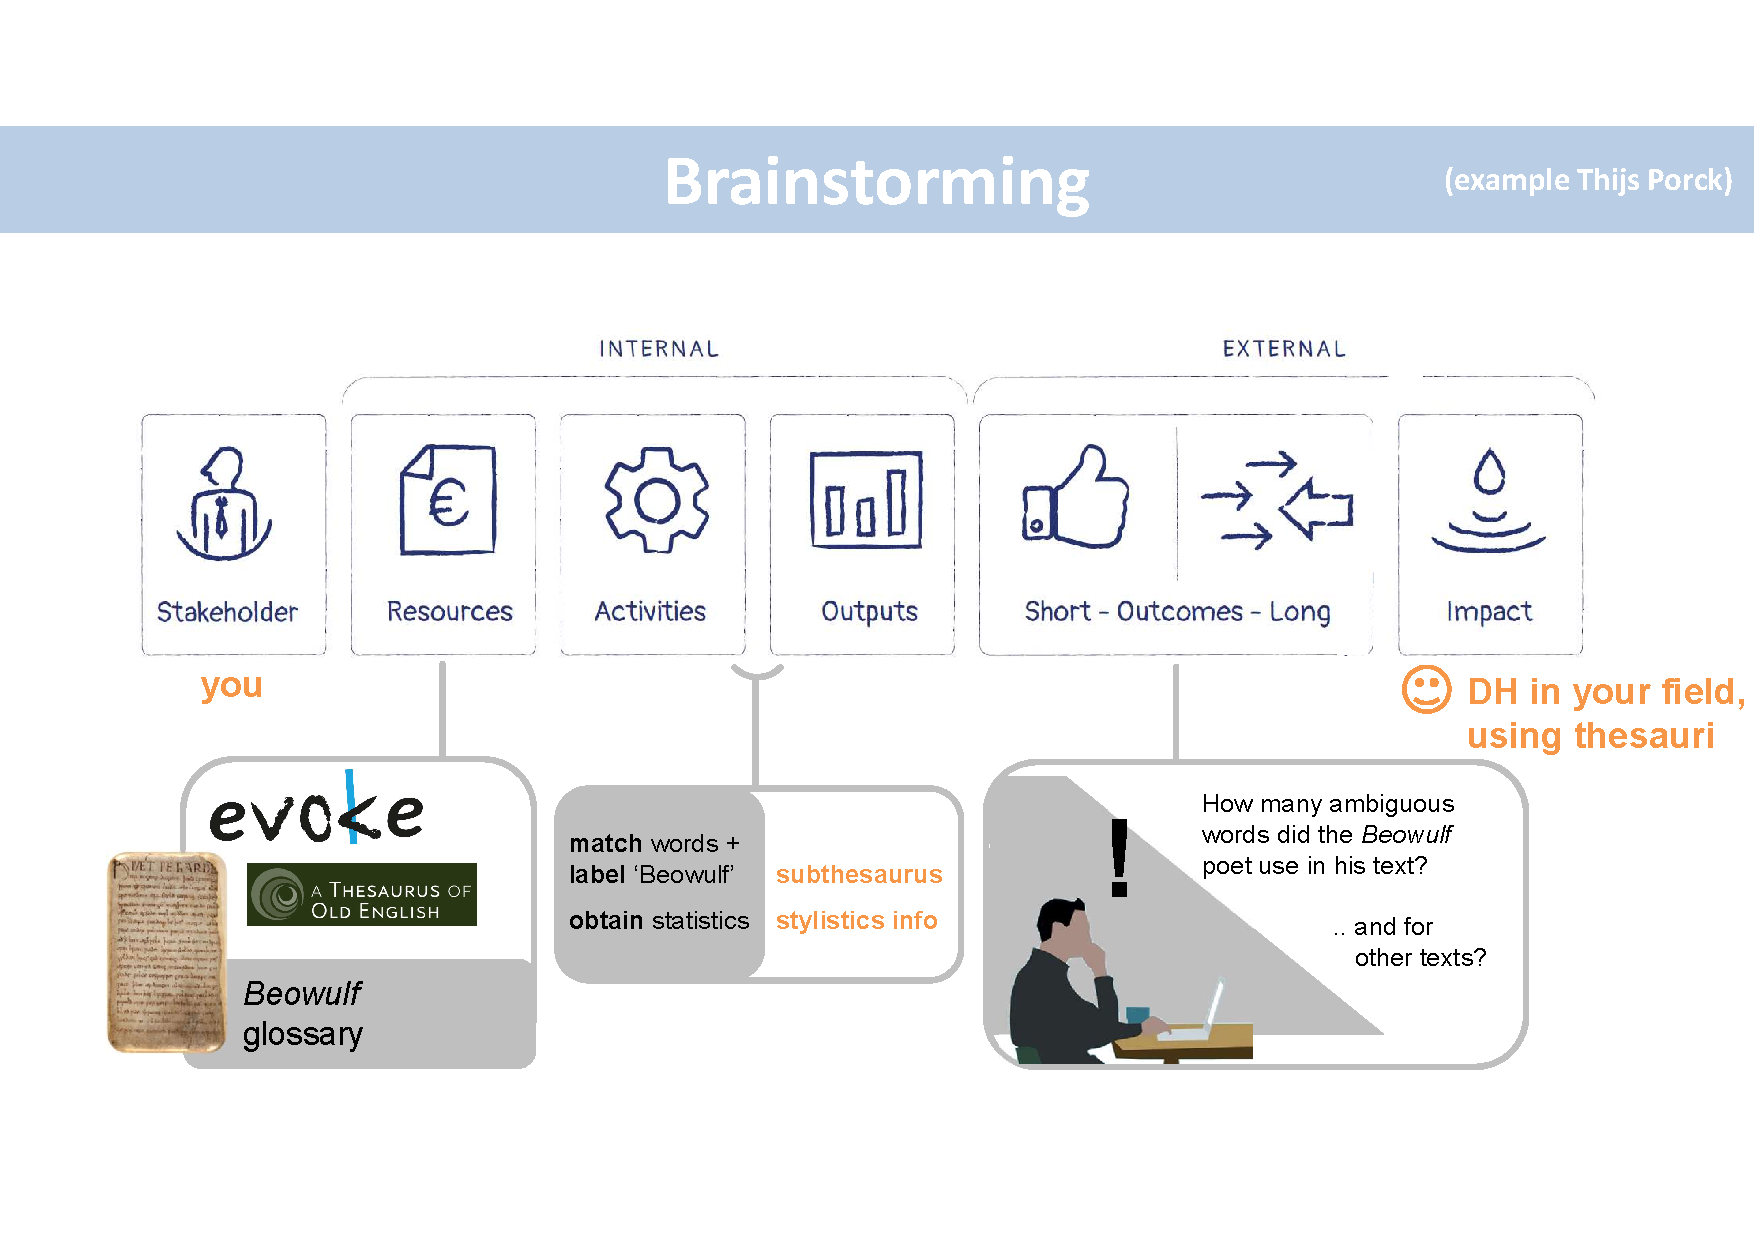
\includegraphics[width=\linewidth]{Stolk2021x/file/workshop1-changepathway.pdf}}
\caption{\label{fig:app:8.B:w1-change}Change Pathway towards onomasiological profiling of \textit{Beowulf}.}
\end{figure}


\begin{figure}[htbp!]
\centering
\fbox{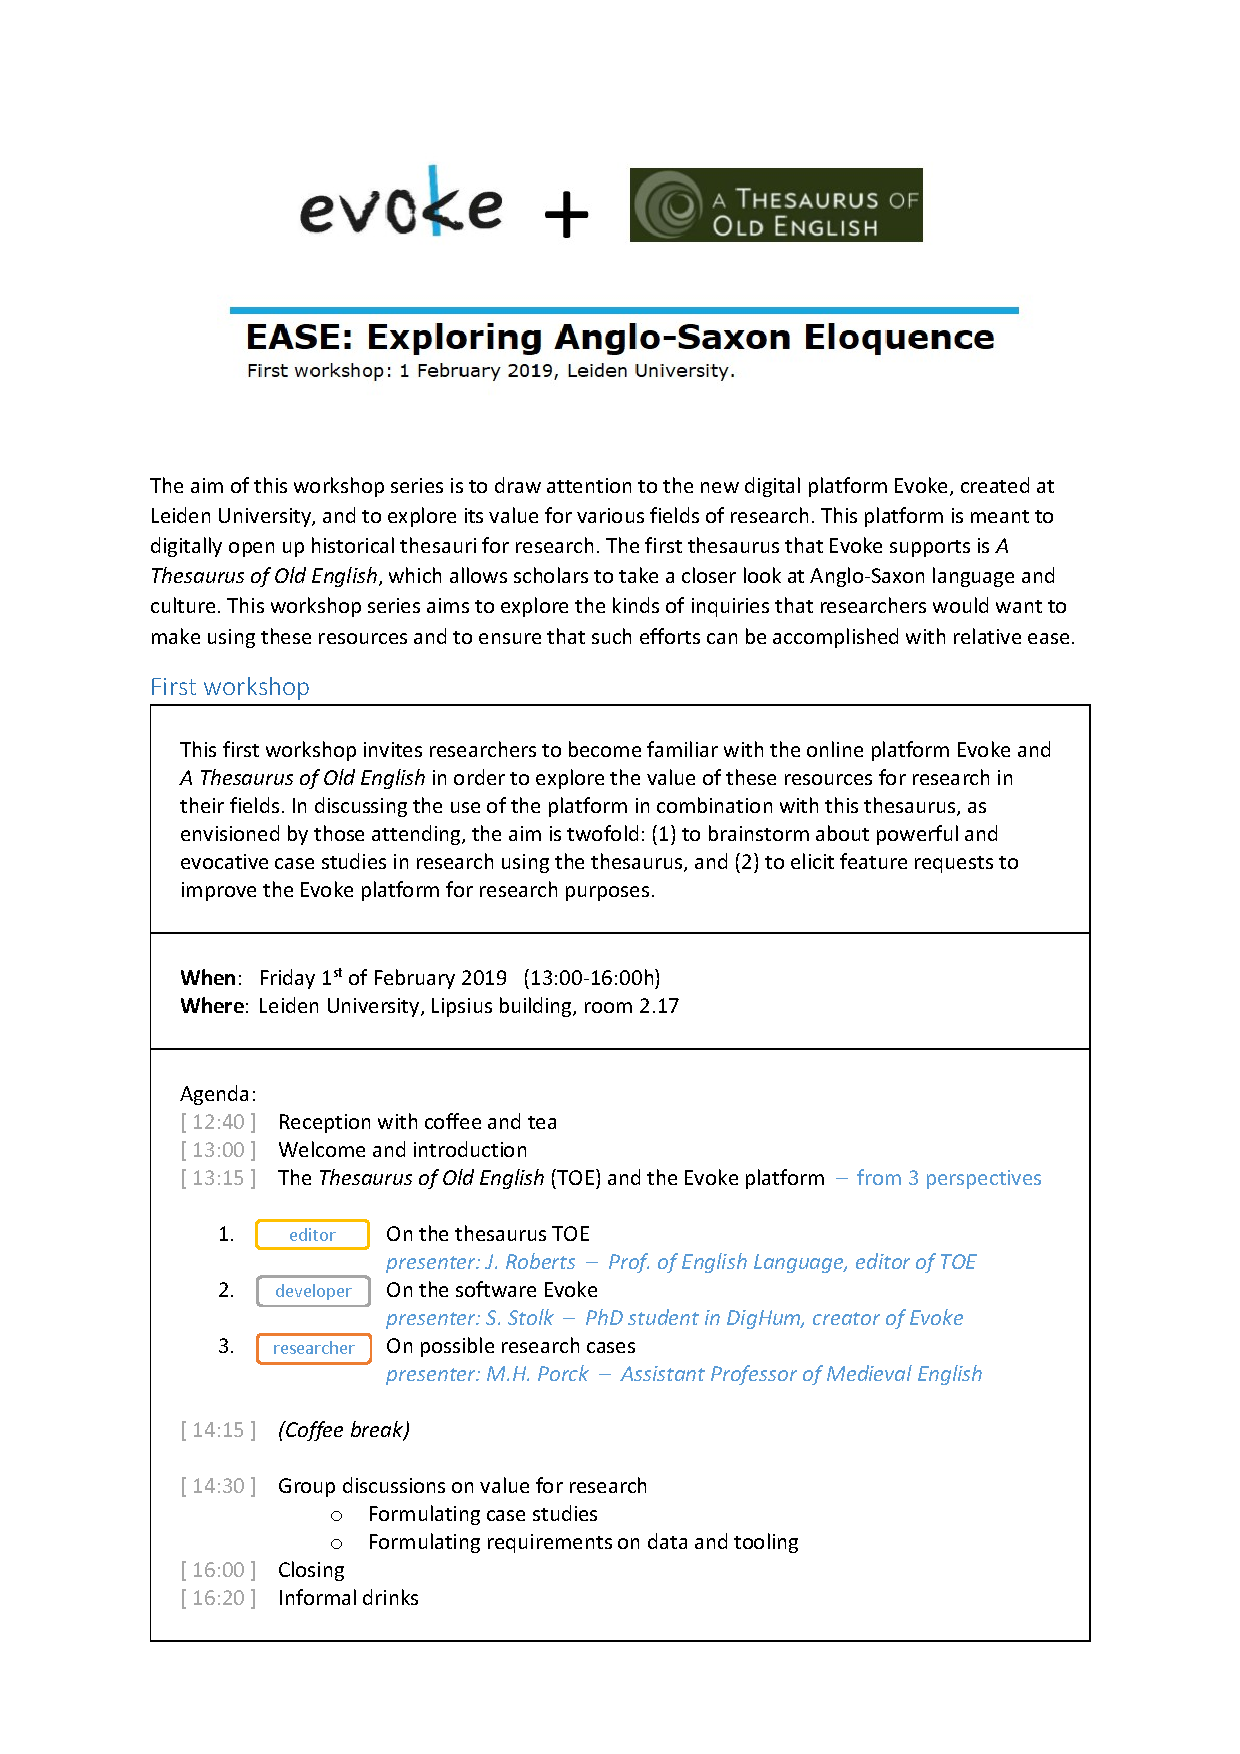
\includegraphics[width=\linewidth]{Stolk2021x/file/workshop1-programme.pdf}}
\caption{\label{fig:app:8.B:w1-programme}Programme of the first workshop.}
\end{figure}

\begin{figure}[htbp!]
\centering
\fbox{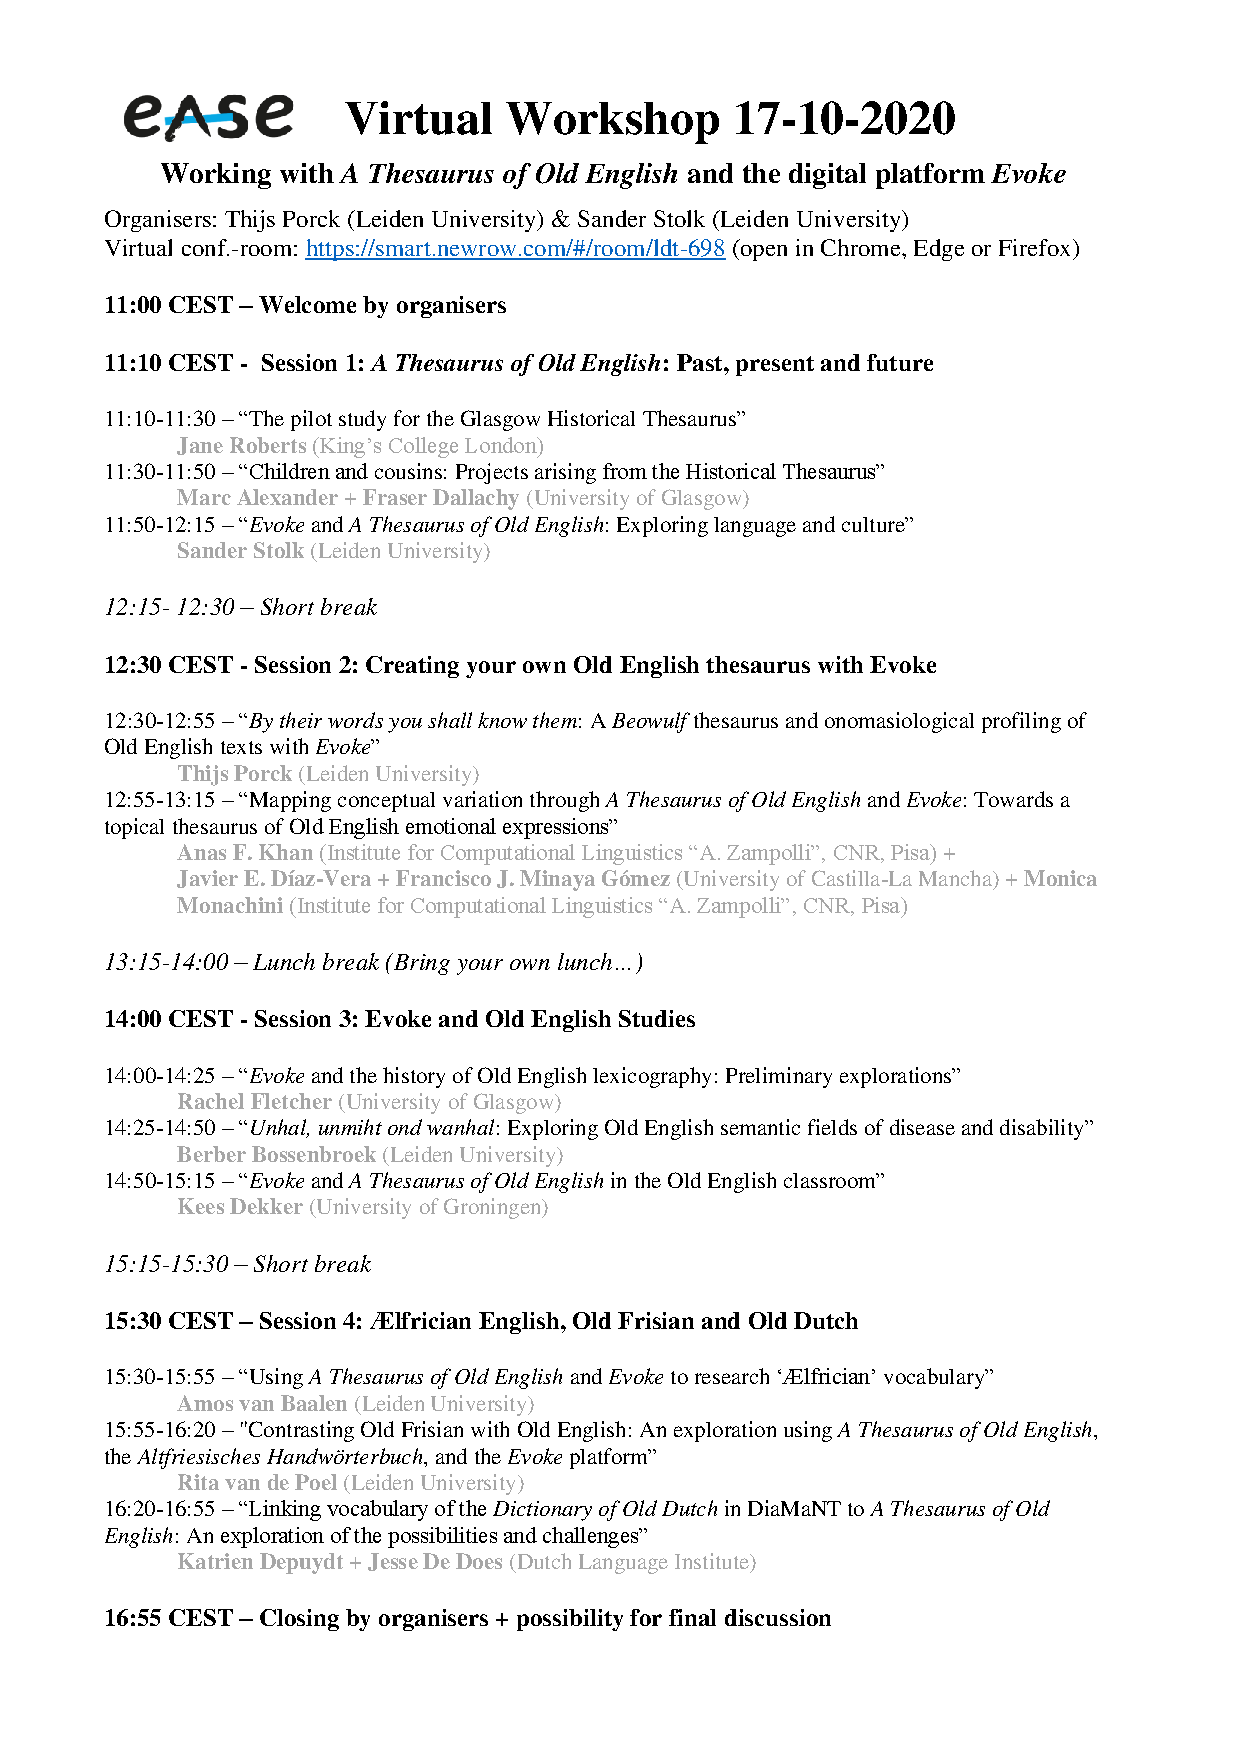
\includegraphics[width=\linewidth]{Stolk2021x/file/workshop2-programme.pdf}}
\caption{\label{fig:app:8.B:w2-programme}Programme of the second workshop.}
\end{figure}

\begin{figure}[htbp!]
\centering
\fbox{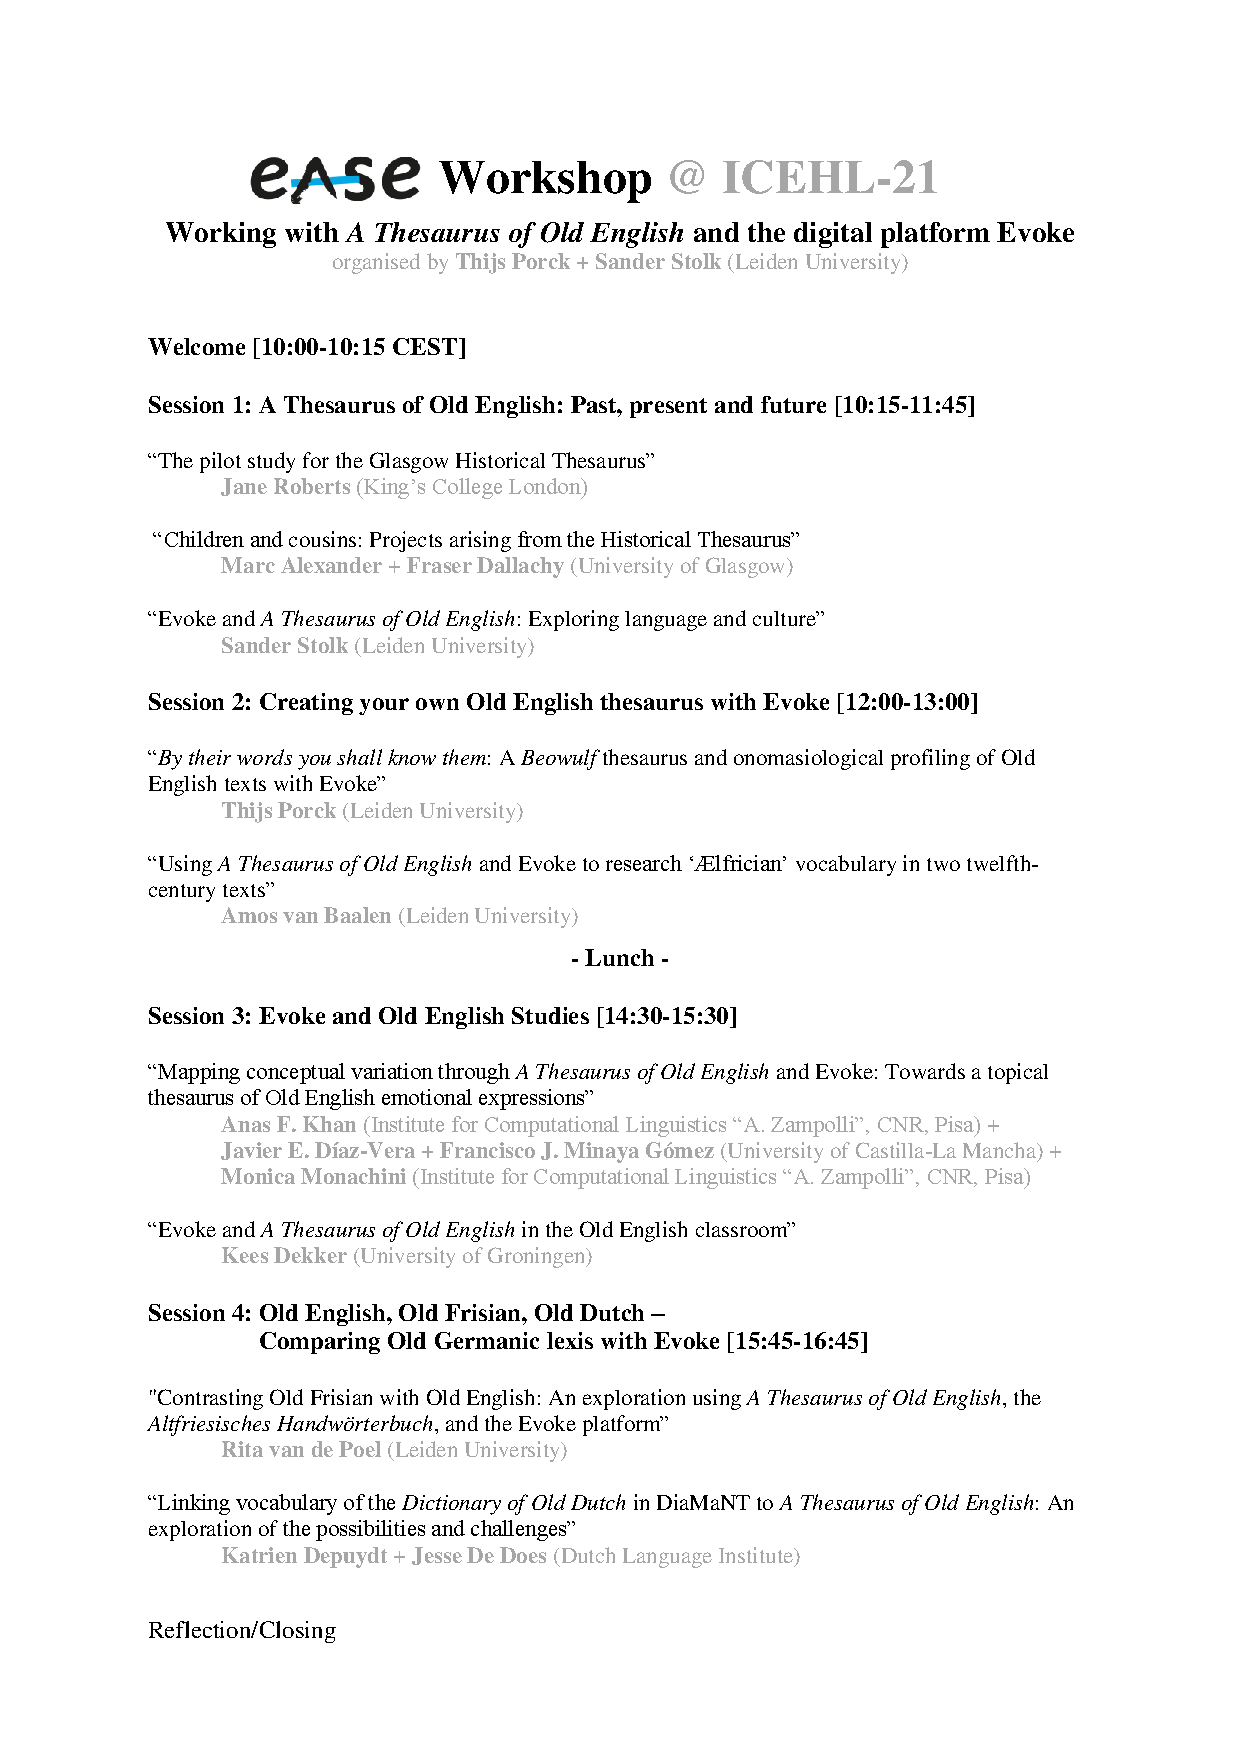
\includegraphics[width=\linewidth]{Stolk2021x/file/workshop3-programme.pdf}}
\caption{\label{fig:app:8.B:w3-programme}Programme of the third workshop.}
\end{figure}

\newpage
\section*{Appendix 8.C:\\Student-evaluation of Evoke (Nov. 2018)}
\label{Appendix8.C}

\begingroup
\renewcommand{\thefigure}{8.C.\arabic{figure}}
\setcounter{figure}{0}
\renewcommand{\thetable}{8.C.\arabic{table}}
\setcounter{table}{0}

On 13 November 2018, a small evaluation was carried out on the usefulness of Evoke in education. This evaluation took place in a 2-hour workshop, as part of a third-year Bachelor course on Old English at Leiden University, on digital resources for studying the language and culture. In the workshop, twenty-two students worked on assignments that revolved around the information available in \textit{A Thesaurus of Old English} to study Old English language and culture. The evaluation contrasted the usefulness of Evoke with that of the existent \textit{TOE} website, made available by the University of Glasgow (UoG).\footnote{The evaluation was performed on Evoke v1.2.0 and UoG's \textit{TOE4}.} The intention was to ensure that the typical classroom setting was disturbed as little as possible (and therefore to avoid the introduction of foreign elements, such as cameras and microphones) whilst still yielding valuable information on the user experience in education.

During the workshop, students were asked to form pairs; one student would work with Evoke, the other with UoG. In the workshop section devoted to \textit{TOE}, each student first got acquainted with the website assigned to them over the time span of five minutes. They were asked to explore how these websites could be navigated and what the options were that they offered, informing each other of their findings afterwards. The subsequent thirty minutes were spent on worksheets with assignments on the \textit{TOE} data. These were to be solved individually, using the assigned website, with the possibility to obtain help from the paired student when needed. After these assignments, both pieces of software were evaluated by the students.

In order to assess the usefulness of Evoke in a classroom setting, fundamental aspects were evaluated that, combined, establish a set of metrics on usefulness. Usefulness can be described as a combination of utility (i.e., the extent to which the application provides the necessary features to support users' needs) and usability (i.e., the ease with which the user interface can be used).\footnote{See, for instance, Nielsen Norman Group's methodologies for evaluating user experience. \url{https://www.nngroup.com/articles/usability-101-introduction-to-usability/}} Usability, in turn, can be broken down further into various aspects to facilitate a more fine-grained evaluation. Table \ref{table:Stolk2021x:eval:usability-aspects} lists five key aspects of usability. 
The classroom setting allowed evaluation of three of the five aspects on usability: learnability, efficiency, and satisfaction. Memorability and errors were not measured, since students would, during this workshop, be getting acquainted with the user interface of Evoke. The three evaluated aspects of usability were included alongside utility and an overall impression on usefulness.

\begin{table}[htbp]
    \centering
    \begin{tabular}{p{1in}p{3.75in}}
    \toprule
        \textbf{Aspect} & \textbf{Description} \\ 
    \midrule
        learnability & the ease with which first-time users can accomplish basic tasks \\
        efficiency & the speed with which users can perform tasks \\
        memorability & the extent to which users remember how to work with the interface after not having used it for an extended period \\
        errors & the number and severity of mistakes users make \\
        satisfaction & the pleasantness of the design and its use \\
    \midrule
    \end{tabular}
    \caption[]{\label{table:Stolk2021x:eval:usability-aspects}Key aspects of usability}
\end{table}


The evaluation of Evoke and UoG, across various aspects of usefulness, was performed through a short poll on each aspect. In order to remove bias from these polls, the evaluation drew on the Microsoft Desirability Toolkit,\footnote{Benedek and Miner, `Measuring Desirability'.} which consists of a list of 118 words or phrases for possible reactions (e.g., ``convenient'', ``difficult'', ``boring''). The students were asked to select the words that best described their stance towards the aspect under consideration, which was introduced by a short phrase (e.g., ``The look/visuals of that website'' for the aspect of satisfaction). Their possible answers, in the form of these reaction words, were narrowed down to a maximum of ten that were suitable for the aspect in question (such as ``fast'' and ``slow'' for efficiency). 

The results of the evaluation are shown in the tables below for both users of Evoke (ten out the twenty-two students) and UoG (twelve students).\footnote{The discrepancy with the number of students working with Evoke and with UoG is the result of one pair of students, out of the eleven pairs, having misunderstood their distinctive roles and worked with UoG both.} A wordcloud next to each table visualizes the results for Evoke, specifically, with scale and darkness of a word or phrase representing the relative number of users that selected it. These results show that both Evoke and UoG were received positively by the students, on both matters of utility and usability. When contrasting the two websites in the results, the most striking differences include that Evoke was more often considered to offer ``desirable'' functionality, which students later indicated was mostly owing to the statistics generated by the application, and ``fun'' to use in the assignments. 

%\subsection{Utility}
%``The functionality offered by that website''

\begin{table}[htbp]
\begin{minipage}{.7\textwidth}
    \begin{tabular}{p{1in}ccc}
    \toprule
        \textbf{Word} & \textbf{Value} & \textbf{Evoke users} & \textbf{UoG users} \\ 
    \midrule
        Desirable & + & 50 \% & 17 \% \\
        Ineffective & - & 10 \% & 17 \% \\
        Powerful & + & 20 \% & 8 \% \\
        Helpful & + & 100 \% & 100 \% \\
        Dated & - & 0 \% & 0 \% \\
        Cutting edge & + & 30 \% & 8 \% \\
        Irrelevant & - & 0 \% & 0 \% \\
        Not valuable & - & 0 \% & 0 \% \\
        Poor quality & - & 0 \% & 0 \% \\
        Useful & + & 100 \% & 92 \% \\
    \midrule
    \end{tabular}
    \caption[]{\label{table:Stolk2021x:eval:Evoke-utility}Results for Evoke on utility\\(``The functionality offered by that website'')}
\end{minipage}
\begin{minipage}{.25\textwidth}
  \includesvg[inkscapelatex=false,width=\textwidth]{Stolk2021x/fig/eval/Evoke utility.svg}
\end{minipage}
\end{table}

%\subsection{Efficiency}
%``The efficiency with which it allowed me to perform the tasks''

\begin{table}[htbp]
\begin{minipage}{.7\textwidth}
    \begin{tabular}{p{1in}ccc}
    \toprule
        \textbf{Word} & \textbf{Value} & \textbf{Evoke users} & \textbf{UoG users} \\ 
    \midrule
        Effortless & + & 40 \% & 17 \% \\
        Annoying & - & 0 \% & 25 \% \\
        Fast & + & 70 \% & 42 \% \\
        Slow & - & 10 \% & 25 \% \\
        Disruptive & - & 10 \% & 25 \% \\
        Efficient & + & 70 \% & 50 \% \\
    \midrule
    \end{tabular}
    \caption[]{\label{table:Stolk2021x:eval:Evoke-efficiency}Results for Evoke on efficiency\\(``The efficiency with which it allowed me to perform the tasks'')}
\end{minipage}
\begin{minipage}{.25\textwidth}
  \includesvg[inkscapelatex=false,width=\textwidth]{Stolk2021x/fig/eval/Evoke efficiency.svg}
\end{minipage}
\end{table}

%\subsection{Learnability}
%``The process of learning to use that site''

\begin{table}[htbp]
\begin{minipage}{.7\textwidth}
    \begin{tabular}{p{1in}ccc}
    \toprule
        \textbf{Word} & \textbf{Value} & \textbf{Evoke users} & \textbf{UoG users} \\ 
    \midrule
        Difficult & - & 0 \% & 0 \% \\
        Straightforward & + & 60 \% & 50 \% \\
        Confusing & - & 20 \% & 33 \% \\
        Too technical & - & 0 \% & 0 \% \\
        Clear & + & 80 \% & 42 \% \\
        Incomprehensible & - & 0 \% & 0 \% \\
        Accessible & + & 60 \% & 58 \% \\
        Understandable & + & 50 \% & 75 \% \\
        Easy & + & 70 \% & 33 \% \\
        Stressful & - & 0 \% & 8 \% \\
    \midrule
    \end{tabular}
    \caption[]{\label{table:Stolk2021x:eval:Evoke-learnability}Results for Evoke on learnability\\(``The process of learning to use that site'')}
\end{minipage}
%\begin{minipage}{.05\textwidth}\end{minipage}
\begin{minipage}{.29\textwidth}
  \includesvg[inkscapelatex=false,width=\textwidth]{Stolk2021x/fig/eval/Evoke learnability.svg}
\end{minipage}
\end{table}

%\subsection{Satisfaction}
%``The look/visuals of that website''

\begin{table}[htbp]
\begin{minipage}{.7\textwidth}
    \begin{tabular}{p{1in}ccc}
    \toprule
        \textbf{Word} & \textbf{Value} & \textbf{Evoke users} & \textbf{UoG users} \\ 
    \midrule
        Attractive & + & 50 \% & 25 \% \\
        Boring & - & 10 \% & 0 \% \\
        Clean & + & 90 \% & 58 \% \\
        Overwhelming & - & 0 \% & 0 \% \\
        Calm & + & 60 \% & 58 \% \\
        New & + & 20 \% & 0 \% \\
        Cutting edge & + & 0 \% & 0 \% \\
        Unattractive & - & 0 \% & 0 \% \\
        Patronizing & - & 20 \% & 0 \% \\
        Old & - & 0 \% & 8 \% \\
        Organized & + & 80 \% & 92 \% \\
        Satisfying & + & 50 \% & 25 \% \\
    \midrule
    \end{tabular}
    \caption[]{\label{table:Stolk2021x:eval:Evoke-satisfaction}Results for Evoke on satisfaction\\(``The look/visuals of that website'')}
\end{minipage}
%\begin{minipage}{.05\textwidth}\end{minipage}
\begin{minipage}{.25\textwidth}
  \includesvg[inkscapelatex=false,width=\textwidth]{Stolk2021x/fig/eval/Evoke satisfaction.svg}
\end{minipage}
\end{table}


%\subsection{Overall}
%``My feeling of that website overall...''

\begin{table}[htbp]
\begin{minipage}{.7\textwidth}
    \begin{tabular}{p{1in}ccc}
    \toprule
        \textbf{Word} & \textbf{Value} & \textbf{Evoke users} & \textbf{UoG users} \\ 
    \midrule
        Convenient & + & 70 \% & 67 \% \\
        Frustrating & - & 10 \% & 33 \% \\
        Valuable & + & 20 \% & 25 \% \\
        Useful & + & 80 \% & 100 \% \\
        Poor quality & - & 0 \% & 0 \% \\
        Essential & + & 20 \% & 8 \% \\
        High quality & + & 30 \% & 8 \% \\
        Dated & - & 0 \% & 0 \% \\
        Fun & + & 90 \% & 25 \% \\
        Professional & + & 20 \% & 50 \% \\
    \midrule
    \end{tabular}
    \caption[]{\label{table:Stolk2021x:eval:Evoke-overall}Results for Evoke on overall perception\\(``My feeling of that website overall...'')}
\end{minipage}
\begin{minipage}{.25\textwidth}
  \includesvg[inkscapelatex=false,width=\textwidth]{Stolk2021x/fig/eval/Evoke overall.svg}
\end{minipage}
\end{table}

\endgroup